\documentclass[11pt,a4paper]{report}
\usepackage[T1]{fontenc}
\usepackage{lmodern}
\usepackage[margin=2.6cm]{geometry}
\usepackage{amsmath,amssymb,bm,graphicx,booktabs,array,xcolor,url}
\usepackage[numbers,sort&compress]{natbib}
\usepackage[colorlinks=true,allcolors=blue!50!black]{hyperref}
\usepackage{microtype}
\newcolumntype{L}[1]{>{\raggedright\arraybackslash}p{#1}}
\DeclareRobustCommand{\_}{\leavevmode\kern.06em\vbox{\hrule width.3em}\penalty\exhyphenpenalty\hskip0pt\relax}
\setlength{\emergencystretch}{3em}
% Shared notation for the Dark-SPECTRAX explanatory note (writer A).
% Units: c = omega_pe = n = 1 unless stated.  Use \providecommand so repeated \input is harmless.
\providecommand{\vq}{v_q/v_{te}}
\providecommand{\wpe}{\omega_{pe}}
\providecommand{\wpi}{\omega_{pi}}
\providecommand{\wL}{\omega_L}
\providecommand{\OmD}{\Omega_D}
\providecommand{\mD}{m_D}
\providecommand{\vte}{v_{te}}
\providecommand{\lDe}{\lambda_{De}}
\providecommand{\Wext}{W_{\rm ext}}
\providecommand{\Wlin}{W_{\rm lin}}
\providecommand{\nTV}{nT_eV}
\providecommand{\Eth}{E_{\rm th}}
% vectors and fields
\providecommand{\bE}{\mathbf E}
\providecommand{\bB}{\mathbf B}
\providecommand{\bA}{\mathbf A}
\providecommand{\bJ}{\mathbf J}
\providecommand{\bv}{\mathbf v}
\providecommand{\bx}{\mathbf x}
\providecommand{\bk}{\mathbf k}
\providecommand{\bp}{\mathbf p}
\providecommand{\bu}{\mathbf u}
\providecommand{\ED}{\mathbf E_D}
\providecommand{\BD}{\mathbf B_D}
\providecommand{\AD}{\mathbf A_D}
\providecommand{\phiD}{\phi_D}
\providecommand{\Edrive}{\mathbf E_{\rm drive}}
% operators and constants
\providecommand{\dd}{\mathrm{d}}
\providecommand{\ee}{\mathrm{e}}
\providecommand{\ii}{\mathrm{i}}
\providecommand{\pd}[2]{\frac{\partial #1}{\partial #2}}
\providecommand{\Real}{\operatorname{Re}}
\providecommand{\Imag}{\operatorname{Im}}
\providecommand{\avg}[1]{\langle #1\rangle}
\providecommand{\Hn}{H_n}
\providecommand{\Ham}{\mathcal H}

\title{Dark-photon conversion in plasma:\\ an explanatory note on the Dark-SPECTRAX study}
\author{Rog\'erio Jorge}
\date{\today}
\begin{document}
\maketitle
\chapter*{Preface}
\addcontentsline{toc}{chapter}{Preface}
This note is the long companion to the paper on relativistic detuning, electron heating and the reach of continuum kinetic methods in resonant dark-photon conversion in a plasma. The paper reports results in a few pages. The note explains what the paper takes for granted: the field theory of the dark photon, the kinetic theory against which the numerical results are judged, the numerical methods, the way they are assembled in Dark-SPECTRAX, and the studies themselves with their failures.

The first four chapters set up the physics and the methods and can be read independently of the rest. Chapters 5 to 7 describe the model and its implementation, the verification ladder and the limits of the nonrelativistic Hermite solver. Chapters 8 to 10 take up the claim of Hook, Huang and Shalaby, the nonrelativistic studies and the relativistic ones, and Chapter 11 collects what is settled and what is open. Appendix A lists the repositories, pins and records so that every number can be traced. Quantities are quoted from the repository records and from the paper; where a derivation was done for the note itself, the text says so. Units are $c=\omega_{pe}=n=1$ unless stated otherwise.
\tableofcontents
\clearpage
\chapter{Introduction}\label{ch:intro}

This note accompanies the paper on relativistic detuning, electron heating and the reach of continuum kinetic methods in resonant dark-photon conversion in a plasma. The paper is a short report of results. The note is the long version of everything the paper takes for granted: the field theory of the dark photon, the kinetic plasma theory that is used to judge the numerical results, the numerical methods and the way they are put together in Dark-SPECTRAX. It is meant for a reader who knows classical electrodynamics and some kinetic theory and wants to follow the argument without going through twenty references first. The chapters are independent enough to be read in isolation; Chapters~\ref{ch:darkphoton} to~\ref{ch:numerics} are self-contained derivations, and the later chapters use them to discuss the results.

\section{Why this problem}

Dark matter has not been detected through any non-gravitational interaction, and the search has widened from weakly interacting particles of GeV mass to very light bosons, which behave as classical fields when their occupation numbers are large. One of the simplest candidates is a massive vector boson, a dark photon, that mixes kinetically with the ordinary photon. Its Lagrangian has one extra gauge field, one mass and one dimensionless mixing parameter $\chi$, and because the mixing is a renormalizable operator it can be generated by heavy particles charged under both gauge groups at loop level~\citep{Holdom1986}. The review of Fabbrichesi, Gabrielli and Lanfranchi collects the theory and the laboratory and astrophysical searches~\citep{Fabbrichesi2020}. If its mass lies below roughly an electron volt and a mechanism populates the field in the early Universe, the dark photon behaves as cold dark matter, with a coherent field oscillating at its Compton frequency~\citep{NelsonScholtz2011,Arias2012}.

A coherent dark-photon field does not interact with a vacuum, but it does with a plasma. The kinetic mixing makes the dark field exert a force on charges that is $\eta\simeq\chi$ times the force of an ordinary field of the same strength (Sec.~\ref{sec:mixing}). In a plasma the electrons oscillate collectively at the plasma frequency $\wpe$, and when $\wpe$ equals the dark-photon mass the dark field drives this oscillation resonantly, in the way a swing is driven by a push at its natural frequency. In the early Universe the free electrons and protons that survive recombination form a plasma whose density, and hence $\wpe$, falls with expansion. For a dark photon of any mass in a wide range there is a moment at which the plasma frequency sweeps through the mass. Energy then moves from the dark field into plasma oscillations, which damp and heat the gas. The effect is the plasma analogue of the conversion of dark photons into photons in a medium, and its Landau--Zener description is the subject of Sec.~\ref{sec:resonance}~\citep{Mirizzi2009,DubovskyHC2015,McDermottWitte2020}.

\section{The bounds and the claim of Hook, Huang and Shalaby}

Heating of the intergalactic gas and distortions of the cosmic microwave background by conversion at the resonance put limits on the mixing as a function of the dark-photon mass. The dark-photon limits are summarized in a recent handbook~\citep{CaputoHandbook2021}, and the cosmological ones depend on how much of the dark-matter energy is deposited in the plasma when the resonance is crossed~\citep{McDermottWitte2020,Witte2020}. The calculation assumes that the transfer is described by linear response: the dark field drives a longitudinal plasma oscillation, the oscillation is damped by collisions or by Landau damping, and the energy ends up as heat. In this picture the deposited energy is a fixed fraction of the dark-matter energy density that depends on the Landau--Zener adiabaticity parameter of Eq.~\eqref{eq:LZ}, and nothing limits the amplitude of the plasma oscillation until the resonance is passed.

Hook, Huang and Shalaby (HHS) argued that this picture fails because of plasma nonlinearity~\citep{HHS2026}. Their reasoning is that at resonance the amplitude of the $k=0$ Langmuir oscillation grows secularly, and once the energy density of the wave approaches the thermal energy of the plasma, the ponderomotive force of the wave pushes the electrons and ions into density inhomogeneities. The plasma frequency becomes a function of position, the resonance is detuned in each region, and conversion stops. They support this with one-dimensional relativistic particle-in-cell simulations, with a prescribed spatially uniform dark-photon drive, mass ratio $m_i/m_e=1836$, and drive strengths $v_q/v_{te}=0.03$ and $10^{-3}$, where $v_q=E_0/\wpe$ is the velocity scale of the drive (Sec.~\ref{sec:resonance}), and with Landau--Zener sweeps. The energy deposited is of the order of the electron thermal energy at the time of conversion, which they find to be orders of magnitude below the amount assumed in the cosmological bounds, so that the constraints weaken by factors between $3\times10^3$ and $10^7$ over ten decades in mass. The result was published as Phys.\ Rev.\ Lett.\ 137, 071004. It is a strong claim: if it holds, it removes a class of published bounds, and it rests on a numerical experiment.

The main conclusion of the claim is physical and the supporting evidence is numerical, and the numerical method has a feature that matters. A particle-in-cell simulation represents the plasma by a finite number of particles and it is noisy; the noise is not a defect to be removed, because it is also a property of the real plasma, in which there are thermal fluctuations with the same spectrum, only at a lower relative amplitude owing to the number of particles. If the instabilities that stop the transfer are seeded by noise, then the saturated state depends on the noise level, which in a PIC code is set by the number of particles per cell, and the question of which number is the physically correct one is not trivial.

\section{What a noise-free kinetic method can and cannot settle}

A continuum kinetic method represents the distribution function itself. It has no particle noise, so each run is deterministic, the work done by the drive and the energy of the fields and of the plasma are known with an energy ledger that closes to the tolerance of the integrator, and results at different resolutions can be compared without averaging over seeds. The method of this note represents the distribution in velocity by Hermite functions and in space by Fourier modes (Chapter~\ref{ch:numerics}). It can compute the linear response to the accuracy of the discretization and compare it with the exact kinetic roots, and it can run a prescribed resonant drive and measure when the response departs from the linear law. With it we can decide whether a given departure is due to a process present in the equations (as opposed to noise), by turning the process off: removing the ions, fixing the temperature, switching between nonrelativistic and relativistic kinematics, or changing the basis. Because the right-hand side is a smooth function of the model parameters, the same method can in principle be differentiated.

It also has limits, which determine what can be said about HHS. A spectral method is not positivity-preserving: the truncated expansion can give a negative distribution function once structures finer than the resolution develop. For the asymmetrically weighted basis it has in addition a numerical instability that bounds the length of a reliable run; the paper defines certified windows by declared checks and reports only what is inside them. The method cannot represent cell-scale shot noise as a physical fluctuation, because with PIC-like particle numbers its distribution function loses positivity almost immediately. Three-dimensional velocity space and magnetized plasmas are available in the code, but the production runs are one-dimensional; collisions are included only in the nonrelativistic model and with a velocity-independent frequency. The method is not a substitute for cosmological modelling: it knows nothing of expansion, cooling by Compton scattering or the temperature-dependent collision frequency.

With these capabilities the questions that the method can settle are the following. Where, in a model with the physical ingredients of HHS, does the energy transfer from a resonant uniform drive leave the linear resonant law? What sets the timing of that departure? What is the heating that HHS plot, and can a deterministic calculation produce it? The answers of the paper, which the later chapters derive and qualify, are short. The timing is that of relativistic detuning, the decrease of the plasma frequency of the quivering electrons as their mass grows: both relativistic continuum models leave the linear law by 10\,\% at $\wpe t\simeq392.5$ for $\vq=0.03$, and the homogeneous relativistic Vlasov equation at $k=0$, a few lines of code, gives 392.3 (Sec.~\ref{sec:relativistic}). The heating is a different matter. An independent relativistic PIC converges to about 25 initial thermal energies at $\wpe t=1000$, half the 50 read off the figure of HHS, a Newtonian pusher gives 63, and the deterministic continuum codes give $0.056$, a factor of 445 below the PIC. The origin of the factor of two between the PIC and HHS is not resolved, and whether finite-amplitude fluctuations absent from the continuum seeds produce the heating is an open question. We do not claim that HHS is wrong.

The nonrelativistic results that preceded the relativistic ones are retained with their scope marked. They concern a model whose coherent quiver speed reaches $0.47$--$0.87c$ at the ends of its certified windows (1000, 892 and 791.5 at $\vq=0.03$, 0.05 and 0.07), so they are statements about that model and not about a relativistic plasma (Chapter~\ref{ch:nonrel}).

\section{Roadmap}

The remainder of the first part of the note has three chapters. Chapter~\ref{ch:darkphoton} derives the dark-photon model from the kinetic-mixing Lagrangian and its coupling to a plasma, including the resonance and the Landau--Zener passage. Chapter~\ref{ch:plasma} collects the kinetic plasma theory against which the numerical results are judged, from Landau damping to the parametric instabilities of a uniform pump that are central to the HHS argument, and ends with the relativistic oscillator. Chapter~\ref{ch:numerics} describes the numerical methods, particle-in-cell, grid, discontinuous Galerkin and Hermite, and the way they appear in Dark-SPECTRAX. Chapters~\ref{ch:model} to~\ref{ch:limits} then specify the model that is solved, the ladder of verification and the limits of the Hermite solver, and Chapters~\ref{ch:hhs} to~\ref{ch:rel} take up the HHS claim and the nonrelativistic and relativistic studies. Chapter~\ref{ch:discussion} collects what is settled and what is open, and Appendix~\ref{app:repro} lists repositories, pins and records.

Units are $c=\wpe=n=1$ unless stated, with $\vq=v_q/v_{te}$ for the drive strength. Numbers quoted from the repository carry their record or section in a parenthesis or footnote, with paths relative to the repository root. Where the note computes something that is not in a record, it says so and gives the script (\texttt{note/make\_note\_figures.py}). Literature is cited where it is used, and only for statements that the cited work contains.

\chapter{The dark photon as a field coupled to a plasma}\label{ch:darkphoton}

The introduction posed the problem in words; this chapter turns it into equations. It collects what is needed from field theory and electrodynamics to write down the equations that Dark-SPECTRAX solves. It starts from the kinetic-mixing Lagrangian, removes the mixing by a field redefinition, studies the resulting massive vector field in vacuum, couples it to a plasma, and proves the energy theorem that the code uses as a check on every run. It ends with the resonance between the dark photon and the plasma oscillation, the Landau--Zener description of a resonance crossed in a density gradient, and a short account of how the cosmological bounds are built. Units are $\hbar=c=\epsilon_0=1$ in the field-theory sections; the plasma sections restore $c$ and $\epsilon_0$ where they matter.

\section{Kinetic mixing and the canonical form}\label{sec:mixing}

A dark photon is a vector field $A'_\mu$ of an extra $U(1)$ gauge group under which no Standard Model particle is charged. Two abelian field strengths $F_{\mu\nu}=\partial_\mu A_\nu-\partial_\nu A_\mu$ and $F'_{\mu\nu}$ can be contracted with each other, and the resulting operator is gauge invariant and renormalizable. Holdom noted that integrating out heavy particles charged under both groups generates it at loop level~\citep{Holdom1986}, and the idea of a second, hidden photon is older. The Lagrangian, with the metric signature $(+,-,-,-)$ and a Standard Model current $J^\mu$ coupled to the photon, is
\begin{equation}
\mathcal L=-\tfrac14F_{\mu\nu}F^{\mu\nu}-\tfrac14F'_{\mu\nu}F'^{\mu\nu}-\tfrac{\chi}{2}F_{\mu\nu}F'^{\mu\nu}+\tfrac12m_0^2A'_\mu A'^\mu-J^\mu A_\mu .
\label{eq:Lmix}
\end{equation}
The dimensionless number $\chi$ is the kinetic mixing and $m_0$ the bare mass of the dark photon, which may arise from a Higgs or a St\"uckelberg mechanism; the review of Ref.~\citep{Fabbrichesi2020} describes both. No mass term for $A_\mu$ is allowed, because the photon stays massless in vacuum.

The kinetic terms of Eq.~\eqref{eq:Lmix} are not canonical, since the quadratic form $F^2+F'^2+2\chi FF'$ has off-diagonal entries. We remove them by a linear change of variables that is not an orthogonal rotation. Write
\begin{equation}
A_\mu=\tilde A_\mu+\frac{\chi}{s}\tilde A'_\mu,\qquad A'_\mu=-\frac{1}{s}\tilde A'_\mu,\qquad s\equiv\sqrt{1-\chi^2}.
\end{equation}
Then $F=\tilde F+(\chi/s)\tilde F'$ and $F'=-\tilde F'/s$, and the three quadratic terms combine as
\begin{align}
F^2+F'^2+2\chi FF'&=\tilde F^2+\frac{2\chi}{s}\tilde F\tilde F'+\frac{\chi^2}{s^2}\tilde F'^2+\frac{1}{s^2}\tilde F'^2-\frac{2\chi}{s}\tilde F\tilde F'-\frac{2\chi^2}{s^2}\tilde F'^2\nonumber\\
&=\tilde F^2+\frac{1+\chi^2-2\chi^2}{s^2}\tilde F'^2=\tilde F^2+\tilde F'^2 ,
\end{align}
so the cross term has cancelled and both fields are canonical. The mass term becomes $\tfrac12(m_0^2/s^2)\tilde A'_\mu\tilde A'^\mu$, so the physical mass of the dark photon is
\begin{equation}
m_D=\frac{m_0}{\sqrt{1-\chi^2}} ,\label{eq:mD}
\end{equation}
and the current couples as $-J^\mu A_\mu=-J^\mu(\tilde A_\mu+\eta\tilde A'_\mu)$ with
\begin{equation}
\eta=\frac{\chi}{\sqrt{1-\chi^2}} .\label{eq:eta}
\end{equation}
Dropping the tildes, the theory is that of an ordinary massless photon with its usual coupling, plus a massive vector field $A'_\mu$ that couples to every charge with $\eta$ times the electromagnetic strength. This is the form used in the Dark-SPECTRAX model~\citep{DarkSPECTRAX} and in the review of Fabbrichesi, Gabrielli and Lanfranchi, whose Sec.~1.1 gives the coupling $e\varepsilon/\sqrt{1-\varepsilon^2}$ for $\varepsilon=\chi$~\citep{Fabbrichesi2020}. We checked Eqs.~\eqref{eq:mD} and~\eqref{eq:eta} against that reference; the sign of $\eta$ depends on the sign convention for $A'_\mu$, and the model is symmetric under $\eta\to-\eta$, $\AD\to-\AD$. The case in which the dark field has no mass and the coupling is a fractional charge is a different model (``millicharged'') and is not used here. For $\chi\ll1$, which covers every cosmologically interesting case, $\eta\simeq\chi$ and $m_D\simeq m_0$ to relative corrections of order $\chi^2$.

A different basis is common in the cosmology literature~\citep{Mirizzi2009,Redondo2009,Arias2012}. There one keeps $A'$ as the field that does not couple to $J$ (the sterile state) and moves the mixing into the mass matrix, which then has an off-diagonal element $\chi m_0^2$ at leading order in $\chi$. The two descriptions are related by the shear above together with the identification of the photon propagating state in a medium. In the basis used here the mass matrix is already diagonal in vacuum, and the medium enters through the plasma current that couples the two fields, as it does in the simulations. Conversion happens where the effective mass of the photon-like excitation in the medium, which is the plasma frequency $\wpe$ for longitudinal oscillations, crosses $m_D$.

\section{The massive vector field}\label{sec:proca}

For the dark photon alone, with $j^\mu$ standing for whatever current is coupled to it, the Lagrangian $-\tfrac14F'^2+\tfrac12m_D^2A'^2-j\cdot A'$ gives, by varying $A'_\nu$, the Proca equation
\begin{equation}
\partial_\mu F'^{\mu\nu}+m_D^2A'^\nu=j^\nu .\label{eq:proca}
\end{equation}
We write $A'^\mu=(\phi_D,\AD)$, $\ED=-\nabla\phi_D-\partial_t\AD$ and $\BD=\nabla\times\AD$, so that $F'^{i0}=E_D^i$ and $F'^{ij}=-\epsilon^{ijk}B_D^k$. The $\nu=0$ component of Eq.~\eqref{eq:proca} reads $\partial_iF'^{i0}+m_D^2\phi_D=j^0$, that is
\begin{equation}
\nabla\!\cdot\!\ED+\OmD^2\phi_D=\rho_j ,\label{eq:gaussD}
\end{equation}
and the spatial components $\partial_0F'^{0i}+\partial_jF'^{ji}+m_D^2A'^i=j^i$ become
\begin{equation}
\partial_t\ED=\nabla\times\BD+\OmD^2\AD-\bJ_j ,\qquad \partial_t\BD=-\nabla\times\ED ,\label{eq:ampD}
\end{equation}
where the second equation is the Bianchi identity and $\OmD\equiv m_D$ is the dark-photon mass written as a frequency, the notation of the rest of the note. Compared with Maxwell's equations there are two changes. Gauss's law acquires a term $\OmD^2\phi_D$, and Amp\`ere's law acquires a term $\OmD^2\AD$. Both break gauge invariance, so the potentials are physical fields.

Taking the four-divergence of Eq.~\eqref{eq:proca} makes the first term vanish identically, because $F'^{\mu\nu}$ is antisymmetric, and leaves $m_D^2\partial_\nu A'^\nu=\partial_\nu j^\nu$. For a conserved source this is the Lorenz condition,
\begin{equation}
\partial_t\phi_D+\nabla\!\cdot\!\AD=0 ,\label{eq:lorenz}
\end{equation}
which in the Maxwell case is a gauge choice and here is a consequence of the equations. It is the evolution equation for $\phi_D$ that the code integrates (in units with $c$ restored it reads $\partial_t\phi_D=-c^2\nabla\!\cdot\!\AD$), so $\phi_D$ is a dynamical variable and Eq.~\eqref{eq:gaussD} is a constraint that is preserved by the flow. To check this, take the time derivative of $\nabla\!\cdot\!\ED+\OmD^2\phi_D$ with Eqs.~\eqref{eq:ampD} and~\eqref{eq:lorenz}: the curl term drops out, $\OmD^2\nabla\!\cdot\!\AD$ cancels against $\OmD^2\partial_t\phi_D$, and what remains is $-\nabla\!\cdot\!\bJ_j=\partial_t\rho_j$ by charge conservation.

Substituting $\ED$ and $\BD$ in terms of the potentials and using the Lorenz condition gives a Klein--Gordon equation for each component, $(\partial_t^2-\nabla^2+\OmD^2)A'^\nu=j^\nu$. In vacuum a plane wave $\ee^{\ii(\bk\cdot\bx-\omega t)}$ has the dispersion relation
\begin{equation}
\omega^2=k^2c^2+\OmD^2 .\label{eq:dispD}
\end{equation}
The four components of $A'^\mu$ are restricted by the Lorenz condition $k_\mu\varepsilon^\mu=0$ to three independent polarization vectors, in contrast to the two of a massless photon. Two are transverse, with $\phi_D=0$ and $\AD\perp\bk$; they carry $\ED=\ii\omega\AD$ and $\BD=\ii\bk\times\AD\neq0$. The third is longitudinal. In the rest frame of the mode it is $\varepsilon^\mu=(0,\hat{\mathbf n})$ for any direction $\hat{\mathbf n}$, and boosted to momentum $\bk$ it becomes $\varepsilon_L^\mu=(k,\omega\hat{\bk})/\OmD$, with $k=|\bk|$. It is normalized, $\varepsilon_L\cdot\varepsilon_L=(k^2-\omega^2)/\OmD^2=-1$, and satisfies the Lorenz condition because $\omega k-\omega k=0$. For this mode $\phi_D=ka/\OmD$ and $\AD=\omega a\hat{\bk}/\OmD$ with $a$ the amplitude, so $\phi_D$ is nonzero and equal to $(k/\omega)A_{D}$; there is no magnetic field, but there is an electric field,
\begin{equation}
\ED=\ii\omega\AD-\ii\bk\phi_D=\ii\,\frac{\omega^2-k^2}{\omega}\,\AD=\ii\,\frac{\OmD^2}{\omega}\,\AD .\label{eq:ELong}
\end{equation}
This longitudinal electric field is what couples the dark photon to charge-density oscillations of a plasma. Its coupling to a conserved current is easy to evaluate: $j_\mu\varepsilon_L^\mu=(k\rho_j-\omega\hat{\bk}\cdot\bJ_j)/\OmD$, and with $\omega\rho_j=\bk\cdot\bJ_j$ this equals $-\OmD\rho_j/k$. The amplitude to excite the longitudinal mode from a charge density is therefore proportional to $\OmD$ and vanishes in the massless limit, where $\varepsilon_L^\mu\to k^\mu/\OmD$ is a pure gauge, as it should.

The dark-photon dark matter of cosmology is the $k\to0$ limit, where the three polarizations are degenerate with $\omega=\OmD$. A coherent homogeneous field then has $\phi_D=0$, $\AD=\mathbf a\cos(\OmD t)$ and $\ED=\OmD\mathbf a\sin(\OmD t)$. The vector $\mathbf a$ sets the polarization; its orientation is random in the Universe, which is the reason why a homogeneous drive in one dimension is a legitimate idealization of the longitudinal-resonance problem. The energy density $\tfrac12(E_D^2+\OmD^2A_D^2)=\tfrac12\OmD^2a^2$ is constant. Identifying it with the dark-matter density at the redshift of interest gives the electric field amplitude that the plasma sees,
\begin{equation}
E_{D,0}=\OmD a=\sqrt{2\rho_{\rm DM}} ,\qquad E_0=\eta E_{D,0},\label{eq:E0}
\end{equation}
in Heaviside--Lorentz units, where the second equation is the amplitude of the force field $\eta\ED$ acting on a charge. The prescribed-drive mode of Dark-SPECTRAX uses $E_0\cos(\omega t+\varphi)$ for $\eta\ED$ and adds no reservoir; the self-consistent mode evolves $\ED$ itself and lets the reservoir deplete.

\section{Coupling to a plasma}\label{sec:coupling}

A particle of charge $q$ and mass $m$ in the full theory sees both fields. In the canonical form of Sec.~\ref{sec:mixing} the Lorentz force is $q[\bE+\eta\ED+\bv\times(\bB+\eta\BD)]$, and the current of all species $\bJ=\sum_sq_s\int\bv f_s\,\dd^3v$ is the source of the ordinary field with unit strength and of the dark field with strength $\eta$. Collecting the pieces, the plasma obeys the Vlasov equation
\begin{equation}
\pd{f_s}{t}+\bv\cdot\nabla f_s+\frac{q_s}{m_s}\Big[\bE+\eta\ED+\Edrive+\bv\times(\bB+\eta\BD)\Big]\cdot\pd{f_s}{\bv}=0 ,\label{eq:vlasovD}
\end{equation}
where $\Edrive$ is the optional prescribed uniform drive. The ordinary fields obey $\partial_t\bE=c^2\nabla\times\bB-\bJ/\epsilon_0$, $\partial_t\bB=-\nabla\times\bE$, with $\nabla\!\cdot\!\bE=\rho/\epsilon_0$. The dark fields obey Eqs.~\eqref{eq:gaussD}--\eqref{eq:lorenz} with the source $\eta(\rho,\bJ)$,
\begin{align}
\partial_t\ED&=c^2\nabla\times\BD+\OmD^2\AD-\eta\bJ/\epsilon_0, & \partial_t\BD&=-\nabla\times\ED,\label{eq:darkMaxwell}\\
\partial_t\AD&=-\ED-\nabla\phiD, & \partial_t\phiD&=-c^2\nabla\!\cdot\!\AD, \label{eq:darkPotentials}
\end{align}
and the constraint $\nabla\!\cdot\!\ED+\OmD^2\phiD/c^2=\eta\rho/\epsilon_0$. These are Eqs.~(1)--(3) of the paper. The plasma enters through the same current in both laws. The difference between the two fields is that in a conducting medium an ordinary electric field is reduced by the currents it drives, while the dark field has its own restoring term $\OmD^2\AD$, so a homogeneous dark field oscillating at $\OmD$ is not removed by the medium and acts on the charges as a drive of strength $\eta\ED$.

The simplest consequence is obtained for a homogeneous cold plasma, where all fields are uniform ($k=0$) and the electrons respond with $\dot{\bJ}=\wpe^2\epsilon_0(\bE+\eta\ED)$. We neglect the ions, whose response adds the small correction $\wL^2=\wpe^2(1+m_e/m_i)$ in what follows. With time dependence $\ee^{-\ii\omega t}$ the equations $\dot\bE=-\bJ/\epsilon_0$, $\dot\bJ=\epsilon_0\wpe^2(\bE+\eta\ED)$, $\dot\ED=\OmD^2\AD-\eta\bJ/\epsilon_0$ and $\dot\AD=-\ED$ give $\bJ=\ii\omega\epsilon_0\bE$, so
\begin{equation}
(\omega^2-\wpe^2)\bE=\wpe^2\eta\ED ,\qquad (\omega^2-\OmD^2)\ED=\eta\omega^2\bE ,
\end{equation}
where the second follows from $-\ii\omega\ED=\OmD^2\AD-\ii\omega\eta\bE$ and $\AD=-\ii\ED/\omega$. Eliminating the fields, the homogeneous roots satisfy
\begin{equation}
(\omega^2-\wpe^2)(\omega^2-\OmD^2)=\eta^2\wpe^2\omega^2 .\label{eq:hom}
\end{equation}
This is the avoided crossing of two oscillators. When $\wpe=\OmD$ set $x=\omega^2-\OmD^2$; then $x^2=\eta^2\OmD^2(\OmD^2+x)$ and for small $\eta$ the roots are $\omega_\pm\simeq\OmD(1\pm\eta/2)$. The two normal modes are equal superpositions of a plasma oscillation and a dark-photon oscillation, split by $\Delta\omega=\eta\OmD$. A dark field that begins as a pure dark oscillation therefore returns to its initial state, after having given its energy to the plasma, with the beat period $2\pi/(\eta\OmD)$. The repository reproduces this with a finite reservoir (the energy partition and the beat are in the conversion figure of the README and in the reservoir runs of the paper), and it is the reason why the prescribed drive, which has no reservoir, is meaningful only for times short compared with this period.

Finite wave number changes little for the transverse waves in a cold plasma, and it is worth seeing why. For $\bE,\ED\perp\bk$ and a cold electron response $\bJ=\ii(\epsilon_0\wpe^2/\omega)(\bE+\eta\ED)$, the wave equation of the ordinary field, $(k^2c^2-\omega^2)\bE=\ii\omega\bJ/\epsilon_0$, gives $(\omega^2-k^2c^2-\wpe^2)\bE=\eta\wpe^2\ED$. The transverse dark field obeys the Proca wave equation with source $\eta\bJ$, so $(\omega^2-k^2c^2-\OmD^2)\ED=\eta\wpe^2(\bE+\eta\ED)$. With $X=\omega^2-k^2c^2$ the determinant of the two equations is
\begin{equation}
X^2-\big[\wpe^2(1+\eta^2)+\OmD^2\big]X+\wpe^2\OmD^2=0 ,\label{eq:transverse}
\end{equation}
a quadratic in $X$ alone. The transverse branches are those of Eq.~\eqref{eq:hom} with $\omega^2$ replaced by $\omega^2-k^2c^2$: at every $k$ the pair of waves has the dispersion $\omega^2=k^2c^2+M_\pm^2$, where the effective masses $M_\pm^2$ are the two roots of Eq.~\eqref{eq:transverse}, which at $\wpe=\OmD$ are $M_\pm\simeq\OmD(1\pm\eta/2)$. The transverse problem is therefore a Lorentz-invariant avoided crossing, and the Landau--Zener formula of Sec.~\ref{sec:resonance} applies to the transverse conversion in a density gradient with the sweep rate evaluated at fixed $k$. The repository reproduces the finite-$k$ cold branches (test A04) to $2\times10^{-5}$ and $10^{-4}$ for the longitudinal and transverse cases.

For the longitudinal waves in a warm plasma the same elimination can be done in general. For $\bE=E\hat{\bk}$, $\bJ=\ii\omega\epsilon_0E$ from Amp\`ere's law, and in the dark sector the equations $-\ii\omega\ED=\OmD^2\AD-\eta\bJ/\epsilon_0$, $-\ii\omega\AD=-\ED-\ii k\phiD$, $-\ii\omega\phiD=-\ii kc^2\AD$ imply $\phiD=kc^2\AD/\omega$ and $\AD=-\ii\omega\ED/Q$ with $Q=\omega^2-k^2c^2$, so that
\begin{equation}
\ED=\frac{\eta Q}{Q-\OmD^2}\,E .
\end{equation}
This is the longitudinal dark field required by the plasma charge density, enhanced by $Q/(Q-\OmD^2)$ near the dark-photon pole. The kinetic response of the plasma to the total force field is $\bJ=-\ii\omega\epsilon_0\chi_e(E+\eta E_D)$, with $\chi_e$ the susceptibility of Chapter~\ref{ch:plasma}, and equating the two expressions for $\bJ$ gives $(1+\chi_e)E+\eta\chi_eE_D=0$, that is
\begin{equation}
D_L(k,\omega)\equiv(Q-\OmD^2)(1+\chi_e)+\eta^2Q\chi_e=0 .\label{eq:DL}
\end{equation}
It is the ordinary dispersion relation $\epsilon=1+\chi_e=0$ with an extra term proportional to $\eta^2$ and a pole at the dark-photon dispersion curve $Q=\OmD^2$, and the roots of $D_L$ are what the linear benchmark B00 compares with the Hermite solver. To first order in $\eta^2$ the root of $\epsilon=0$ is displaced by $\delta\omega=-\eta^2\chi_eQ/[(Q-\OmD^2)\,\partial_\omega\epsilon]$. For a Langmuir wave, $\chi_e\simeq-\wpe^2/\omega^2$ and $\partial_\omega\epsilon\simeq2\wpe^2/\omega^3$, so
\begin{equation}
\frac{\delta\omega}{\omega}\simeq\frac{\eta^2}{2}\,\frac{Q}{Q-\OmD^2} ,
\end{equation}
real and positive when $\omega^2-k^2c^2>\OmD^2$, and of order $\eta^2$ away from the pole. The corresponding shift of the damping rate comes from the imaginary part of $\chi_e$ in the same formula. The repository measures shifts of $+2.7\%$ in frequency and $-9.3\%$ in the damping rate at $\eta=0.3$ in the Landau-damping benchmark, and $-23.6\%$ in the damping at $k\lDe=0.3$ (README and docs/status.md); the sign pattern, a larger frequency and a smaller damping, is that of the formula above.

The tests that fix the sign and normalization of the coupling are the cold branches of Eq.~\eqref{eq:hom}, which Dark-SPECTRAX reproduces to $10^{-11}$ (test A03 of the status ladder), and the static Yukawa solution of $\phiD$ around a point charge, $\phi_{D,k}=\eta\rho_k/[k^2+\OmD^2]$ (A05), which follows from Eq.~\eqref{eq:gaussD} with $\ED=-\ii\bk\phiD$ and $\partial_t=0$.

\section{Energy and Poynting-like flux}\label{sec:energy}

The dark sector has a local conservation law whose form is not obvious from the Maxwell analogy, and getting it wrong gives a budget that silently fails to close. Set $c=\epsilon_0=1$. Define the energy density of the dark field
\begin{equation}
u_D=\tfrac12\big[E_D^2+B_D^2+\OmD^2(A_D^2+\phi_D^2)\big] .\label{eq:uD}
\end{equation}
Its time derivative is $\ED\cdot\partial_t\ED+\BD\cdot\partial_t\BD+\OmD^2(\AD\cdot\partial_t\AD+\phiD\partial_t\phiD)$. Insert Eqs.~\eqref{eq:darkMaxwell}--\eqref{eq:darkPotentials}. The curl terms combine through the vector identity $\ED\cdot\nabla\times\BD-\BD\cdot\nabla\times\ED=-\nabla\!\cdot\!(\ED\times\BD)$. The $\OmD^2$ terms give $\OmD^2\ED\cdot\AD+\OmD^2\AD\cdot(-\ED-\nabla\phiD)-\OmD^2\phiD\nabla\!\cdot\!\AD$; the $\ED\cdot\AD$ pieces cancel, leaving $-\OmD^2(\AD\cdot\nabla\phiD+\phiD\nabla\!\cdot\!\AD)=-\OmD^2\nabla\!\cdot\!(\phiD\AD)$. The source term is $-\eta\bJ\cdot\ED$. Collecting,
\begin{equation}
\pd{u_D}{t}+\nabla\!\cdot\!\mathbf S_D=-\eta\,\bJ\cdot\ED ,\qquad \mathbf S_D=\ED\times\BD+\OmD^2\phiD\AD .\label{eq:poyntingD}
\end{equation}
With $c$ and $\epsilon_0$ restored, the flux is $\epsilon_0c^2\ED\times\BD+\epsilon_0\OmD^2\phiD\AD$ and the energy density has $\phiD^2/c^2$ in place of $\phiD^2$. The first term is the Poynting vector. The second is new, and is the reason why we derive the theorem rather than quote it. It arises because the massive field carries momentum in its scalar potential: for the longitudinal mode, $\phiD\AD$ is the product of the two nonzero potentials and is not zero on average. Omitting $\phiD\AD$ from the flux, which is the natural thing to do if one thinks of the dark field as a copy of the electromagnetic field, breaks the flux budget; the Dark-SPECTRAX energy diagnostics include it and the test A02 (Proca vacuum) and A03 verify the closure.

The ordinary field satisfies the same law with $\OmD=0$ and the source $-\bJ\cdot\bE$. For a closed or periodic domain the fluxes integrate to zero, and adding the kinetic energy $K=\sum_s\int\tfrac12m_sv^2f_s$, whose rate is $\dot K=\int\bJ\cdot(\bE+\eta\ED)\dd^3x$ from Eq.~\eqref{eq:vlasovD}, we obtain
\begin{equation}
\frac{\dd}{\dd t}\big(K+U_\gamma+U_D\big)=\int\Edrive\cdot\bJ\,\dd^3x ,\label{eq:theorem}
\end{equation}
where $U_\gamma=\int\tfrac12(E^2+B^2)$ and $U_D=\int u_D$. The right-hand side is the external work $\Wext$ done by the prescribed drive and vanishes in the ordinary and self-consistent modes. Dark-SPECTRAX integrates the three works $W_\gamma=\int\!\!\int\bJ\cdot\bE$, $W_D=\eta\int\!\!\int\bJ\cdot\ED$ and $\Wext$ as extra variables of the ODE, with the same Runge--Kutta stages as the fields, so that $K-K_0=W_\gamma+W_D+\Wext$, $U_\gamma-U_{\gamma0}=-W_\gamma$ and $U_D-U_{D0}=-W_D$ hold to solver tolerance. The parent normalization needs one precaution: the theorem holds only if $m_s\Omega_{cs}=\Omega_0$ for every species in the units of the parent solver, which the model enforces by defining the masses from the cyclotron frequencies (Sec.~\ref{sec:architecture}). The three identities are the internal ledger checks reported in the paper; they are statements about the code, and a run that fails them is rejected before any physics is read from it.

\section{Resonant conversion and Landau--Zener passage}\label{sec:resonance}

The physical question of the paper is what happens when the dark photon oscillates at the plasma frequency. For a homogeneous plasma driven at $\omega=\wL$ by a uniform $E_0\cos\omega t$, the mean field and the current obey the driven oscillator $\dot{\bar E}=-\bar J$, $\dot{\bar J}=\wL^2(\bar E+E_0\cos\omega t)$ (units $\epsilon_0=1$), the \emph{linear resonant law}. Eliminating $\bar J$ gives $\ddot{\bar E}+\wL^2\bar E=-\wL^2E_0\cos\omega t$, and at $\omega=\wL$ the solution that starts from rest is
\begin{equation}
\bar E=-\tfrac12\,\wL E_0\,t\,\sin\wL t ,\qquad \bar J=\tfrac12E_0\wL\,(\sin\wL t+\wL t\cos\wL t) ,
\end{equation}
as one checks by substituting in the equation. The amplitude grows linearly in time, the work done by the drive on the plasma grows as $\Wext=\int\bar JE_0\cos\wL t\,\dd t\simeq\wL^2E_0^2t^2/8$, and the energy is shared equally between the mean field and the electron kinetic energy. It is this $t^2$ growth that makes resonant conversion potentially effective, and the claim of HHS and the question of the paper are about when and why it stops (Ch.~\ref{ch:intro}).

In the Universe the plasma frequency is not constant. After recombination the electron density falls with expansion as $a^{-3}$, so $\wpe\propto a^{-3/2}$ changes monotonically while $\OmD$ is fixed, and there is a moment at which the two cross. Close to the crossing the two normal modes are described by the coupled amplitude equations of a two-level system. Write the plasma and dark oscillations as slowly varying complex amplitudes $a_p$ and $a_D$ multiplying $\ee^{-\ii\OmD t}$, and approximate $\wpe(t)\simeq\OmD+\dot\wpe(t-t_*)$ near the crossing time $t_*$. Equation~\eqref{eq:hom} says that the normal-mode splitting at the crossing is $\eta\OmD$, so the two-level Hamiltonian is
\begin{equation}
\ii\frac{\dd}{\dd t}\begin{pmatrix}a_p\\a_D\end{pmatrix}=\begin{pmatrix}\dot\wpe(t-t_*)&\eta\OmD/2\\ \eta\OmD/2&0\end{pmatrix}\begin{pmatrix}a_p\\a_D\end{pmatrix} .
\end{equation}
This is the Landau--Zener problem~\citep{Landau1932,Zener1932}. If the system starts in the dark state far before the crossing and the crossing is traversed at constant sweep rate, the probability that it stays in the diabatic (dark) state is $P_{\rm D}=\exp[-2\pi g^2/|\dot\wpe|]$ with $g=\eta\OmD/2$ the off-diagonal element, so the converted fraction is
\begin{equation}
P_{\rm conv}=1-\exp\!\Big[-\frac{\pi\eta^2\OmD^2}{2|\dot\wpe|}\Big] .\label{eq:LZ}
\end{equation}
With $\wpe\propto a^{-3/2}$ and Hubble rate $H$, one has $|\dot\wpe|=\tfrac32H\wpe=\tfrac32H\OmD$ at the crossing, so the exponent is $\pi\eta^2\OmD/(3H)$: conversion is adiabatic, and nearly complete, when the mixing is large enough that $\eta^2\OmD\gtrsim H$, and is suppressed by $\eta^2\OmD/H$ otherwise. This is the same combination that appears in the standard treatments of photon--dark-photon conversion~\citep{Mirizzi2009,DubovskyHC2015}, which is why the Landau--Zener form is the template for the cosmological bound. The one-line derivation hides the assumptions that make the actual plasma problem harder: the plasma is thermal, so the longitudinal oscillation is Landau damped at finite $k$, collisions broaden the resonance, and the vector DM field is not exactly at $k=0$. What the two-level picture does give is the energy that enters the plasma if conversion is linear: a fraction $P_{\rm conv}$ of $\rho_{\rm DM}$, which then thermalizes and heats the electron--ion fluid. The paper by HHS argues that the picture of linear conversion fails once the amplitude of the converted Langmuir wave approaches the thermal energy of the plasma~\citep{HHS2026}, and our paper checks this with kinetic simulations at fixed drive; the Landau--Zener formula is the linear baseline against which nonlinear suppression is measured.

\section{Cosmological setting and observational bounds}\label{sec:cosmo}

The cosmological interest in a light dark photon rests on three facts. First, a vector field with a small mass can be cold dark matter without having been in thermal equilibrium, if a mechanism displaces it from zero in the early Universe. Nelson and Scholtz discuss a misalignment mechanism for the dark photon, and Arias et al.\ examine the conditions under which the displaced field behaves as cold dark matter and give the allowed parameter ranges~\citep{NelsonScholtz2011,Arias2012}. Second, the couplings of such a field to Standard Model particles are naturally small, because $\chi$ is generated radiatively~\citep{Holdom1986}. Third, the field couples to the plasma, which gives access to a range of probes of $(m_D,\chi)$. These include direct detection of absorbed dark matter~\citep{Pospelov2008}, distortions of the cosmic-microwave-background blackbody spectrum from heating or from photon--dark-photon oscillations~\citep{Mirizzi2009,Fixsen1996}, the heating of gas in the Milky Way and in dwarf galaxies~\citep{DubovskyHC2015}, and the thermal history of the intergalactic medium~\citep{McDermottWitte2020,Witte2020}. The compilation of Caputo, Millar, O'Hare and Vitagliano collects these limits in one place~\citep{CaputoHandbook2021}, and the effect of density inhomogeneities on the resonance, which is a statistical statement about the distribution of $\wpe$ along a line of sight, is studied in Ref.~\citep{CaputoInhom2020}.

Many of these bounds depend on the energy deposited when the resonance is crossed. In the cosmological bound the heat per unit volume released by conversion at the crossing is $P_{\rm conv}\rho_{\rm DM}$, and the bound follows from requiring that this heating not distort the electron temperature history or the spectrum more than allowed by data. The structure of the argument is therefore: the amplitude of the longitudinal wave grows by the linear mechanism; the wave is damped, by Landau damping at finite $k$ or by collisions, and the energy goes into the electrons; the heating is compared with a limit. Hook, Huang and Shalaby concentrate on the middle step. Their claim is that the linear growth stops before the Landau-Zener result is reached, because the large-amplitude $k=0$ Langmuir wave drives a parametric instability that scatters it to short-wavelength waves, and that the energy deposited is then at most of order the electron thermal energy at the time of conversion; this would weaken the constraints, as they state, by factors from about $3\times10^3$ to $10^7$ over ten orders of magnitude in mass~\citep{HHS2026}. We do not evaluate the cosmological consequences in this note; we do evaluate the plasma physics of the middle step with the tools described in the chapters that follow. The drive strength that enters the simulations is the dimensionless ratio $\vq=E_0/(\vte\wpe)$ of Eq.~\eqref{eq:E0} to the thermal speed, and HHS use $\vq=0.03$ and $10^{-3}$ as their resonant cases. For comparison with Landau--Zener, note that the prescribed drive implements $P_{\rm conv}\to1$ at all times: the plasma always sees the full drive amplitude, and there is no reservoir that depletes.

\chapter{Kinetic plasma physics for the problem}\label{ch:plasma}

With the dark-photon field and its coupling to charges in hand, the question becomes how a plasma responds to a force of this kind, and the answer is kinetic. This chapter develops the kinetic plasma theory that the later chapters use as a yardstick. Every result of the paper is at some point compared with a linear dispersion relation, a growth rate or an exactly solvable limit, and the verification suite of Dark-SPECTRAX (the A, B and C items of the status ladder) is built from the cases below. The chapter is meant to be read once, in order, and then used as a reference. We keep to one dimension in space and velocity whenever possible, and treat the electromagnetic and relativistic cases separately when they are needed.

\section{The Vlasov--Maxwell system}\label{sec:vm}

A collisionless plasma of species $s$, with charge $q_s$ and mass $m_s$, is described by the distribution function $f_s(\bx,\bv,t)$ obeying
\begin{equation}
\pd{f_s}{t}+\bv\cdot\nabla f_s+\frac{q_s}{m_s}\big(\bE+\bv\times\bB\big)\cdot\pd{f_s}{\bv}=0 ,\label{eq:vlasov}
\end{equation}
coupled to Maxwell's equations through $\rho=\sum_sq_s\int f_s\,\dd^3v$ and $\bJ=\sum_sq_s\int\bv f_s\,\dd^3v$. The equation says that $f_s$ is constant along particle trajectories. Because the force field is divergence-free in velocity space, $\partial_{\bv}\!\cdot\!(\bE+\bv\times\bB)=0$, the flow in phase space is incompressible, which implies that every functional $\int G(f_s)\,\dd^3x\,\dd^3v$ is conserved. These Casimir invariants include the entropy and the $L^2$ norm of $f_s$. Whether a numerical method respects some of them is one of the main questions of Chapter~\ref{ch:numerics}. The Vlasov equation was introduced by Vlasov~\citep{Vlasov1968}, who obtained from it the dispersion relation of plasma oscillations; the version with the Lorentz force and the self-consistent fields is the one used here.

Multiplying Eq.~\eqref{eq:vlasov} by $\tfrac12m_sv^2$ and integrating gives the kinetic energy equation $\dot K=\int\bJ\cdot\bE\,\dd^3x$, and Poynting's theorem gives $\dot U_\gamma=-\int\bJ\cdot\bE$, so $K+U_\gamma$ is conserved in a closed or periodic domain. The conservation of this sum is the benchmark of the energy ledger described in Sec.~\ref{sec:energy}. In one dimension (variables $x$, $v_x$, with $\bE=E\hat x$) the magnetic term drops, Faraday's law is irrelevant, and Amp\`ere's law is $\epsilon_0\partial_tE=-J$ with Poisson's equation as a consistency condition. We call this the Vlasov--Amp\`ere system; it is the model solved by all the one-dimensional benchmarks.

The relativistic version replaces velocity by momentum. With $\bp$ the momentum, $\gamma=\sqrt{1+p^2/m^2c^2}$ and $\bv=\bp/(m\gamma)$,
\begin{equation}
\pd{f_s}{t}+\frac{\bp}{m_s\gamma}\cdot\nabla f_s+q_s\Big(\bE+\frac{\bp}{m_s\gamma}\times\bB\Big)\cdot\pd{f_s}{\bp}=0 .\label{eq:vlasovRel}
\end{equation}
The form is conservative in momentum space for the same reason as before: the electric force does not depend on $\bp$, and the magnetic term has $\partial_{\bp}\!\cdot\!(\bp\times\bB/\gamma)=\nabla_{\bp}(1/\gamma)\cdot(\bp\times\bB)=0$ because $\nabla_{\bp}(1/\gamma)\parallel\bp$. The distribution in momentum is the natural variable because $f\,\dd^3p$ is the number density in a Lorentz-invariant sense and because the kinetic term has no $\gamma$ in the force. The current is $\bJ=\sum_sq_s\int\bp f_s/(m_s\gamma)\,\dd^3p$ and the kinetic energy is $K=\sum_s\int(\gamma-1)m_sc^2f_s\,\dd^3x\,\dd^3p$.

\section{Linear theory: dielectric function, plasma dispersion function, Landau damping}\label{sec:linear}

Take a spatially uniform equilibrium $f_0(v)$ (normalized to unit density) and a perturbation $f_1\propto\ee^{\ii(kx-\omega t)}$ with the electrostatic field $E_1$ of the same dependence. In one dimension the linearized Vlasov equation is $-\ii(\omega-kv)f_1=-(q/m)E_1\,\partial_vf_0$, hence
\begin{equation}
f_1=-\ii\,\frac{q}{m}\,\frac{E_1\,\partial_vf_0}{\omega-kv} .\label{eq:f1}
\end{equation}
Poisson's equation $\ii k\epsilon_0E_1=q n_0\int f_1\,\dd v$ then determines the field self-consistently: $\ii kE_1=-\ii\,(q^2n_0/m\epsilon_0)\,E_1\int\partial_vf_0/(\omega-kv)\,\dd v$, so a nonzero $E_1$ requires
\begin{equation}
\epsilon(k,\omega)\equiv1-\frac{\omega_p^2}{k^2}\int\frac{\partial_vf_0}{v-\omega/k}\,\dd v=0 ,\qquad \omega_p^2=\frac{n_0q^2}{\epsilon_0m} ,\label{eq:eps}
\end{equation}
where we divided by $k$ and wrote $\omega-kv=-k(v-\omega/k)$. For several species the second term is summed over species. A check is the cold limit $f_0=\delta(v)$: integrating by parts, $\int\delta'(v)/(v-\omega/k)\,\dd v=1/(\omega/k)^2$, so $\epsilon=1-\omega_p^2/\omega^2$ and the root is the plasma frequency. A cold plasma has no dependence on $k$.

The integral in Eq.~\eqref{eq:eps} has a pole at $v=\omega/k$ on the real axis. Landau showed that the correct treatment of the initial-value problem requires the Laplace transform in time and that the dispersion relation for modes with $\Imag\,\omega<0$ is the analytic continuation from $\Imag\,\omega>0$~\citep{Landau1946}. The resulting prescription is that the integration contour in $v$ passes below the pole when $\Imag\omega>0$ and is deformed accordingly when $\omega$ moves into the lower half plane; on the real axis it amounts to the Plemelj formula, $1/(v-w)\to\mathrm{P}/(v-w)+\ii\pi\,\mathrm{sgn}(\Imag w)\,\delta(v-w)$. For a Maxwellian with thermal speed $\vte^2=T/m$, $f_0=\ee^{-v^2/2\vte^2}/(\sqrt{2\pi}\,\vte)$, we have $\partial_vf_0=-(v/\vte^2)f_0$. Let $\zeta=\omega/(\sqrt2k\vte)$ and $u=v/(\sqrt2\vte)$. The plasma dispersion function of Fried and Conte~\citep{FriedConte1961},
\begin{equation}
Z(\zeta)=\frac{1}{\sqrt\pi}\int_{C}\frac{\ee^{-u^2}}{u-\zeta}\,\dd u ,\label{eq:Z}
\end{equation}
with $C$ the Landau contour, gives $\int f_0/(v-w)\,\dd v=Z(\zeta)/(\sqrt2\vte)$ and so $\int\partial_vf_0/(v-w)\,\dd v=-(1+\zeta Z)/\vte^2$, using $\int vf_0/(v-w)\,\dd v=1+w\int f_0/(v-w)\,\dd v$. The dielectric function of a Maxwellian plasma is thus
\begin{equation}
\epsilon(k,\omega)=1+\frac{1}{k^2\lDe^2}\big[1+\zeta Z(\zeta)\big] ,\qquad\lDe=\frac{\vte}{\wpe} ,\label{eq:epsMax}
\end{equation}
the form used in the verification of the Hermite code, where the SciPy Faddeeva function supplies $Z$ via $Z(\zeta)=\ii\sqrt\pi\,w(\zeta)$. The code checks the complex roots of Eq.~\eqref{eq:epsMax} against the fitted frequency and damping of the Hermite solver for $k\lDe=0.2$--$0.7$, and the worst relative error over 32 runs is $1.3\times10^{-4}$ (docs/results.md, B00; the damping at $k\lDe=0.2$ is $\sim5\times10^{-5}$ and is not resolved in the fit window, so only the frequency is validated there).

For $\zeta\gg1$ the asymptotic expansion $Z(\zeta)\simeq-\zeta^{-1}(1+\tfrac12\zeta^{-2}+\tfrac34\zeta^{-4})+\ii\sqrt\pi\,\ee^{-\zeta^2}$ gives $1+\zeta Z\simeq-\tfrac12\zeta^{-2}-\tfrac34\zeta^{-4}+\ii\sqrt\pi\,\zeta\,\ee^{-\zeta^2}$. The real part of $\epsilon=0$ is then $1-\wpe^2/\omega^2-3k^2\vte^2\wpe^2/\omega^4=0$ (using $2\zeta^2=\omega^2/k^2\vte^2$), so to the first order in $k^2\lDe^2$
\begin{equation}
\omega^2=\wpe^2+3k^2\vte^2 ,\label{eq:BG}
\end{equation}
the Bohm--Gross dispersion relation for Langmuir waves~\citep{BohmGross1949}. The factor 3 is the effective adiabatic index of a one-dimensional gas, since the wave is too fast for heat to be exchanged by streaming. The imaginary part gives the damping rate by the usual perturbative argument, $\gamma=-\Imag\epsilon/(\partial\Real\epsilon/\partial\omega)$. With $\partial_\omega\Real\epsilon\simeq2/\wpe$ and $\zeta^2\simeq1/2k^2\lDe^2+3/2$,
\begin{equation}
\gamma_L=-\sqrt{\frac\pi8}\,\frac{\wpe}{(k\lDe)^3}\exp\Big[-\frac{1}{2k^2\lDe^2}-\frac32\Big] ,\label{eq:landau}
\end{equation}
which is Landau's result~\citep{Landau1946}. The origin of the damping is the resonant interaction with particles whose velocity is near the phase velocity $\omega/k$: where $\partial_vf_0<0$ at the resonance there are more particles slightly slower than the wave than faster, and the net energy flows from the wave to the particles. Landau damping is collisionless but not reversible in the usual sense: the energy goes into the distribution function as a fine-scale structure in velocity, $\ee^{-\ii kvt}$ in phase, and the field decays while the information is stored in $f_1$. This is the origin of the filamentation of phase space, and it explains why the closure of a Hermite expansion is a delicate matter (Sec.~\ref{sec:hermite}): a finite number of Hermite functions cannot hold a structure whose velocity scale shrinks as $1/t$.

For the plasma of ions and electrons the same calculation applies to each species. In Dark-SPECTRAX the dark photon modifies the kernel, and the longitudinal dispersion relation becomes $D_L=(Q-\OmD^2)(1+\chi_e)+\eta^2Q\chi_e$ with $\chi_e=k^{-2}\lDe^{-2}(1+\zeta Z)$ and $Q=\omega^2-k^2c^2$ (Sec.~\ref{sec:coupling}); its roots are what B00 compares against.

\section{Beams, ion sound and anisotropy}\label{sec:instab}

Landau damping removes energy from a wave when $f_0$ decreases at the resonant velocity, and an increasing slope reverses the sign. The simplest instance is the two-stream instability of two cold equal counter-streaming beams, each of density $n_0/2$ and velocity $\pm u$. The dispersion relation is $1=\tfrac12\wpe^2[(\omega-ku)^{-2}+(\omega+ku)^{-2}]$. With $x=\omega^2$ and $a=ku$ it becomes $(x-a^2)^2=\wpe^2(x+a^2)$, a quadratic whose roots are $x=\tfrac12[(2a^2+\wpe^2)\pm\wpe\sqrt{\wpe^2+8a^2}]$. The lower root is negative for $a<\wpe$, so $\omega$ is purely imaginary there. Writing $s=a^2/\wpe^2$, $x/\wpe^2=\tfrac12[(2s+1)-\sqrt{1+8s}]$ has its minimum at $\sqrt{1+8s}=2$, that is $s=3/8$, where $x=-\wpe^2/8$:
\begin{equation}
\gamma_{\max}=\frac{\wpe}{2\sqrt2}\qquad\text{at}\qquad ku=\sqrt{3/8}\,\wpe .
\end{equation}
Thermal spread in each beam reduces the growth and eventually removes it when the velocity spread is comparable to the beam velocity. The bump-on-tail case is the same instability for a weak beam: the growth rate is the Landau damping rate with the sign of $\partial_vf_0$ reversed at the velocity of the beam, and both cases are run as benchmark B02/B03 with the growth compared with the kinetic roots (status ladder; the mixing with a dark photon raises the growth by a few per cent in the README records).

Ion-acoustic waves exist because the heavy ions carry the inertia and the light electrons the pressure. For $\omega\ll k\vte$ the electrons are close to Boltzmann, $\chi_e\simeq1/(k\lDe)^2$, and the cold ion response is $-\wpi^2/\omega^2$, so
\begin{equation}
1+\frac{1}{k^2\lDe^2}-\frac{\wpi^2}{\omega^2}=0\quad\Rightarrow\quad\omega^2=\frac{k^2c_s^2}{1+k^2\lDe^2},\qquad c_s^2=\frac{T_e}{m_i},
\end{equation}
because $\wpi^2\lDe^2=T_e/m_i$. The wave is weakly damped only if the ions are cold: with ion thermal speed comparable to $c_s$ there are many ions at the phase velocity and ion Landau damping is strong. The standard small-damping estimate is $|\gamma/\omega|\simeq\sqrt{\pi/8}\,[\sqrt{m_e/m_i}+(T_e/T_i)^{3/2}\ee^{-T_e/2T_i-3/2}]$~\citep{Stix1992}, which is of order unity at $T_e=T_i$. The case $T_i=T_e$ is the one of HHS and of the cosmological plasma, and it matters for the argument of Sec.~\ref{sec:parametric}: ion-acoustic waves are strongly damped, so a purely growing instability that relies on them must exceed their damping before it can act.

The Buneman instability is the case of an electron beam of velocity $u$ drifting through ions. In the cold fluid model $1-\wpi^2/\omega^2-\wpe^2/(\omega-ku)^2=0$. Take $ku=\wpe$ and $\omega=\wpe\,\delta$ with $|\delta|\ll1$; then $\wpe^2/(\omega-ku)^2\simeq1+2\delta$ and the dispersion relation reduces to $\wpi^2/\omega^2=-2\omega/\wpe$, that is $\omega^3=-\tfrac12\wpi^2\wpe$. One root has positive imaginary part,
\begin{equation}
\gamma=\frac{\sqrt3}{2}\Big(\frac{m_e}{2m_i}\Big)^{1/3}\wpe\simeq0.056\,\wpe\qquad(m_i/m_e=1836),
\end{equation}
the result of Buneman~\citep{Buneman1958}. The Dark-SPECTRAX records for $m_i/m_e=100$ and $1836$, ordinary and dark, agree with the kinetic roots to $1.5\times10^{-4}$ (B05).

The Weibel instability is the electromagnetic instability of a plasma with an anisotropic temperature, $T_\perp>T_\parallel$ in the direction of the wave vector. For a bi-Maxwellian the transverse dispersion relation is $\omega^2-k^2c^2-\wpe^2+\wpe^2(T_\perp/T_\parallel)[1+\zeta Z(\zeta)]=0$ with $\zeta=\omega/(\sqrt2k v_\parallel)$ and $v_\parallel^2=T_\parallel/m$. At marginal stability $\omega\to0$, $\zeta Z\to0$, and $k^2c^2=\wpe^2(T_\perp/T_\parallel-1)\equiv\wpe^2A$, so the unstable band is $k<k_c=\sqrt A\,\wpe/c$. For $\omega=\ii\gamma$ with $\gamma\ll kv_\parallel$, $Z\simeq\ii\sqrt\pi$, so $1+\zeta Z\simeq1-\sqrt{\pi/2}\,\gamma/(kv_\parallel)$ and the dispersion relation gives
\begin{equation}
\gamma=\sqrt{\frac{2}{\pi}}\;kv_\parallel\,\frac{A-k^2c^2/\wpe^2}{1+A} ,
\end{equation}
which is Weibel's growth rate~\citep{Weibel1959} in the regime of its validity. Dark-SPECTRAX reproduces this and the related filamentation instability of counter-streaming beams in 1D3V at $k=0.4$--$2.4$ to within $10^{-3}$ for ordinary and dark runs (B09), at the price of $N_n=512$ at the largest $k$. The point of the Weibel and Buneman tests is not that they matter for the cosmological problem; it is that they exercise the electromagnetic and ion-electron parts of the kernel against exact answers.

\section{Nonlinear phenomena: echoes, trapping, Langmuir turbulence}\label{sec:nonlinear}

Landau damping is a statement about the linear equations, and its reversibility is shown by the plasma-wave echo~\citep{Gould1967}. Apply a density perturbation of wave number $k_1$ at $t=0$ and another of $k_2$ at $t=\tau$. After each, the field decays by phase mixing. The first perturbation leaves $f_1\propto\ee^{\ii k_1(x-vt)}g(v)$; at $t=\tau$ the field of the second kicks the distribution through $E_2\partial_v$, and the product of the second kick with the $-k_1$ component of the first (carrying velocity dependence $\ee^{+\ii k_1v\tau}$) generates a component with wave number $k_3=k_2-k_1$ whose velocity phase is $\ee^{\ii k_1v\tau}\ee^{-\ii k_3v(t-\tau)}$. The phase is independent of $v$, so the macroscopic density does not cancel, at
\begin{equation}
t_{\rm echo}=\tau\,\frac{k_2}{k_2-k_1}.
\end{equation}
The benchmark B06 uses $k_1=1$, $k_2=1.5$, $\tau=10$, so $t_{\rm echo}=30$; the Hermite echo amplitude matches an independent grid solver to $2\times10^{-5}$ (ordinary) and $1.6\times10^{-5}$ (dark). Mixing with the dark photon lowers the echo by $3.3\%$ (README, B06 record). The echo shows that the information lost by Landau damping is in the fine velocity structure of $f_1$, and therefore it also shows why the Hermite method must either hold that structure or filter it, with a consequent loss of the reversibility.

When the wave amplitude is large, linear theory fails because particles are trapped. A particle in a wave of amplitude $E$ and phase velocity $v_\phi=\omega/k$ obeys, in the wave frame, a pendulum equation, $\ddot\theta=-(qkE/m)\sin\theta$ with $\theta=kx-\omega t$, so trapped particles bounce at $\omega_b=\sqrt{qkE/m}$ within a velocity width $\Delta v=2\omega_b/k$ around $v_\phi$. Once $\omega_b$ exceeds the linear damping rate, the particles complete several bounce periods before the wave has damped, the distribution flattens at the resonance (a plateau forms) and damping is switched off; the field then oscillates with the bounce period around a finite amplitude. This is the picture of O'Neil~\citep{ONeil1965}, who solved the nonlinear problem of a wave whose amplitude varies slowly compared to the bounce period and found that the rate of damping drops with time as the plateau forms, and that the electric field then undergoes oscillations with amplitude and period set by the bounce frequency. The Dark-SPECTRAX benchmark B01 follows nonlinear Landau damping at $k\lDe=0.3$ and $\delta n/n=0.05$, where the rebound of the envelope is on the bounce time scale; the repository records the field history against the grid solvers, and the dark trapping minimum arrives earlier than the ordinary one ($t=30.5$ against $31.45$; README, B01 record).

Langmuir waves interact with ion density fluctuations through the ponderomotive force. For a high-frequency field $\tfrac12(\mathcal E\,\ee^{-\ii\omega_pt}+\mathrm{c.c.})$ with slowly varying envelope $\mathcal E$, an electron feels the time-averaged force $-\nabla\Phi_p$ with $\Phi_p=e^2|\mathcal E|^2/(4m\omega_p^2)=\epsilon_0|\mathcal E|^2/(4n_0)$, using $\omega_p^2=n_0e^2/\epsilon_0m$. The electron fluid transmits this force to the ions through the ambipolar field, and the low-frequency density response $\delta n$ obeys the driven ion-acoustic equation. Together with the envelope equation obtained from the Bohm--Gross relation, $\omega\simeq\omega_p(1+\delta n/2n_0+\tfrac32k^2\lDe^2)$ and $k\to-\ii\nabla$, one has the Zakharov equations~\citep{Zakharov1972}:
\begin{align}
\ii\,\partial_t\mathcal E+\tfrac32\,\omega_p\lDe^2\nabla^2\mathcal E&=\tfrac12\,\omega_p\,\frac{\delta n}{n_0}\,\mathcal E ,\label{eq:zakE}\\
\big(\partial_t^2-c_s^2\nabla^2\big)\frac{\delta n}{n_0}&=\frac{\epsilon_0}{4m_in_0}\,\nabla^2|\mathcal E|^2 .\label{eq:zakN}
\end{align}
The first describes Langmuir waves whose frequency is shifted by the local density, and the second the ion density driven by the ponderomotive force. A uniform Langmuir wave that is modulated in space finds that regions of high field amplitude expel plasma and the lower density in the region traps more field, so the modulation grows. Zakharov showed that when the energy density of the Langmuir field exceeds $nT(k r_D)^2$ the system collapses~\citep{Zakharov1972}. The simplest consequence of Eqs.~\eqref{eq:zakE}--\eqref{eq:zakN} is the modulational instability of a uniform Langmuir wave of amplitude $\mathcal E_0$. When the ions respond quasi-statically, $\partial_t^2\ll c_s^2\nabla^2$ in Eq.~\eqref{eq:zakN}, the density perturbation follows the field, $\delta n/n_0=-\epsilon_0|\mathcal E|^2/(4n_0T_e)$, because $c_s^2m_i=T_e$. Equation~\eqref{eq:zakE} then becomes the nonlinear Schr\"odinger equation $\ii\partial_t\mathcal E+P\nabla^2\mathcal E+Q|\mathcal E|^2\mathcal E=0$ with $P=\tfrac32\omega_p\lDe^2$ and $Q=\omega_p\epsilon_0/(8n_0T_e)$, both positive, which is the focusing case. Write $\mathcal E=(\mathcal E_0+\delta)\ee^{\ii Q\mathcal E_0^2t}$ and linearize in a small complex $\delta\propto\ee^{\ii Kx+\gamma t}$ and its conjugate. The result is $\gamma^2=P K^2(2Q\mathcal E_0^2-PK^2)$, so a plane wave is unstable to modulations with $K^2<2Q\mathcal E_0^2/P$; the growth rate is largest at $K^2=Q\mathcal E_0^2/P$, where
\begin{equation}
\gamma_{\max}=Q\mathcal E_0^2=\frac{\omega_p}{2}\,\frac{\epsilon_0\mathcal E_0^2}{4n_0T_e} .
\end{equation}
The growth rate is a fraction of the plasma frequency set by the ratio of the Langmuir energy density to the thermal energy density, which is the origin of the statement that nonlinearity matters when the wave energy approaches the thermal energy. The inclusion of ion inertia and of kinetic ion Landau damping, which at $T_i=T_e$ cannot be ignored, lowers it, and the B10 benchmark checks which of these corrections survive in the Hermite model.

Equations~\eqref{eq:zakE}--\eqref{eq:zakN} describe the mechanism that HHS invoke when they say that a large-amplitude $k=0$ Langmuir wave produces density inhomogeneities which detune the resonance, and they are the origin of the B10 benchmark of the repository: a finite-amplitude Langmuir pump with a single sideband pair, compared with the Zakharov growth rate and a semi-kinetic version in which the exact dispersion relation and kinetic ions are used. The two checks bracket the question, because the Zakharov limit assumes $k\lDe\ll1$ and fluid ions, while at $T_i=T_e$ the ion response is strongly kinetic.

\section{Parametric instabilities of a uniform pump}\label{sec:parametric}

The dark photon acts, to leading order, as a spatially uniform oscillating electric field of frequency $\omega_0$ close to $\wL$. In the plasma physics literature this is the dipole approximation to a pump wave, and the instabilities it drives were worked out by Silin~\citep{Silin1965} in the kinetic theory and by Nishikawa~\citep{Nishikawa1968a,Nishikawa1968b} with a coupled-mode formulation. We derive the structure of the result in a fluid model that is simple enough to follow and complete enough to show the two branches.

Let the electrons oscillate in the pump with velocity $v_{\rm os}(t)$ and displacement $\xi(t)=r\cos\omega_0t$ (we drop the sign), $v_{\rm os}=r\omega_0$. In the frame moving with the oscillation, $x\to x-\xi(t)$, the electron equations contain no pump force, while the ion response at fixed $x$ acquires a phase $\ee^{\ii k\xi(t)}$ in Fourier space. Linearize about the uniform state, with electron density amplitude $N_e$, ion density amplitude $N_i$, pressure term $3\vte^2$ (adiabatic) and cold ions. The electron fluid equations $\dot N_e+\ii kn_0U=0$ and $\dot U=-(e/m)\hat E-3\ii k\vte^2N_e/n_0$ close with Poisson's equation in the moving frame, $\epsilon_0\ii k\hat E=-eN_e+eN_i\,\ee^{\ii k\xi(t)}$, which carries the pump through the phase of the ion density. Eliminating $U$ and $\hat E$,
\begin{equation}
\ddot N_e+\omega_k^2N_e=\wpe^2\,\ee^{\ii k\xi(t)}N_i ,\qquad \omega_k^2=\wpe^2+3k^2\vte^2 ,\label{eq:pumpE}
\end{equation}
and in the same way the ion equation $\ddot N_i=-\ii kn_0(e/m_i)E_x$, with $E_x=\hat E\,\ee^{-\ii k\xi}$, gives
\begin{equation}
\ddot N_i+\wpi^2N_i=\wpi^2\,\ee^{-\ii k\xi(t)}N_e .\label{eq:pumpI}
\end{equation}
Without the pump ($\xi=0$) these are the coupled Langmuir and ion-acoustic oscillators. With it the coefficients are periodic, with the Jacobi--Anger expansion $\ee^{\ii k\xi}=\sum_l\ii^lJ_l(K)\ee^{\ii l\omega_0t}$, $K\equiv kr$. Seek a Floquet solution in which $N_i\propto\ee^{-\ii\omega t}$ with slowly varying $\omega$. Equation~\eqref{eq:pumpE} gives the electron response as a sum of sidebands at $\omega-l\omega_0$,
\begin{equation}
N_e=\sum_l\ii^lJ_l(K)\,\frac{\wpe^2}{\omega_k^2-(\omega-l\omega_0)^2}\,\ee^{-\ii(\omega-l\omega_0)t}N_i .
\end{equation}
Insert this in Eq.~\eqref{eq:pumpI}, multiply by $\ee^{-\ii k\xi}=\sum_m(-\ii)^mJ_m(K)\ee^{\ii m\omega_0t}$ and keep the secular terms, those with $m=-l$ after using $J_{-l}=(-1)^lJ_l$. The product of coefficients is $\ii^l\ii^{l}(-1)^l\to J_l^2$, so the dispersion relation of the pumped system is
\begin{equation}
\omega^2-\wpi^2+\wpi^2\wpe^2\sum_{l=-\infty}^{\infty}\frac{J_l^2(K)}{\omega_k^2-(\omega-l\omega_0)^2}=0 .\label{eq:floquet}
\end{equation}
This is the Silin--Nishikawa structure in a fluid dress: a single equation for the low-frequency ion-acoustic mode, with the electron response resolved into sidebands coupled by Bessel functions of the excursion parameter $K=kr$. Without the pump only $l=0$ remains and the equation is the ion-acoustic dispersion relation, $\omega^2\simeq\omega_s^2=3k^2\vte^2m_e/m_i$ for $\omega\ll\omega_k$ (the factor 3, instead of 1 for isothermal electrons, comes from the high-frequency treatment of the electron pressure, which a kinetic electron response replaces).

For a weak pump, $K\ll1$, keep $J_0^2\simeq1-K^2/2$ and $J_{\pm1}^2\simeq K^2/4$. For $|\omega|\ll\omega_0$ the two sidebands are equal to $\omega_k^2-\omega_0^2$, and Eq.~\eqref{eq:floquet} reduces to
\begin{equation}
\omega^2=\omega_s^2-\frac{K^2}{2}\,\frac{\wpi^2\wpe^2\,\omega_0^2}{\omega_k^2(\omega_k^2-\omega_0^2)} .\label{eq:otsi}
\end{equation}
The sign of the second term is fixed by that of $\omega_k^2-\omega_0^2$. For $\omega_0<\omega_k$, a pump below the local Langmuir frequency, the pump lowers $\omega^2$ and, when the second term exceeds $\omega_s^2$, makes it negative: the root is purely imaginary, a \emph{purely growing} mode, with no frequency in the frame of the ions. This is the oscillating two-stream instability (OTSI) of Nishikawa~\citep{Nishikawa1968a}. For $\omega_0>\omega_k$ the term is positive and no purely growing root exists. Instead, when $\omega_0-\omega_k\simeq\pm\omega_s$ one sideband is resonant, the corresponding denominator in Eq.~\eqref{eq:floquet} is small, and the root is a complex pair of the parametric decay instability (PDI), in which the pump decays into a Langmuir wave and an ion-acoustic wave with $\omega_0=\omega_k+\omega_s$. The two branches are the two sides of the pump frequency relative to $\omega_k(k)$, and they are the two sides, for a resonant pump close to $\wpe$, of the Langmuir dispersion curve.

The scaling of the purely growing branch follows from Eq.~\eqref{eq:otsi}. For $\gamma^2=-\omega^2$ well above threshold,
\begin{equation}
\gamma\simeq\frac{kr}{\sqrt2}\,\frac{\wpi\wpe\,\omega_0}{\omega_k\sqrt{\omega_k^2-\omega_0^2}} ,\qquad kr=\frac{kv_{\rm os}}{\omega_0}.
\end{equation}
At the resonance $\omega_0\simeq\wpe$ the denominator is $\omega_k^2-\omega_0^2\simeq3k^2\vte^2$, and the $k$ cancels:
\begin{equation}
\gamma_{\rm OTSI}\simeq\frac{\wpi}{\sqrt6}\,\frac{v_{\rm os}}{\vte}.\label{eq:gammaOTSI}
\end{equation}
The growth is broadband in $k$, proportional to the ion plasma frequency and to the oscillation speed measured in thermal speeds, and independent of the wave number as long as the weak-pump and long-wavelength assumptions hold. It is set by the same ratio that defines the drive in the simulations: for a resonant pump $v_{\rm os}$ grows secularly as $E_0t/2$, so the OTSI growth rate rises linearly with time and the instability appears when it overcomes the damping of the ion wave, here the ion Landau damping at $T_i=T_e$, which the fluid-ion model does not contain. The kinetic version changes the numerical factor and adds the damping, and the Floquet analysis of the Hermite model reproduces the kinetic dipole-pump determinant of Silin to $1.3\%$ at 22 unstable points, with growth rates that vanish with fixed ions, are purely growing and vanish on the decay side (README, OTSI section; docs/results.md). We checked Eq.~\eqref{eq:floquet} for $\omega_0$ below $\omega_k$ by solving it numerically for several $K\le0.2$: the purely imaginary root appears above threshold and Eq.~\eqref{eq:otsi} gives its order of magnitude, overestimating $\gamma$ when $\omega_k-\omega_0$ is comparable to $\gamma$ (the sidebands are then not far from resonance and the approximation $|\omega|\ll\omega_k-\omega_0$ fails).

This is the physical content of the argument by HHS that large-amplitude Langmuir waves excite higher-$k$ Langmuir and ion-acoustic waves. In the language used here, the electrons oscillate with an excursion that grows in time, the uniform pump becomes a modulation of the ion density through the factor $\ee^{\ii k\xi}$, and the OTSI feeds a broadband spectrum at all $k$ for which the ion-wave damping is weaker than $\gamma_{\rm OTSI}$. The paper's question is then whether this instability, which exists in the model, is what limits the transfer in the HHS configuration, or whether it is limited by another mechanism earlier; the relativistic detuning of Sec.~\ref{sec:relativistic} gives the second answer.

\section{Collisions}\label{sec:collisions}

The ordinary collision operator of plasma physics is the Landau (or Fokker--Planck) operator, which is a nonlinear integro-differential operator in velocity space. The simplest model that retains the main effects is the Lenard--Bernstein operator~\citep{LenardBernstein1958},
\begin{equation}
C[f]=\nu\,\pd{}{v}\Big[(v-u)f+v_t^2\pd{f}{v}\Big] ,\label{eq:LB}
\end{equation}
with a velocity-independent frequency $\nu$, which diffuses $f$ in velocity and drags it towards the velocity $u$ with a diffusion coefficient $\nu v_t^2$. Dougherty~\citep{Dougherty1964} made it conservative by taking the flow velocity $u$ and the temperature $v_t^2=T/m$ to be those of $f$ itself, so that number, momentum and energy are conserved exactly, while the only equilibrium is the Maxwellian. The operator is a single-species model and is accurate for the bulk of the distribution but not for the tail; the multispecies generalization is, in Dougherty's words, similar in principle and more cumbersome.

Hermite functions diagonalize the operator. Take $u=0$ and write $v=\sqrt2\,v_t\xi$, so that Eq.~\eqref{eq:LB} becomes $\nu\,\partial_\xi(\xi f+\tfrac12\partial_\xi f)$. For $f=H_n(\xi)\ee^{-\xi^2}$ one has $\xi f+\tfrac12\partial_\xi f=\tfrac12H_n'\ee^{-\xi^2}$, and applying $\partial_\xi$ and the Hermite equation $H_n''-2\xi H_n'=-2nH_n$,
\begin{equation}
C\big[H_n\ee^{-\xi^2}\big]=-n\nu\,H_n\ee^{-\xi^2} .\label{eq:LBhermite}
\end{equation}
The mode of order $n$ in the Hermite basis matched to the Maxwellian relaxes at the rate $n\nu$, so $n=0$ (density) is conserved and $n=1,2$ (momentum and energy) are protected by the corrections that make the operator conservative. The damping that grows linearly with $n$ acts as a physical filter of the fine velocity structure that Landau damping produces, and it is the physical analogue of the artificial hypercollisions used as closures (Sec.~\ref{sec:hermite}). In a basis with a different width or centre, the operator also couples neighbouring orders, which Hakim et al.~\citep{Hakim2020} treat in a conservative discretization; this is the version used in the repository.

For several species, the cross-species terms need a choice. Francisquez et al.~\citep{Francisquez2022} give a general family: the species-$s$ operator with $r$ uses a cross drift $u_{sr}$ and cross temperature $T_{sr}$ that must be chosen so that momentum and energy are conserved in the exchange and the exchange reproduces the known relaxation rates of the Fokker--Planck operator. One choice, which we call LBO-EM, takes the arithmetic mean of the two flow speeds and a common temperature; with it the momentum exchange rate equals the Morse rate and the temperature-difference rate equals twice the Morse rate. The choice due to Greene~\citep{Greene1973} (LBO-G), with parameter $\beta=0$, makes both rates equal to the Morse rates. The repository implements both (the pull requests numbered 71 and 73 of the parent), verifies momentum and energy conservation to round-off, and verifies exchange rates against exact solutions to $10^{-13}$ (B11). The collision frequencies are velocity independent, $\nu_{ee}=\nu_{ei}$, $\nu_{ii}=\nu_{ei}\sqrt{m_e/m_i}$ and $m_e\nu_{ei}=m_i\nu_{ie}$.

The constancy of $\nu$ is the weakest point of the model for the cosmological application, because the real electron--ion collision frequency depends on the energy as $v^{-3}$. The Spitzer frequency~\citep{Spitzer1962,Braginskii1965} is
\begin{equation}
\nu_{ei}=\frac{4\sqrt{2\pi}}{3}\,\frac{n_iZ^2e^4\ln\Lambda}{(4\pi\epsilon_0)^2\,m_e^{1/2}\,T_e^{3/2}} ,
\end{equation}
which falls as $T_e^{-3/2}$: an electron population heated by the resonance becomes less collisional, which is a positive feedback for collisionless physics and a reason why the constant-$\nu$ calculation is a first step and not a cosmological calculation.

\section{The driven oscillator and Drude absorption}\label{sec:drude}

When collisions act on a plasma driven at the plasma frequency they limit the build-up of the resonance. A simple model with drag $\nu$ captures the effect: the electron fluid obeys $\dot v=-(e/m)(E+E_{\rm dr})-\nu v$, so that, with $\epsilon_0=1$, $\dot J=-\nu J+\wpe^2(E+E_{\rm dr})$ and $\dot E=-J$. For $E_{\rm dr}=\Real\,E_0\ee^{-\ii\omega t}$ the steady state is
\begin{equation}
J=\frac{\wpe^2\omega\,E_0}{\nu\omega-\ii(\omega^2-\wpe^2)} ,
\end{equation}
as follows from $E=-\ii J/\omega$, and the time-averaged power absorbed from the drive is
\begin{equation}
P=\tfrac12\Real(JE_0^*)=\frac{\wpe^2\nu\,\omega^2\,E_0^2}{2\,[(\omega^2-\wpe^2)^2+\nu^2\omega^2]} .\label{eq:drude}
\end{equation}
At resonance $P=\wpe^2E_0^2/(2\nu)$: the absorption is larger the lower the collision rate, provided the steady state is reached, which requires $\nu t\gtrsim1$. The repository finds that kinetic collisional absorption in the Dougherty model follows this law with $\nu_{\rm eff}=\tfrac12\nu_{ei}(1+m_e/m_i)$ (the value in the paper, Sec. on collisional absorption). With ions included the plasma frequency is $\wL$. In the collisionless limit $\nu\to0$ Eq.~\eqref{eq:drude} becomes a delta function in $\omega$, and the response is not a steady state but the secular growth derived in Sec.~\ref{sec:resonance}.

\section{Relativistic dynamics and why the resonance switches off}\label{sec:relativistic}

A resonantly driven oscillator can leave its resonance because its frequency depends on its amplitude. In a plasma the electron mass is $\gamma m$, and the mass increases with the quiver speed, so the oscillation frequency decreases. We derive the effect in the cold, uniform case, where the electrons move with the single momentum $p(t)$. In units $c=\wpe=n=m=1$ the equations are $\dot p=-F$ with $F=E+E_{\rm dr}$, the force field, and $\dot E=-J=p/\gamma$ for electrons of charge $-1$ and $\gamma=\sqrt{1+p^2}$ (the ions only add the small term of Sec.~\ref{sec:resonance}). Without the drive, $\ddot p=-p/\sqrt{1+p^2}\simeq-p+\tfrac12p^3$. This is a Duffing oscillator with a softening nonlinearity, whose frequency for amplitude $p_0$ follows from the Lindstedt expansion, $\omega=1+\tfrac38\beta p_0^2$ with $\beta=-\tfrac12$ the coefficient of the cubic term:
\begin{equation}
\omega=\wpe\Big(1-\tfrac{3}{16}\,p_0^2\Big) .\label{eq:duffing}
\end{equation}
The relative frequency shift, $-\tfrac3{16}v^2/c^2$, is the cold relativistic shift of the Langmuir oscillation known since Akhiezer and Polovin~\citep{AkhiezerPolovin1956}.

Now include the drive. Write $p=\Real(Pe^{-\ii t})$, $E=\Real(\mathcal Ee^{-\ii t})$ and $E_{\rm dr}=E_0\cos t$ (the difference between $\wL$ and $\wpe$ is a fraction $m_e/2m_i$ and is ignored here). To the order of the first harmonic, $p/\gamma\simeq p-\tfrac12p^3$ is represented by $P-\tfrac38|P|^2P$. The slow equations are
\begin{equation}
\dot P-\ii P=-\mathcal E-E_0 ,\qquad \dot{\mathcal E}-\ii\mathcal E=P-\tfrac38|P|^2P .
\end{equation}
Form $u=P-\ii\mathcal E$ and $w=P+\ii\mathcal E$. Subtracting $\ii$ times the second equation from the first, the large terms cancel and $\dot u=-E_0+\ii\tfrac38|P|^2P$; the combination $w$ rotates at twice the carrier and averages out, so $P\simeq u/2$ and
\begin{equation}
\dot u=-E_0+\ii\,\frac{3}{64}\,|u|^2u .\label{eq:slowflow}
\end{equation}
With $u=-r\ee^{\ii\psi}$ this is a pair of real equations,
\begin{equation}
\dot r=E_0\cos\psi ,\qquad \dot\psi=\frac{3}{64}\,r^2-\frac{E_0}{r}\sin\psi .\label{eq:slowflowReal}
\end{equation}
For small $\psi$ and $r\simeq E_0t$ the phase advances as $\dot\psi\simeq\tfrac3{64}E_0^2t^2$, so $\psi\simeq E_0^2t^3/64$. Here $r=2p_0$ and $\tfrac3{64}r^2=\tfrac3{16}p_0^2$ is the shift of Eq.~\eqref{eq:duffing}. The growth of the amplitude, $\dot r=E_0\cos\psi$, is the linear resonance law as long as $\psi\ll1$ and it stalls when the phase between the oscillation and the drive reaches $\pi/2$; the resonance is lost because the oscillator frequency has drifted away from that of the drive by an amount that accumulates as $t^2$, the signature of a secular, amplitude-driven detuning. The time scale is $t_{\rm det}\sim(64/E_0^2)^{1/3}$, which varies as $E_0^{-2/3}$. For the HHS case $E_0=\vq\,\vte\,\wpe=0.03\sqrt{10^{-3}}\simeq9.5\times10^{-4}$ in code units and $t_{\rm det}\sim4/E_0^{2/3}\simeq4\times10^2$. The external work is proportional to $r^2$, so a drop by 10\% in $\Wext$ relative to the linear law occurs when $\int\cos\psi\,\dd t$ falls by $5\%$, which is somewhat before $\psi=\pi/2$.

The cold model is not the whole story, because the plasma is not cold: the electrons have $v_{te}^2=10^{-3}c^2$, and a thermal ensemble of oscillators has its own relativistic shift. For a uniform field the current is $J=-n\langle p/\gamma\rangle$ and $\dot J=n\langle\gamma^{-3}\rangle F$, since $\partial_p(p/\gamma)=\gamma^{-3}$; the effective plasma frequency of the hot plasma is therefore $\omega_{\rm eff}^2=\wpe^2\langle\gamma^{-3}\rangle$. For a Maxwellian with $\langle p^2\rangle=\theta=\vte^2/c^2$, $\gamma^{-3}\simeq1-\tfrac32p^2$ gives $\omega_{\rm eff}\simeq\wpe(1-\tfrac34\theta)$, a constant detuning of $7.5\times10^{-4}\wpe$ for the HHS temperature. This detuning accumulates a phase of order one in a time $\sim1/\Delta\omega\simeq1.3\times10^3\wpe^{-1}$, independent of the drive, and so it dominates for weak drives, where the finite-amplitude shift of Eq.~\eqref{eq:duffing} is small. Adding both effects to Eq.~\eqref{eq:slowflowReal} as $\dot\psi=\tfrac34\theta+\tfrac3{64}r^2-(E_0/r)\sin\psi$ completes the slow-flow model.

\begin{figure}[t]
\centering
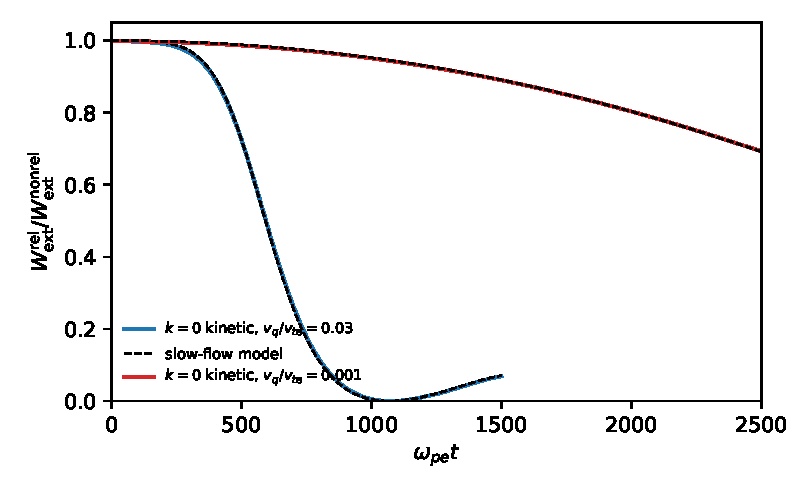
\includegraphics[width=0.78\linewidth]{figures/fig_cold_relativistic.pdf}
\caption{Ratio of the external work of the relativistic to the nonrelativistic homogeneous plasma under a resonant uniform drive (solid), from the $k=0$ Vlasov equation integrated with 48 Gauss--Hermite momentum nodes and cold ions with $m_i/m_e=1836$, and the slow-flow model with the thermal term (black dashed). Generated by \texttt{note/make\_note\_figures.py}.}\label{fig:relcold}
\end{figure}

We checked this with a calculation of our own that is exact for the homogeneous collisionless problem (script \texttt{note/make\_note\_figures.py}, output \texttt{note/figures/k0\_relativistic.json}; it is a calculation made for this note and not a study record, and it is the reference for the relativistic timing in Chapters~\ref{ch:model} and~\ref{ch:rel}): the relativistic Vlasov equation at $k=0$, in which every electron momentum evolves as $\dot p=-F(t)$ with the common force field $F$, the current is the Maxwellian average of $p/\gamma$ over the initial momentum (48 Gauss--Hermite nodes, exact for this smooth integrand to far better than the quantities quoted), and the ions are cold. Its external work departs from the nonrelativistic linear resonant law by 10\,\% at $\wpe t=392.3$ for $\vq=0.03$, against $392.5$ for the relativistic Hermite record (paper, relativistic section; \texttt{studies/relhhs/summary.json}). For $\vq=10^{-3}$ it gives $1428.8$, against $1309.5$ and $1413.5$ for the deterministic and the shot-noise relativistic grid (\texttt{studies/relgrid/summary.json}); the slow-flow model gives $397$ and $1438$. The cold model alone gives $437$ for the strong drive, and for the weak drive it does not collapse in the time of interest, which is why the thermal term is needed; the figure shows the kinetic and slow-flow results with the thermal term. We do not draw from this agreement that the detuning is the whole story of the paper's collapse time, since the continuum models include $k\neq0$ modes; but it shows that the timing of the collapse in the paper is accounted for by the homogeneous physics that nonrelativistic models cannot contain, and that no nonlinear inhomogeneous process is needed for it. This is the finding (i) of the paper's abstract. The Jüttner distribution, the relativistic equilibrium
\begin{equation}
f_J(\bp)\propto\exp\!\Big[-\frac{\gamma(p)\,mc^2}{T}\Big] ,
\end{equation}
introduced by J\"uttner~\citep{Juttner1911}, reduces to the Maxwellian when $T\ll mc^2$; in one momentum dimension its normalization is $\int\ee^{-\gamma/\theta}\dd p=2K_1(1/\theta)$ with $\theta=T/mc^2$ and $K_1$ the modified Bessel function, because with $p=\sinh s$ the integral is $2\int_0^\infty\ee^{-\cosh s/\theta}\cosh s\,\dd s$. It is the right initial condition when the electrons have been heated above a few per cent of $mc^2$.

\chapter{Numerical methods for the Vlasov--Maxwell--Proca system}\label{ch:numerics}

Chapter~\ref{ch:plasma} gave the analytic yardsticks; the numerical methods that must reproduce them come next. The paper compares four kinds of calculation: a particle-in-cell code, a semi-Lagrangian grid solver, a Hermite spectral solver in velocity, and the analytic theory of Chapters~\ref{ch:darkphoton} and~\ref{ch:plasma}. A reader who has used one family of methods tends to take for granted what the others do badly, and the conclusions of the paper depend on exactly those differences: a particle method has shot noise but no positivity problem, a spectral method has the reverse, and a grid method pays in memory for what it saves in noise. This chapter describes the methods in enough detail to make that statement precise, and then the architecture of Dark-SPECTRAX that implements the Hermite--Fourier one.

\section{Particle-in-cell}\label{sec:pic}

A particle-in-cell code represents the distribution function by a finite number of macroparticles, $f_s(x,v,t)\simeq\sum_pw_p\,\delta(x-x_p(t))\,\delta(v-v_p(t))$, each carrying a weight $w_p$ (number of physical particles) and moving along the characteristics of the Vlasov equation. The fields live on a grid. The method was developed in the 1960s and 1970s, and the standard references are the books by Birdsall and Langdon~\citep{BirdsallLangdon1985} and Hockney and Eastwood~\citep{HockneyEastwood1988} and the review by Dawson~\citep{Dawson1983}. A step has four parts: deposit charge and current from particles onto the grid, advance the fields, interpolate the fields back to the particles, and push the particles.

The grid enters through a shape function $S$. Each macroparticle is a finite-size cloud, and the charge density at node $x_j$ is $\rho_j=\sum_pq_pw_p\,S(x_j-x_p)/\Delta x$, with $\int S=1$. Using for $S$ the B-splines of order $m$ gives nearest-grid-point ($m=0$), cloud-in-cell ($m=1$), triangular-shaped cloud or quadratic ($m=2$) and the higher-order variants, up to the quintic splines ($m=5$) used by HHS. The field is interpolated to the particle with the same shape, $E(x_p)=\sum_jE_jS(x_j-x_p)$, because with identical deposition and interpolation the discrete force between two particles is antisymmetric and total momentum is conserved (the analogue of Newton's third law). Finite-size particles also change the dynamics: their Fourier transform $\hat S(k)$ multiplies the effective coupling, which reduces the strength of collisions at scales below the cloud size and damps the high-$k$ structure of the noise~\citep{LangdonBirdsall1970}. A higher-order shape is smoother and noisier at the grid scale only through the aliasing of $k$ components beyond the Nyquist wave number, so raising the order trades a larger stencil for a cleaner spectrum.

Maxwell's equations are advanced with a Yee-type staggered scheme, and the current must be deposited so that the discrete continuity equation holds, $\partial_t\rho_j+(J_{j+1/2}-J_{j-1/2})/\Delta x=0$, otherwise Gauss's law drifts. Villasenor and Buneman gave a charge-conserving deposition for first-order shapes~\citep{VillasenorBuneman1992}, and Esirkepov generalized it to arbitrary shape~\citep{Esirkepov2001}. In one dimension the construction is elementary: the current through a cell face is the change in the cumulative shape function that crosses the face during the step. A scheme that does not do this must correct the electric field with a Poisson solve.

The particle push for a relativistic particle uses $\bu=\gamma\bv$. The Boris algorithm~\citep{Boris1970} splits the Lorentz force $\dd\bu/\dd t=(q/m)(\bE+\bu\times\bB/\gamma)$ into two half-accelerations by the electric field and one rotation by the magnetic field:
\begin{align}
\bu^-&=\bu^{n}+\frac{q\Delta t}{2m}\bE ,\qquad \gamma^-=\sqrt{1+|\bu^-|^2/c^2},\\
\bu'&=\bu^-+\bu^-\times\mathbf t ,\qquad \bu^+=\bu^-+\bu'\times\frac{2\mathbf t}{1+t^2} ,\qquad\mathbf t=\frac{q\Delta t}{2m\gamma^-}\bB ,\\
\bu^{n+1}&=\bu^++\frac{q\Delta t}{2m}\bE .
\end{align}
The rotation preserves $|\bu|$ exactly, so the magnetic field does no work at any step size, and the map is volume preserving, which is why Boris is the default in codes that must run for very many steps. The rotation angle $\theta$ satisfies $\tan(\theta/2)=t$, a phase error of second order in $\Delta t$. In the relativistic limit Boris has a known flaw: in crossed $\bE$ and $\bB$ fields with $|\bE|\simeq c|\bB|$ the force on a particle that is moving at constant velocity does not cancel to the required accuracy, because the average of $\bv$ is taken at the half step with a $\gamma$ computed from the intermediate momentum. Vay proposed to evaluate the magnetic force with the average of the old and new velocities and solve the resulting implicit equation in closed form~\citep{Vay2008}. In his scheme one computes $\bu'=\bu^n+(q\Delta t/m)(\bE+\bv^n\times\bB/2)$ and then
\begin{equation}
\gamma_{n+1}^2=\tfrac12\Big(\sigma+\sqrt{\sigma^2+4(\tau^2+u_*^2)}\Big),\quad
\bu^{n+1}=\frac{\bu'+(\bu'\!\cdot\!\mathbf t)\mathbf t+\bu'\times\mathbf t}{1+t^2},
\end{equation}
with $\boldsymbol\tau=q\Delta t\bB/2m$, $\sigma=\gamma'^2-\tau^2$, $u_*=\bu'\cdot\boldsymbol\tau/c$ and $\mathbf t=\boldsymbol\tau/\gamma_{n+1}$. Both pushers reduce to the same thing in the electrostatic one-dimensional problem of this note, where $\bB=0$ and the push is the second-order leapfrog; the relevance of the choice to HHS is that they use the Vay algorithm, which we cannot vary in a code without a magnetic field.

The sampling error is the defining property of the method. If a cell of width $\Delta x$ holds $N_{\rm ppc}$ macroparticles, the density fluctuates by $\delta n/n\sim N_{\rm ppc}^{-1/2}$, so the PIC error converges as $N^{-1/2}$ unless the particles are loaded in a quiet start. The fluctuations drive electric fields: in electrostatics $E_k=\ii e\,\delta n_k/(\epsilon_0k)$, so the energy density of the noise in a cell is $\sim\tfrac12nT\,(\Delta x/\lDe)^2/N_{\rm ppc}$ (this estimate is ours, from $k\sim1/\Delta x$ and $\delta n^2/n^2=1/N_{\rm ppc}$). For the HHS set-up, $\Delta x=0.04\,c/\wpe$ and $\lDe=0.0316\,c/\wpe$, so the noise energy is about $1.6/N_{\rm ppc}$ times $\tfrac12nT=\Eth$; with the ladder of 103 to 1648 particles per cell of the paper this is $1.6\times10^{-2}$ to $10^{-3}$ of $\Eth$, small compared with the heating reported (tens of $\Eth$). The noise is nevertheless not innocuous. It seeds every unstable mode at a finite amplitude, which a deterministic code does not have unless it is given one, and the paper's central open question is whether this seed, and not a deterministic mechanism, produces the heating (Sec. ``Continuum methods against the PIC heating'' of the paper). The PIC has no positivity problem: the distribution is a sum of delta functions weighted positively.

Energy conservation in explicit PIC is only approximate. The scheme conserves momentum exactly, with matched shapes, but the energy changes by an amount that is second-order in $\Delta t$ and depends on the grid: when $\Delta x$ is larger than a few Debye lengths, aliased modes heat the plasma secularly, the finite-grid instability analyzed by Langdon and Birdsall~\citep{LangdonBirdsall1970}. Implicit schemes can conserve energy and charge simultaneously at the price of a nonlinear solve per step, as shown by Chen, Chac\'on and Barnes~\citep{ChenChacon2011} and by Markidis and Lapenta~\citep{MarkidisLapenta2011}. HHS use SHARP, a relativistic PIC code with a spatially higher-order discretization~\citep{Shalaby2017}, with fifth-order spline functions in deposition and interpolation, the Vay pusher, and between $2\times10^2$ and $2\times10^5$ particles per cell (Supplemental Material, Sec.~II of Ref.~\citep{HHS2026}). The independent relativistic PIC of the paper is built on Dark-JAX-in-Cell~\citep{DarkJIC}, with quadratic shapes by default and a quintic test. At $\vq=0.03$ the paper's electron heating at $\wpe t=1000$ converges to a plateau of about 25 initial thermal energies, with changes of 1.4\% and 0.1\% for each doubling of particles from 412 to 1648 per cell and 0.8\% when the cell is halved from $0.02$ to $0.01\,c/\wpe$ (paper, Table on PIC convergence). Dark-JAX-in-Cell was also used to check the Landau damping of the Hermite model: at 128 cells and 320\,000 particles the fitted frequency and damping agree within 0.1\% and 1\% (README, comparison with Dark-JAX-in-Cell), a measure of what the PIC needs to match a noise-free solver at $k\lDe=0.5$.

\section{Continuum methods: grids and discontinuous Galerkin}\label{sec:grid}

A continuum method represents $f$ on a grid in phase space, or by an expansion in basis functions, and has no sampling noise. Its costs are the curse of dimensionality (a six-dimensional grid for the full problem) and the need to keep $f$ positive and well resolved when it develops fine structure.

The semi-Lagrangian approach advances $f$ along characteristics over a time step and interpolates back to the grid. For the Vlasov--Poisson system the operator splitting of Cheng and Knorr~\citep{ChengKnorr1976} alternates a shift in $x$ by $v\Delta t$ and a shift in $v$ by $E\Delta t$; each is an exact translation, which makes the scheme second order, unconditionally stable in the translation steps (no CFL condition) and cheap, and with a spectral interpolation each shift is exact for band-limited data. The comparison of Eulerian solvers by Filbet and Sonnendr\"ucker~\citep{FilbetSonnendrucker2003} remains a good guide to the properties of this class, and Einkemmer and Ostermann gave the convergence analysis of Strang splitting for Vlasov-type equations~\citep{Einkemmer2014}. For the Vlasov--Maxwell system, Crouseilles, Einkemmer and Faou proposed a Hamiltonian splitting that handles the magnetic terms with a sequence of sub-steps that are each exactly solvable~\citep{Crouseilles2015}. The repository uses a NumPy semi-Lagrangian Vlasov--Poisson solver, extended to Vlasov--Amp\`ere--Proca for the dark runs, as an independent reference that shares no code with SPECTRAX (README, independent grid codes), and a relativistic momentum-space grid solver of the same family for the relativistic checks of the paper. In the relativistic grid, the momentum grid has 4096 nodes and $N_x=32$ Fourier modes (paper, Sec. on the relativistic extensions).

Discontinuous Galerkin methods approximate $f$ element by element with polynomials of fixed degree and couple elements by numerical fluxes. They are high order, local and conservative, and have been developed for kinetic equations in a series of works by Juno, Hakim and collaborators~\citep{Juno2018}; for the relativistic Vlasov--Maxwell system, Juno et al.\ recently built a conservative DG scheme with a velocity-space mapping that deals with the wide range of energy scales in relativistic plasmas, and describe its noise-free character as the point of the method~\citep{Juno2026}. This is the nearest neighbour to our relativistic grid and to the relativistic Hermite option in the sense that it addresses the same physics (relativistic kinetics without Poisson noise), but over a different basis.

Table~\ref{tab:methods} summarizes the properties that decide the choice for the problem at hand. The entries are qualitative and refer to the schemes described above, in their standard form; each can be modified, and the references show how.

\begin{table}[t]
\centering
\caption{Qualitative comparison of the methods in the standard forms described in this chapter. ``Noise'' is sampling noise in the distribution function. ``Positivity'' is whether $f\ge0$ is guaranteed by the discretization.}\label{tab:methods}
\small
\begin{tabular}{@{}p{3.2cm}p{1.6cm}p{2.3cm}p{3.5cm}p{3.4cm}@{}}\toprule
Method & Noise & Positivity & Invariants (semi-discrete) & Main cost driver\\\midrule
PIC, explicit & yes, $N_{\rm ppc}^{-1/2}$ & yes (weights $>0$) & momentum; energy only to $O(\Delta t^2)$, grid heating & particles per cell, steps\\
PIC, implicit energy-conserving & yes & yes & charge and energy & nonlinear solve per step\\
Semi-Lagrangian grid & no & not guaranteed (interpolation) & mass; energy approximately & phase-space grid points\\
DG in phase space & no & not guaranteed (limiters help) & mass, energy with central fluxes & elements $\times$ degree$^{d}$\\
Hermite, AW & no & no & mass, momentum, and energy up to closure; AW Galerkin instability & Hermite order, step $\propto1/\sqrt{N_n}$\\
Hermite, SW & no & only in the square-root form & $L^2$ norm; no closure conserves all three moments & Hermite order\\\bottomrule
\end{tabular}
\end{table}

\section{Spectral discretization in velocity: the Hermite expansion}\label{sec:hermite}

The velocity space of a plasma close to a Maxwellian is well represented by a short expansion in Hermite functions, and a spectral method turns the Vlasov equation into a hierarchy of equations for the expansion coefficients, which are moments of the distribution. Grad's moment method of 1949 is the antecedent~\citep{Grad1949}, Fourier--Hermite expansions were applied to the Vlasov equation from the 1960s, and Holloway's analysis of spectral velocity discretizations~\citep{Holloway1996} and the velocity-scaled Hermite simulations of Schumer and Holloway~\citep{SchumerHolloway1998} gave the theory and practice that most of the modern work follows. The modern revival, driven by exascale hardware and by the demand for noise-free kinetic simulation, includes the fully implicit scheme of Delzanno with exact discrete conservation~\citep{Delzanno2015}, the comparison of Camporeale et al.\ with PIC~\citep{Camporeale2016}, the three-dimensional Hermite--DG code of Koshkarov et al.~\citep{Koshkarov2021} and the analysis of its conservation properties and time integrators by Pagliantini et al.~\citep{Pagliantini2023a}.

We write the expansion in one velocity dimension; the three-dimensional case is a tensor product. Let $\xi=(v-u)/a$, with width $a$ and shift $u$ to be chosen. The \emph{asymmetrically weighted} (AW) basis, used by the parent solver SPECTRAX, is
\begin{equation}
f(x,v,t)=\sum_{n=0}^{N-1}C_n(x,t)\,\Psi_n(\xi),\qquad \Psi_n(\xi)=\frac{H_n(\xi)\,\ee^{-\xi^2}}{\sqrt{\pi\,2^n\,n!}} ,\label{eq:AW}
\end{equation}
where $H_n$ are the physicists' Hermite polynomials. The functions are orthogonal with respect to the weight $\ee^{+\xi^2}$ and not $\ee^{-\xi^2}$, hence the name: the Gaussian factor appears once in the basis function and the weight is the inverse Gaussian. The coefficients are moments: since $\int\Psi_nH_m\,\dd\xi=\sqrt{2^nn!}\,\delta_{nm}$,
\begin{equation}
C_n=\frac{1}{a\sqrt{2^nn!}}\int f\,H_n\!\Big(\frac{v-u}{a}\Big)\dd v .
\end{equation}
The density is $\int f\,\dd v=aC_0$, the particle flux is $\int vf\,\dd v=a\,(uC_0+aC_1/\sqrt2)$, and the second moment involves $C_2$. Number, momentum and energy are therefore the first three coefficients, and the current that sources Amp\`ere's law is a linear function of $C_1$ (and $C_0$ in a shifted basis), which is why the field solve costs nothing.

The Hermite polynomials satisfy $\xi H_n=\tfrac12H_{n+1}+nH_{n-1}$ and $H_n'=2nH_{n-1}$; from them, the ladder relations of the AW basis are
\begin{equation}
\xi\Psi_n=\sqrt{\tfrac{n+1}{2}}\,\Psi_{n+1}+\sqrt{\tfrac n2}\,\Psi_{n-1},\qquad \partial_\xi\Psi_n=-\sqrt{2(n+1)}\,\Psi_{n+1} .\label{eq:ladder}
\end{equation}
The first holds because $\xi$ multiplies $H_n$ and the normalization $1/\sqrt{\pi2^nn!}$ turns $\tfrac12H_{n+1}$ into $\sqrt{(n+1)/2}$ times the normalized $\Psi_{n+1}$; the second follows from $\partial_\xi(H_n\ee^{-\xi^2})=(2nH_{n-1}-2\xi H_n)\ee^{-\xi^2}=-H_{n+1}\ee^{-\xi^2}$. Insert $v=u+a\xi$ in the one-dimensional Vlasov equation, project on the basis and use Eq.~\eqref{eq:ladder}. In the Fourier representation in $x$ the result is
\begin{equation}
\partial_tC_n+\ii k\Big[u\,C_n+a\sqrt{\tfrac{n+1}{2}}\,C_{n+1}+a\sqrt{\tfrac n2}\,C_{n-1}\Big]=\frac{q}{ma}\sqrt{2n}\;\big(E\ast C_{n-1}\big) ,\label{eq:hierarchy}
\end{equation}
with $\ast$ the convolution in $k$ that represents the product $E(x)C_{n-1}(x)$. The streaming term couples neighbouring orders through the symmetric tridiagonal matrix $T$ with entries $T_{n,n\pm1}=\sqrt{(n+1)/2}$ or $\sqrt{n/2}$; its eigenvalues are the nodes of the Gauss--Hermite quadrature, the largest being about $\sqrt{2N}$. The force term only moves information from lower to higher $n$: it is strictly lower triangular in the Hermite index. This structure explains most of the numerical behaviour of the method.

Consider free streaming from a basis-matched Maxwellian, $f_1=\ee^{-\ii kvt}f_M(v)$ with $a=\sqrt2\vte$. Then $C_n=\int\ee^{-\ii s\xi}H_n(\xi)\ee^{-\xi^2}\dd\xi/(\sqrt\pi\sqrt{2^nn!})$ with $s=kat$, and the identity $\int H_n\ee^{-\xi^2-\ii s\xi}\dd\xi=\sqrt\pi(-\ii s)^n\ee^{-s^2/4}$ gives $|C_n|^2=(k\vte t)^{2n}\ee^{-(k\vte t)^2}/n!$. The spectrum in $n$ is a Poisson distribution with mean $(k\vte t)^2$: the information flows up the ladder at the rate with which the velocity structure $\ee^{-\ii kvt}$ becomes finer, and a truncation at $N$ is accurate until $(k\vte t)^2\sim N$, that is, $t\sim\sqrt N/(k\vte)$. After this time the truncated system reflects the wave at the end of the ladder and the solution recurs. This is the Hermite counterpart of the recurrence in a velocity grid with spacing $\Delta v$, which occurs at $t=2\pi/(k\Delta v)$. The fix in both cases is dissipation at the small scales, which in the Hermite case is a damping that acts on high $n$.

The closure problem is the question of what to set for $C_N$ in the equation for $C_{N-1}$. Truncation, $C_N=0$, reflects; the choices in use are filters, hypercollisions and Landau-fluid closures. Hammett and Perkins constructed a closure from the linear response that reproduces Landau damping with a few fluid moments~\citep{HammettPerkins1990}. Hypercollisions add $-\nu\,s(n)C_n$ with $s(n)\propto n^p$, sometimes with a floor so that the first conservation orders are not touched; the parent solver uses $s(n)\propto n(n-1)(n-2)$, which leaves $n=0,1,2$ (density, momentum, energy) unchanged. Parker and Dellar showed how the free energy flows up the ladder in linear Landau damping and back down in the nonlinear case, which is the physical picture behind a closure that must not reflect~\citep{ParkerDellar2015}. Camporeale et al.\ added an artificial collisional operator for the filamentation problem~\citep{Camporeale2016}, and Issan et al.\ compared artificial collisions, exponential filters and nonlocal closures in a systematic study of the effect on Landau damping, nonlinear Landau damping and the two-stream instability~\citep{Issan2025}. For the paper we use a hypercollision whose strength is scaled by the maximum electric field,
\begin{equation}
\nu_s=c\Big|\frac{q}{m}\Big|_s\frac{\sqrt{2N_n}\,\max|E-\langle E\rangle|}{a_s}\;\frac{n(n-1)(n-2)}{(N_n-1)(N_n-2)(N_n-3)},
\end{equation}
so that the rate at the top of the ladder equals $c$ times the Hermite-space velocity (in $n$ per unit time) at which the force carries information up the ladder (paper, Sec. on closures).

The alternative to the AW basis is the \emph{symmetrically weighted} (SW) basis $\varphi_n=H_n\ee^{-\xi^2/2}/\sqrt{\sqrt\pi\,2^nn!}$, orthonormal in $L^2$. Its ladder relations are $\xi\varphi_n=\sqrt{(n+1)/2}\,\varphi_{n+1}+\sqrt{n/2}\,\varphi_{n-1}$ and $\partial_\xi\varphi_n=\sqrt{n/2}\,\varphi_{n-1}-\sqrt{(n+1)/2}\,\varphi_{n+1}$, so that the discretized force term is an antisymmetric tridiagonal matrix times $E(x)$. A skew-symmetric Galerkin operator conserves the discrete $L^2$ norm of $f$ and cannot have exponentially growing modes. The price is that the SW expansion does not preserve the simple moment structure of AW, and its conservation of momentum and energy requires closures that Issan et al.\ show cannot simultaneously conserve the three invariants~\citep{Issan2024b}. The antisymmetric formulation, with the square-root transformation that also preserves positivity, is the subject of Ref.~\citep{Issan2024a}. Bessemoulin-Chatard and Filbet proved weighted-$L^2$ stability, and conservation of mass, momentum and energy, for the Hermite spectral form with a time-dependent weight~\citep{BessemoulinChatardFilbet2021}. A mixed Hermite--Legendre method that uses Legendre polynomials for localized features such as beams and plateaus is proposed in Ref.~\citep{Issan2026}, and a recent Galerkin method with AW functions that is designed to be stable is that of Dai~\citep{Dai2026}.

The distinction is not academic here, because the AW basis, which the parent solver uses and which makes the pump-frame remap exact, has a numerical instability. In a spatially varying field the frozen-field spectrum of the AW Galerkin operator $-\ii kaT+(q/ma)\sqrt{2n}\,E$ has modes that grow, concentrated in the top third of the ladder: the streaming matrix is real symmetric and the force matrix is strictly lower triangular and nilpotent, so neither has an eigenvalue with positive real part, but their sum is a non-normal matrix, and the product of upward and downward couplings can produce growth. At $K=5$ Fourier modes, $N_n=128$ and field amplitude $E_1=10^{-2}$ the largest growth rate is $1.6$ for the AW basis against $8\times10^{-15}$ (round-off) for the SW basis (\texttt{studies/highk/eig.json}, paper Fig.~2). The growth rate rises with $N_n$, which means that refining the velocity basis moves the end of the run earlier, and this defines the certified windows of the nonrelativistic paper: $1000$, $892$ and $791.5$ at $\vq=0.03$, $0.05$, $0.07$. The paper and the design note record the routes tried to remove the instability (stronger closure, GPU resolution, the SW basis and a square-root form) and why they failed under the declared gates; for the purpose of this chapter the point is that a Hermite basis can be energetically fine in a continuous sense and unstable in a discrete one, and the choice among bases is a choice of which defect to live with.

\section{Scaling, shifting and adaptivity}\label{sec:scaling}

The width $a$ and shift $u$ in Eq.~\eqref{eq:AW} are free parameters of the discretization. A basis that does not match the distribution needs many more terms, because the Hermite functions are orthogonal for one Gaussian only. Tang observed that the standard normalized Hermite functions require too many terms for Gaussian-type functions unless a scaling factor is chosen, and gave the factor in terms of the largest root of $H_{N+1}$~\citep{Tang1993}. Ma, Sun and Tang made the scaling depend on time to follow the spreading of the solution of a parabolic equation in an unbounded domain, and proved convergence~\citep{MaSunTang2005}. Schumer and Holloway introduced a variable velocity scale into the Hermite basis for the one-dimensional Vlasov--Poisson system and found errors reduced by orders of magnitude at no increase in workload~\citep{SchumerHolloway1998}; they also compared the two weightings and noted that the AW basis conserves particles and momentum exactly but not the square integral of $f$, and is numerically unstable, while the SW basis conserves the square integral (this is the instability that reappears in the next section and in the paper)~\citep{SchumerHolloway1998}. Fatone et al.\ studied the dependence on the scaling parameter in a semi-Lagrangian spectral Vlasov--Poisson scheme and concluded that the parameter should be updated during the computation~\citep{Fatone2018}. Pagliantini, Delzanno and Markidis designed the adaptivity: after each time step a criterion sets $a$ and $u$ from the bulk velocity and temperature of each species, and a map between the approximation spaces of different parameters preserves mass, momentum and energy; the resulting method has fluid--kinetic coupling, since the lowest coefficients become the fluid moments~\citep{Pagliantini2023b}.

The AW basis makes the remap simple. The coefficients with respect to a new pair $(u',a')$ are $C_m'=(a'\sqrt{2^mm!})^{-1}\int f\,H_m((v-u')/a')\,\dd v$, and $H_m((v-u')/a')$ is a polynomial of degree $m$ in $\xi=(v-u)/a$. Hence $C_m'$ is a linear combination of the moments $\int f\,\xi^j\,\dd v$ with $j\le m$, which are combinations of $C_0,\dots,C_j$: \emph{the remap is lower triangular}, $C'_m=\sum_{n\le m}R_{mn}C_n$, with no error for any $m<N$ when the lower coefficients are exact. In particular every moment below the truncation order is preserved exactly. The SW basis has no such property: the change of the Gaussian weight is not a polynomial map and mixes all orders. This is the reason why the model's ``pump frame'' uses AW functions: in the resonant calculation, each species oscillates with a coherent velocity $u_s(t)$ that grows to $0.5c$, and the centre follows the total uniform force, $\dot u_s=(q/m)_s(\bar{\bf E}+u_s\times\bar{\bf B})$ with the box averages including the dark field and the drive. This is an exact change of variables (the kernel receives $E-\bar E$), so the coherent $k=0$ quiver is carried by $u_s(t)$ and not by the high orders of the Hermite ladder, which would have to represent a displaced Gaussian by an enormous number of terms. Widths and residual drifts change only between integration segments, through the triangular remap, with the triggers and caps recorded in the repository ($|U-u|/a>0.3$ or $|a'/a-1|>0.05$; $|\Delta u|\le a'$; $a/a'\le1.1$).

\section{Fourier pseudo-spectral discretization in space}\label{sec:fourier}

In space the periodic box is discretized by a Fourier series, and products such as $E(x)C_{n-1}(x)$ in Eq.~\eqref{eq:hierarchy} are computed pseudo-spectrally: transform to the grid, multiply pointwise and transform back. The product of two fields with wave numbers $|m_1|,|m_2|\le M$ has wave numbers up to $2M$, and on a grid of $N_x$ points a wave number $p$ is indistinguishable from $p-N_x$. If all modes with $|m|\le M$ are retained, a product term at $p>N_x-M$ is aliased into a retained mode. Requiring that no product mode of order $2M$ alias into a retained mode, $2M<N_x-M$, gives $M<N_x/3$: the $2/3$ rule of Orszag~\citep{Orszag1971}, which discards the upper third of the spectrum and makes quadratic products exact. The parent applies a mask retaining modes with $3|m|<N_x$ (a ``strict'' $2/3$ rule, after SPECTRAX pull request 55), so that every grid size, including multiples of 3, is free of aliasing for quadratic products. The dealiased method is spectrally accurate for smooth fields; for the Vlasov equation the discretization in $x$ is not the limiting factor in the cases of interest, since the high-$k$ content of the fields is small or physically relevant (the OTSI cascade reaches large $k$ and drives the choice of $N_x$ in the paper).

A real field requires only $k\ge0$ (the real FFT), and the box average is a weighted sum over this half spectrum with weight 1 for $k=0$ (and for the Nyquist mode when $N_x$ is even) and 2 otherwise. This is how the energy ledger is evaluated from the stored coefficients without returning to the grid.

The two discretizations together set the cost of a run, and the numbers can be estimated before running. In the HHS box, $L=40\,c/\wpe$ and $\lDe=\vte/\wpe=0.0316\,c/\wpe$, so a wave number $k\lDe=1$ is $k=31.6\,\wpe/c$, which is the Fourier mode $m=kL/2\pi\simeq201$. With the $2/3$ rule the grid must have at least $3m\simeq604$ points to resolve that mode without aliasing, so $N_x=32$, $64$ and $128$ retain modes up to $m=10$, $21$ and $42$ and cover $k\lDe$ up to about $0.05$, $0.10$ and $0.21$, while $N_x=1024$ reaches $m=341$ and $k\lDe\simeq1.7$. The Hermite order needed for a collisionless linear phase-mixing problem up to the time $T$ is $N_n\gtrsim(k\vte T)^2$ from the Poisson spectrum of Eq.~\eqref{eq:hierarchy} (for $k\lDe=0.3$ and $\wpe T=100$ this is $\simeq900$, the order of the $N_n=512$ to $1024$ used for nonlinear Landau damping in the repository, and for $k\lDe=1$ and $\wpe T=1000$ it is $10^6$, which is why closures and collisions are needed and why the solution is only trusted until the first disagreement between orders). The cost of a PIC run scales as $N_xN_{\rm ppc}N_t$ with a noise error $\propto N_{\rm ppc}^{-1/2}$, while the Hermite run scales as $N_xN_nN_t$ with an error that decays exponentially in $N_n$ for smooth data until the filamentation reaches the end of the ladder. The comparison of Camporeale et al.\ shows the consequence: for the smooth problems of their study the Hermite method reached solutions several orders of magnitude more accurate at a fraction of the cost of PIC~\citep{Camporeale2016}. Our problem differs by being strongly nonlinear with an instability cascade to small scales, so that the Hermite advantage is not a given; the certified windows of the paper are the measure of how far it holds.

\section{Time integration}\label{sec:time}

The semi-discrete system is a large system of ordinary differential equations $\dot y=f(t,y)$ with a stiff and a nonstiff part. Streaming has imaginary eigenvalues $\pm\ii kax_j$, with $x_j$ the Gauss--Hermite nodes up to $\sqrt{2N_n}$, so the stable step of an explicit method decreases as $1/(K\sqrt{N_n})$. This is the CFL condition of the spectral method, and it is the cost of high resolution in $n$. The closure damping is real and negative with magnitude up to its strength, and is stiff only for strong closures.

The default integrator of Dark-SPECTRAX is the eighth-order explicit Runge--Kutta method Dopri8 of the Diffrax library~\citep{Kidger2021}, with embedded error estimation and a proportional-integral-derivative step-size controller that adjusts the step to a relative tolerance $10^{-10}$ and an absolute tolerance $10^{-12}$. A high order is appropriate because the problem is smooth, the cost per step is eight right-hand-side evaluations with a single FFT of the fields, and it is the integrator error and not the spatial or velocity truncation that we want to be negligible. The work ledger is integrated as additional variables with the same stages, so that $K-K_0=W_\gamma+W_D+\Wext$ is a statement about the integrator and closes to the solver tolerance.

The implicit midpoint rule is a different tool for a different purpose. For $\dot y=f(y)$ it reads $y_{n+1}=y_n+\Delta t\,f\big(\tfrac12(y_n+y_{n+1})\big)$. It is second-order, A-stable and symmetric, and it conserves every quadratic invariant of the continuous system. To see this, suppose $y^{\rm T}Qy$ is invariant with $Q$ symmetric, so that $y^{\rm T}Qf(y)=0$ for all $y$. Then $y_{n+1}^{\rm T}Qy_{n+1}-y_n^{\rm T}Qy_n=(y_{n+1}-y_n)^{\rm T}Q(y_{n+1}+y_n)=2\Delta t\,f(\bar y)^{\rm T}Q\bar y=0$ with $\bar y=\tfrac12(y_n+y_{n+1})$. For the Vlasov--Poisson and Vlasov--Maxwell systems in the Hermite representation the discrete energy and, in the SW basis, the $L^2$ norm are quadratic, so the midpoint rule conserves them exactly, which is the reason why implicit second-order schemes of this type (Crank--Nicolson, which is the midpoint rule for these equations) are used by Delzanno~\citep{Delzanno2015}, Issan et al.~\citep{Issan2024a} and Pagliantini et al.~\citep{Pagliantini2023b}. The parent solver provides it as a Diffrax solver with a Newton--GMRES nonlinear solve, and the cost is that of a nonlinear solve per step, not eight right-hand sides. Pagliantini et al.\ analyze when explicit methods, with relaxation, can preserve energy instead~\citep{Pagliantini2023a}.

When the stiffness comes from a known linear part the exponential integrators remove it from the stability restriction. Write $\dot y=Ay+g(t,y)$ with $A$ the stiff operator. Lawson's integrating-factor method sets $z=\ee^{-tA}y$, so that $\dot z=\ee^{-tA}g(t,\ee^{tA}z)$, and advances $z$ with an explicit Runge--Kutta method; for the linear test problem the stiffness is removed exactly and the explicit method sees only $g$~\citep{Lawson1967}. Cox and Matthews gave exponential time differencing as the other principal family~\citep{CoxMatthews2002}, and Hochbruck and Ostermann reviewed both, including the rate of convergence for semilinear problems~\citep{Hochbruck2010}. The review makes a point that matters here: for stiff problems the classical order is not always attained, and the Lawson--Runge--Kutta schemes are of lower stiff order than their nonstiff order. The effective order depends on the ratio of the step to the stiff time scale, and one should not claim the full order of Dopri8 when the closure rate times the step is large. For kinetic equations, Crouseilles, Einkemmer and Massot studied exponential integrators for collisionless kinetic equations, whose linear part (free streaming) is exactly solvable in Fourier space and removes the CFL condition. They showed that classic exponential integrators behave erratically in the step size they allow, and that Lawson methods do not suffer from this, which they demonstrated on the Vlasov--Poisson system and a drift-kinetic model~\citep{Crouseilles2020}.

In Dark-SPECTRAX the stiff part is the diagonal closure, $A=-\mathrm{diag}(r)$, which is exactly exponentiable. For $c=64$ the Jacobian's spectral radius equals the closure rate to the printed precision, and the Lawson wrapper around Dopri8 reduces the number of steps by a factor of $5.0$ to $\wpe t=500$ with $\Delta K_e$ and $\Wext$ agreeing with the plain integration to $5\times10^{-10}$; for $c=4$ the closure is not stiff and the step ratio is $0.96$ (\texttt{studies/expint/summary.json}). An exact streaming factor in the same framework gave no step reduction and cost 2.7 times more per step. The gain is real but it is not the limit of the method: the largest real part of the eigenvalues of the instability is 2--3, smaller than the closure rate, so the time step is not controlled by the instability (paper, failed-checks table).

\section{Architecture of Dark-SPECTRAX}\label{sec:architecture}

Dark-SPECTRAX is a Python package of about a thousand lines that adds the Proca sector, the prescribed drive, the work ledger, the pump-frame logic, a relativistic option and the study tooling to the Hermite--Fourier kernel of the parent solver SPECTRAX~\citep{SPECTRAX}. The parent is a JAX code, so that the right-hand side is a pure function of a state pytree, can be compiled with XLA, run on CPU or GPU, and differentiated. Dark-SPECTRAX keeps the parent as a dependency, pinned to a commit on an integration branch (the commit is recorded in each study record), and calls it through a small adapter section of one module; its own files are the model (configuration and right-hand side), the simulation drivers, the closure and the streaming factor, and the diagnostics.

The state is a dictionary of complex arrays. The Hermite coefficients are stored as \texttt{Ck} with shape $(N_sN_nN_mN_p,\;N_y,\;N_x/2+1,\;N_z)$: the first axis is the flattened species and Hermite index, $N_n,N_m,N_p$ being the numbers of Hermite orders in the three velocity directions, with the parent storage order $(p,m,n)$ in the Hermite index; the spatial axes are the real-FFT layout, with the half spectrum along $x$. The ordinary fields are \texttt{Fk} of shape $(6,\dots)$ for $\bE$ and $\bB$ in the same Fourier layout; the dark fields are \texttt{Dk} of shape $(10,\dots)$ for $\ED$, $\BD$, $\AD$ and $\phiD$; \texttt{W} holds the three works; and in the pump frame \texttt{B} holds the centres and widths $(u_s,a_s)$ as variables that evolve. All state is complex because the parent keeps its Fourier coefficients complex; the ledger variables are stored as complex with zero imaginary part because Diffrax requires one dtype across the Runge--Kutta stage buffers.

The right-hand side \texttt{rhs(t, y, model)} has one structure for all modes. The physical force fields are synthesized from \texttt{Fk} (plus $\eta\,$\texttt{Dk} in the self-consistent mode, plus the drive in the prescribed mode), multiplied by the dealiasing mask and transformed to the grid; one call to the parent's \texttt{Hermite\_Fourier\_system} applies streaming, the Lorentz force and the numerical hypercollision to \texttt{Ck}; the optional Dougherty collision operator is added from the parent (the multispecies forms of Sec.~\ref{sec:collisions}); the plasma current $\bJ$ is computed once and feeds both Amp\`ere laws, the ordinary one with $-\bJ/\Omega_{c0}$ and the dark one with $-\eta\bJ/\Omega_{c0}$, in the parent normalization; the field updates are the curl terms of Sec.~\ref{sec:coupling} in Fourier space. The powers $\Omega_0\avg{\bJ\cdot\bE}$, $\Omega_0\eta\avg{\bJ\cdot\ED}$ and $\Omega_0\avg{\bar{\bJ}\cdot\Edrive}$ are evaluated from the half-spectrum coefficients with the weights of Sec.~\ref{sec:fourier} and form \texttt{dW}. The parent normalization has velocities in units of $c$ and requires $m_s\Omega_{cs}=\Omega_0$ for the ledger to close; the model defines the species masses as $m_s=\Omega_0/\Omega_{cs}$ for this reason. The \texttt{inv\_c2} parameter (zero for the nonrelativistic path, which is then bitwise the old code) turns on the relativistic option, where the Hermite functions are in momentum.

The drivers sit on top of Diffrax. \texttt{run} compiles an ahead-of-time solve once and calls it, with Dopri8, a PID controller and an optional floor on the error norm of the high Hermite rows (a ``noise floor'' that stops the controller from chasing round-off in unseeded rows); the optional \texttt{integrating\_factor} wraps the solver in the Lawson solver, using the diagonal closure rate from the closure module or the exact streaming factor of the streaming module. \texttt{run\_adaptive} advances in segments between which \texttt{adapt\_basis} applies the triangular remap, either live from the trigger or replaying a recorded schedule, so that every event is recorded and reproducible. The state is saved with its Git commit and a run record, which is how the studies of the repository attach each number of the paper to a file. The solver interface is deliberately small: a model dataclass, an initial state built by \texttt{maxwellian} (basis-matched drifting Maxwellians with density perturbations), \texttt{consistent\_fields} (fields in Gauss equilibrium with the charge density, including the Yukawa near field of the dark photon) or \texttt{proca\_mode} (a free vacuum Proca mode), and the drivers.

The code is differentiable. \texttt{solve} returns only JAX arrays, so it composes with \texttt{jit}, \texttt{grad} and \texttt{jvp}; \texttt{with\_params} makes $\eta$, $\OmD$, the widths and the centres traced values. The adjoint is Diffrax's \texttt{RecursiveCheckpointAdjoint}, which stores a logarithmic number of checkpoints and recomputes in the backward pass, or forward mode for \texttt{jacfwd}. The test suite compares reverse-mode, forward-mode and adaptive-step gradients with centred finite differences (agreement of $10^{-10}$ between the two AD modes and $10^{-6}$ with finite differences in the test of the dark work with respect to $\eta$ and $\OmD$). A limitation is recorded in the docstring: with a fixed step and many saves on step boundaries, the Diffrax checkpointing was measured wrong by a few per cent in the version used, and the repository recommends the direct or forward adjoint there. Gradients through the pump-frame remap and through nonlinear-regime objectives are not validated. Differentiability matters for this problem in two ways. It allows inference of $(\eta,\OmD)$ from a measured energy deposition, which is the sort of use a constraint calculation would make of a noise-free solver, and it gives the sensitivity of the transfer to parameters without the sampling noise that would swamp a finite difference in a PIC code.

What this architecture does not do is also part of the description. The velocity space of the production runs is one- or two-dimensional in the Hermite index ($N_m,N_p$ small), the space is one-dimensional, the pusher is not a particle pusher, and the Hermite option for relativistic dynamics has no collisions. These are the limits that the paper lists as not yet established, and they bound what the continuum method can say about the early-Universe plasma.

\chapter{The Dark-SPECTRAX model}\label{ch:model}

Chapter~\ref{ch:numerics} described the families of methods in general terms, and here we fix the particular system and discretization that the studies use. This chapter writes down the model that Dark-SPECTRAX solves and derives, from the Vlasov equation, every piece of the discretization that the later chapters rely on. The aim is that a reader who has the SPECTRAX equations and a pencil can reconstruct each expression that the code evaluates, and can see where the code departs from the textbook Hermite--Fourier scheme. Where a statement is an observation rather than a derivation, it is tied to a record or a section of \texttt{docs/results.md}. The Hermite--Fourier kernel itself, the Fourier transform in $x$ and the Diffrax time stepping belong to SPECTRAX and are not rederived beyond what the moment equations need.

\section{The Maxwell--Proca--Vlasov system}\label{sec:mpv}

A dark photon is a vector field $A'_\mu$ with a mass and a kinetic mixing $\chi$ with the ordinary photon. Following the common convention~\cite{Fabbrichesi2020} the Lagrangian density is
\begin{equation}
\mathcal L=-\tfrac14F_{\mu\nu}F^{\mu\nu}-\tfrac14F'_{\mu\nu}F'^{\mu\nu}-\tfrac{\chi}{2}F_{\mu\nu}F'^{\mu\nu}+\tfrac12m_0^2A'_\mu A'^\mu-J^\mu A_\mu ,
\label{eq:lag}
\end{equation}
where $J^\mu$ is the plasma four-current, which couples to the ordinary photon only, and the bare mass $m_0$ sits on the dark field only. The mixing term is removed by a non-orthogonal change of variables. We put $s=\sqrt{1-\chi^2}$ and write $A'=A_D/s$, $A=a-\chi A_D/s$. Then
\begin{align}
&-\tfrac14\Big(F_a-\tfrac{\chi}{s}F_D\Big)^2-\tfrac{1}{4s^2}F_D^2-\tfrac{\chi}{2s}\Big(F_a-\tfrac{\chi}{s}F_D\Big)F_D\nonumber\\
&\quad=-\tfrac14F_a^2+F_D^2\,\frac{-\chi^2-1+2\chi^2}{4s^2}
=-\tfrac14F_a^2-\tfrac14F_D^2 ,
\end{align}
the cross terms $\pm\chi F_aF_D/(2s)$ cancel, the mass term becomes $\tfrac12(m_0^2/s^2)A_D^2$, and the source term becomes $-J\cdot a+(\chi/s)J\cdot A_D$. The two fields are therefore canonical and decoupled in the kinetic term, the dark field has mass $m_D=m_0/\sqrt{1-\chi^2}$ and couples to the plasma current with strength
\begin{equation}
\eta=\frac{\chi}{\sqrt{1-\chi^2}} .
\label{eq:eta}
\end{equation}
The overall sign of $\eta$ is a convention (it flips with $A_D\to-A_D$) and the model is symmetric under it, a property that the test ladder checks (A06). The map agrees with Sec.~1.1 of Ref.~\cite{Fabbrichesi2020}, with their $\varepsilon$ equal to our $\chi$. It is not the massless millicharged choice made in the same reference, which would put the mass on a rotated combination of the fields. From here on we drop the subscript on $a$, call the ordinary field $(\mathbf E,\mathbf B)$ and the canonical dark field $(\ED,\BD,\AD,\phiD)$, and write $\OmD$ for $m_D$ expressed as a frequency.

The Euler--Lagrange equations of the dark sector are the Proca equations $\partial_\mu F_D^{\mu\nu}+\OmD^2A_D^\nu=-\eta J^\nu$. Taking the four-divergence and using current conservation gives the Lorenz condition $\partial_\nu A_D^\nu=0$, which in three-vector form reads $\partial_t\phiD=-c^2\nabla\!\cdot\!\AD$. With $\ED=-\partial_t\AD-\nabla\phiD$ and $\BD=\nabla\times\AD$ the system we evolve is, besides the ordinary Maxwell equations $\partial_t\EE=c^2\nabla\times\BB-\JJ/\epsilon_0$ and $\partial_t\BB=-\nabla\times\EE$,
\begin{align}
\partial_t\ED&=c^2\nabla\times\BD+\OmD^2\AD-\eta\,\JJ/\epsilon_0,\nonumber\\
\partial_t\BD&=-\nabla\times\ED,\qquad
\partial_t\AD=-\ED-\nabla\phiD,\qquad
\partial_t\phiD=-c^2\nabla\!\cdot\!\AD ,
\label{eq:proca}
\end{align}
with the constraints $\nabla\!\cdot\!\EE=\rho/\epsilon_0$ and $\nabla\!\cdot\!\ED+\OmD^2\phiD/c^2=\eta\rho/\epsilon_0$. The second constraint is preserved by the evolution: the divergence of the first line of Eq.~\eqref{eq:proca} is $\partial_t\nabla\!\cdot\!\ED=\OmD^2\nabla\!\cdot\!\AD-\eta\nabla\!\cdot\!\JJ/\epsilon_0$, and the Lorenz condition together with continuity turns this into $\partial_t(\nabla\!\cdot\!\ED+\OmD^2\phiD/c^2-\eta\rho/\epsilon_0)=0$. The ordinary current $\JJ$ sources both Ampère laws, and the dark field acts back on the particles with strength $\eta$. Each species $s$ of charge $q_s$ and mass $m_s$ obeys the Vlasov equation in the combined force field,
\begin{equation}
\partial_tf_s+\vv\!\cdot\!\nabla f_s+\frac{q_s}{m_s}\Big[\EE+\eta\ED+\EE_{\rm drive}+\vv\times(\BB+\eta\BD)\Big]\!\cdot\!\nabla_vf_s=0 .
\label{eq:vlasov}
\end{equation}
Three modes are available. In the \emph{ordinary} mode the dark sector is absent. In the \emph{prescribed drive} mode a uniform $\EE_{\rm drive}=\EE_0\cos(\omega t+\varphi)$ acts on the plasma, with no dark reservoir and an external-work ledger; this is the setting of Hook, Huang and Shalaby~\cite{HHS2026}. In the \emph{self-consistent} mode the Proca fields evolve and their energy reservoir is finite.

Two consequences of Eqs.~\eqref{eq:proca} are used so often that they deserve a derivation. The first is the cold homogeneous dispersion relation. For $k=0$ let $J$ denote the current in units that absorb $\epsilon_0$ and the normalization introduced in Sec.~\ref{sec:units-parent}, and let $\omega_L$ be the plasma frequency of all species. Then $\dot E=-J$, $\dot J=\omega_L^2(E+\eta E_D)$, $\dot E_D=\OmD^2A_D-\eta J$, $\dot A_D=-E_D$. Eliminating $J$ and $A_D$ gives $\ddot E=-\omega_L^2(E+\eta E_D)$ and $\ddot E_D=-\OmD^2E_D-\eta\omega_L^2(E+\eta E_D)$, and for $e^{-\ii\omega t}$ the two relations $(\omega^2-\omega_L^2)E=\eta\omega_L^2E_D$ and $(\omega^2-\OmD^2-\eta^2\omega_L^2)E_D=\eta\omega_L^2E$ combine to
\begin{equation}
(\omega^2-\omega_L^2)(\omega^2-\OmD^2)-\eta^2\omega_L^2\omega^2=0 .
\label{eq:coldroots}
\end{equation}
The mixing therefore splits the plasma and Proca oscillations by an avoided crossing at $\omega_L=\OmD$ whose width is set by $\eta\omega_L$. The second consequence is the longitudinal kinetic dispersion relation. For a mode with wavenumber $k$ the Lorenz condition gives $\phiD=c^2k\,A_{D\parallel}/\omega$, and the longitudinal part of $\partial_t\AD=-\ED-\nabla\phiD$ becomes $A_{D\parallel}=-\ii\omega E_D/Q$ with $Q=\omega^2-c^2k^2$. Using $\dot E=-J/\epsilon_0$ in the first line of Eq.~\eqref{eq:proca} yields $-\ii\omega(E_D-\eta E)=\OmD^2A_{D\parallel}$, hence
\begin{equation}
E_D=\frac{\eta Q}{Q-\OmD^2}\,E .
\label{eq:EDratio}
\end{equation}
The particles then feel the force field $E+\eta E_D=gE$ with $g=1+\eta^2Q/(Q-\OmD^2)$. If the plasma responds with the susceptibility $\chi_{\rm kin}(\omega,k)$ (so that the self field satisfies $E=-\chi_{\rm kin}gE$), the dispersion relation is $1+\chi_{\rm kin}g=0$, or after multiplication by $Q-\OmD^2$,
\begin{equation}
D_L(\omega,k)=(Q-\OmD^2)(1+\chi_{\rm kin})+\eta^2Q\chi_{\rm kin}=0 .
\label{eq:DL}
\end{equation}
For a Maxwellian species $\chi_{\rm kin}$ is the usual combination of plasma dispersion functions, evaluated with the Faddeeva function of SciPy; the elimination assumes $\omega\neq0$ and $Q\neq0$. Equation~\eqref{eq:DL} is the independent reference for the Landau tests of Chapter~\ref{ch:verification}.

\section{Units and the parent normalization}\label{sec:units-parent}

SPECTRAX uses velocities in units of $c$, so that the curl coefficient is unity. A species of charge number $q_s$ and cyclotron frequency $\Omega_{cs}$ in a reference field receives the acceleration $q_s\Omega_{cs}(\EE+\vv\times\BB)$ in these units, and Ampère's law reads $\partial_t\EE=\nabla\times\BB-\JJ/\Omega_0$ with $\Omega_0=\Omega_{c,0}$ the first species' frequency and $\JJ=\sum_sq_s\int\vv f_s\,\dd^3v$. The kinetic energy $K=\sum_s\tfrac12m_s\int v^2f_s$ obeys $\dot K=\sum_sm_sq_s\Omega_{cs}\avg{\vv\!\cdot\!\EE f_s}$. This is $\Omega_0\avg{\JJ\!\cdot\!\EE}$ only if $m_s\Omega_{cs}=\Omega_0$ for every species, and the field energy $U_\gamma=\tfrac12\Omega_0^2\avg{E^2+B^2}$ then satisfies $\dot U_\gamma=-\Omega_0\avg{\JJ\!\cdot\!\EE}$. Dark-SPECTRAX therefore defines the species masses as $m_s=\Omega_0/\Omega_{cs}$, with the first species of unit mass; the plasma frequency becomes $\omega_L^2=\sum_sq_s^2n_s\Omega_{cs}/\Omega_0$. The parent code does not need this relation for its own evolution, but the energy theorem does, and without it the ledger of Sec.~\ref{sec:ledger} cannot close.

In the HHS-like set-up used throughout the later chapters, $c=\wpe=n=1$ for the electrons, the ion-to-electron mass ratio is $m_i/m_e=1836$ and the temperatures are equal, with $\vte^2=10^{-3}c^2$ and a periodic box $L=40\,c/\wpe$. The drive amplitude is quoted through $\vq\equiv E_0/(\vte\wpe)$, which is the force-equivalent velocity amplitude per plasma period. A Maxwellian $f\propto\exp(-v^2/2\vte^2)$ equals $\exp(-\xi^2)$ with $\xi=v/a$ only for $a=\sqrt2\,\vte$, which fixes the electron width $\alpha_e=\sqrt{2\times10^{-3}}\simeq0.0447$ and, for equal temperatures, the ion width $\alpha_i=\alpha_e\sqrt{m_e/m_i}\simeq1.04\times10^{-3}$. The fundamental wavenumber is $k_1=2\pi/40=0.157\,\wpe/c$, so that $k_1\lambda_{De}=k_1\vte/\wpe=0.005$. With the strict $2/3$ dealiasing mask, which retains modes with $3|m|<N_x$, a grid of $N_x=32$ reaches $m=10$ and $k\lambda_{De}=0.05$, while $N_x=1024$ reaches $m=341$ and $k\lambda_{De}=1.69$, the value reported for the long-wavelength study of Chapter~\ref{ch:verification}. For comparison the PIC runs of HHS have 1000 cells of $0.04\,c/\wpe$, whose Nyquist wavenumber corresponds to $k\lambda_{De}\simeq2.5$. Energies are quoted in units of $nT_eV$ or of $E_{\rm th}=\tfrac12 nm\vte^2=5\times10^{-4}nmc^2$.

The mixing parameters enter through $(\eta,\OmD)$ and are chosen large in the verification runs ($\eta=0.3$, $\OmD=\wpe$ unless stated) so that the shifts are visible; physical values of $\chi$ are many orders of magnitude smaller, and nothing in the discretization depends on the size of $\eta$.

\section{The Hermite--Fourier expansion with a shifted and scaled basis}\label{sec:hermite}

\subsection{Moment equations}

We start with one velocity dimension, which contains every structural feature, and then say how the three-dimensional case differs. Let $\xi=(v-u)/a$ with a centre $u$ and a width $a$ that may depend on species, and define the asymmetrically weighted (AW) Hermite functions and the polynomial test functions
\begin{equation}
\psi_n(\xi)=\frac{H_n(\xi)e^{-\xi^2}}{\sqrt{2^nn!}},\qquad \varphi_n(\xi)=\frac{H_n(\xi)}{\sqrt{2^nn!}},\qquad
\int\psi_n\varphi_m\,\dd\xi=\sqrt\pi\,\delta_{nm}.
\label{eq:awfun}
\end{equation}
The distribution is $f(x,v,t)=\sum_{n=0}^{N-1}C_n(x,t)\psi_n(\xi)/\sqrt\pi$, so that $C_n=a^{-1}\!\int f\varphi_n\,\dd v$ and the density is $\int f\,\dd v=aC_0$. The basis is called asymmetric because the weight $e^{-\xi^2}$ multiplies the trial functions only: the test functions are bare polynomials. It is thus a Petrov--Galerkin scheme. The functions are not orthonormal in the usual $L^2$ sense, but the moments of $f$ of order $\le n$ are given exactly by the coefficients $C_m$, $m\le n$, which is what makes mass, momentum and energy easy to preserve.

Hermite's recurrence and derivative rules in the normalization of Eq.~\eqref{eq:awfun} are
\begin{gather}
\xi\varphi_n=\sqrt{\tfrac{n+1}{2}}\,\varphi_{n+1}+\sqrt{\tfrac n2}\,\varphi_{n-1},\nonumber\\
\frac{\dd\varphi_n}{\dd\xi}=\sqrt{2n}\,\varphi_{n-1},\qquad
\frac{\dd\psi_n}{\dd\xi}=-\sqrt{2(n+1)}\,\psi_{n+1}.
\label{eq:hermrules}
\end{gather}
Multiplying the one-dimensional electrostatic Vlasov equation by $a^{-1}\varphi_n$ and integrating over $v$, the streaming term uses $v\varphi_n=u\varphi_n+a\xi\varphi_n$, and the force term is integrated by parts, $-\int(qE/m)\,\partial_vf\,\varphi_n\,\dd v=(qE/m)\int f\,\partial_v\varphi_n\,\dd v$ with $\partial_v\varphi_n=a^{-1}\sqrt{2n}\,\varphi_{n-1}$. The result is the moment hierarchy
\begin{multline}
\partial_tC_n+\partial_x\Big[uC_n+a\sqrt{\tfrac{n+1}{2}}\,C_{n+1}+a\sqrt{\tfrac n2}\,C_{n-1}\Big]
=\frac{q}{m}\frac{\sqrt{2n}}{a}\,E\,C_{n-1}.
\label{eq:hier}
\end{multline}
Streaming is a tridiagonal ladder in $n$ with a diagonal shift by the centre, and the force term is strictly lower triangular, a lowering of the Hermite index in the direction of $\partial_v$. The row $n=0$ has no force term, so the charge is conserved to round-off; the row $n=1$ is the momentum equation and $n=2$ the energy equation. In Fourier space with $\partial_x\to\ii k$ the force term becomes a convolution in $k$, which is evaluated by padded products and masked by the $2/3$ rule.

The bookkeeping quantities follow from the lowest rows. The current of a species is $J=qa\,(uC_0+aC_1/\sqrt2)$. With $v^2=u^2+2ua\xi+a^2\xi^2$ and $\xi^2\varphi_0=\varphi_0/2+\varphi_2/\sqrt2$, the second velocity moment is
\begin{equation}
\int v^2f\,\dd v=a\Big[\big(u^2+\tfrac{a^2}{2}\big)C_0+\sqrt2\,ua\,C_1+\tfrac{a^2}{\sqrt2}\,C_2\Big],
\label{eq:v2moment}
\end{equation}
which is a quadratic form in $(u,C_0,C_1,C_2)$. Three consequences follow. First, the kinetic energy is quadratic in the state, a property used for the ledger. Second, the force acting on index $n$ feeds index $n+1$, so a forced direction needs at least Hermite indices $0,1,2$ retained for the work done by the field to reach the energy row. In three dimensions this is the empirical condition recorded in \texttt{docs/physics.md}: with only two indices in $y$ and $z$ a run with $E_z\neq0$ shows ledger defects of $5\times10^{-7}$ to $2\times10^{-4}$, and with three they fall to solver tolerance. Third, a Maxwellian with temperature $T$ and drift $u$ is a single mode, $C_n=C_0\delta_{n0}$, if $a=\sqrt{2T/m}$, which is why the free-streaming Hermite front of the ordinary benchmarks starts from a single coefficient. For a basis of different width the Maxwellian has all even coefficients, and the recurrence time of Sec.~\ref{sec:recurrence} changes.

\subsection{Three velocity dimensions and the magnetic force}

In three dimensions the basis is the tensor product of the three one-dimensional bases with independent orders $(N_n,N_m,N_p)$, widths $\alpha_s$ and centres $\mathbf u_s$ per species. The streaming term couples $x$ only, $\ii k_x$ times the ladder of the $x$ index. The electric force is the sum of three lowering operators, each acting on its own index. The magnetic force $(\vv\times\BB)\!\cdot\!\nabla_vf$ is divergence free in velocity, $\nabla_v\!\cdot\!(f\,\vv\times\BB)=(\vv\times\BB)\!\cdot\!\nabla_vf$, so after integration by parts it contributes $(q/m)\int f\,(\vv\times\BB)\!\cdot\!\nabla_v\varphi\,\dd^3v$. In components $(\vv\times\BB)_i\partial_{v_i}\varphi=\epsilon_{ijl}v_jB_l\partial_{v_i}\varphi$, and the Levi-Civita symbol forces $j\neq i$, so the multiplication by $v_j=u_j+a_j\xi_j$ acts on a different axis than the lowering $\partial_{v_i}$ and the two operators commute. The magnetic term is thus a sum over index pairs of a ladder on axis $j$ times a lowering on axis $i$ times $B_l$, and it does no work because $\vv\cdot(\vv\times\BB)=0$ identically. This last statement is a test in the ladder (zero magnetic work to round-off, A00 and B08). The commutation property fails in the relativistic model of Sec.~\ref{sec:relativistic}, where $v_j$ depends on all three momentum components.

\subsection{A moving and rescaled basis}\label{sec:pump}

A large coherent quiver, as produced by a resonant uniform drive, would populate very high Hermite indices if the basis were fixed. Dark-SPECTRAX instead lets the centre and the width follow the solution, in two different ways.

The centre can move continuously. Let $u=u(t)$ and write $f=\sum_nC_n\psi_n(\xi)/\sqrt\pi$ with $\xi=(v-u(t))/a$. The time derivative of $f$ at fixed $v$ acquires $-(\dot u/a)\sum_nC_n\psi_n'/\sqrt\pi$, and by the third relation of Eq.~\eqref{eq:hermrules} this equals $+(\dot u/a)\sum_n\sqrt{2n}\,C_{n-1}\psi_n/\sqrt\pi$ after shifting the index. Comparing coefficients, the moving centre adds $-(\sqrt{2n}/a)\dot u\,C_{n-1}$ to the right-hand side of Eq.~\eqref{eq:hier}, which cancels exactly against the force term when $\dot u=(q/m)\bar E$. The net force on index $n$ is then $(q/m)(\sqrt{2n}/a)(E-\bar E)C_{n-1}$ with $\bar E$ the box average. In three dimensions the same argument with a uniform magnetic field gives $\dot{\mathbf u}_s=(q/m)_s(\bar{\mathbf E}+\mathbf u_s\times\bar{\mathbf B})$ and the kernel sees $\EE-\bar\EE$ and $\BB-\bar\BB$. This is the \emph{pump frame}: the coherent $k=0$ quiver sits in $\mathbf u_s(t)$ and not in high indices, and the change of variables is exact because a uniform force translates the distribution in velocity. The box average includes the dark force $\eta\ED$ and the prescribed drive. The state of the pump-frame model is therefore the Hermite coefficients together with the pairs $(u_s,\alpha_s)$.

The width and the residual drift change only between integration segments, through a remap of the coefficients. Suppose the same $f$ is to be expanded in a new basis with centre $u'$ and width $a'$. The new test polynomial $\varphi_n'$ has degree $n$ in $v$, hence it is a linear combination of $\varphi_0,\dots,\varphi_n$ of the old basis, $\varphi'_n=\sum_{m\le n}T_{nm}\varphi_m$, with $T$ determined by the identity $\xi'=s\xi+d$, $s=a/a'$, $d=(u-u')/a'$. The new coefficients are $C'_n=a'^{-1}\!\int f\varphi'_n\,\dd v=(a/a')\sum_{m\le n}T_{nm}C_m$. The first two rows are $C_0'=(a/a')C_0$ and $C_1'=(a/a')(sC_1+\sqrt2\,dC_0)$. The remap is lower triangular. Consequently the coefficient $C'_n$ depends only on $C_m$ with $m\le n$, the truncation of $f$ at index $N-1$ does not contaminate any retained new coefficient, and every moment below the truncation is preserved exactly: the remap of the retained part is exact, and only the discarded tail is lost. The remaps are triggered between segments when the residual drift exceeds a fraction of the width, $|U-u|/a>0.3$, or the thermal width departs from the basis width, $|a'/a-1|>0.05$, with hysteresis and caps $|\Delta u|\le a'$, $a/a'\le1.1$ and $a'\ge1.1\sigma$, where $\sigma$ is the thermal speed. All events are recorded and can be replayed as a frozen schedule. In the production studies of Chapter~\ref{ch:limits} the width is fixed at the initial thermal width, since the coherent quiver is carried by $u_s$; the remap is then used for the drift only.

\section{The energy and work ledger}\label{sec:ledger}

The energy theorem of the continuous system is the reference against which the discrete scheme is audited, and its derivation also fixes the dark-sector definitions. Let $\langle\cdot\rangle$ denote the box average. For the ordinary fields $\partial_t\tfrac12(E^2+B^2)=-\JJ\!\cdot\!\EE/\Omega_0-\nabla\!\cdot\!(\EE\times\BB)$ in the normalization of Sec.~\ref{sec:units-parent}. For the Proca fields, taking the scalar product of the first two lines of Eq.~\eqref{eq:proca} with $\ED$ and $\BD$, adding $\OmD^2\AD\cdot\partial_t\AD=-\OmD^2\AD\!\cdot\!\ED-\OmD^2\AD\!\cdot\!\nabla\phiD$ and $\OmD^2\phiD\partial_t\phiD/c^2=-\OmD^2\phiD\nabla\!\cdot\!\AD$, the terms in $\AD\!\cdot\!\ED$ cancel and what remains is a divergence:
\begin{equation}
\partial_tu_D+\nabla\!\cdot\!\mathbf S_D=-\eta\,\JJ\!\cdot\!\ED,\qquad
u_D=\tfrac{\epsilon_0}{2}\big[E_D^2+c^2B_D^2+\OmD^2(A_D^2+\phiD^2/c^2)\big],
\label{eq:procaenergy}
\end{equation}
with the flux $\mathbf S_D=\epsilon_0c^2\ED\times\BD+\epsilon_0\OmD^2\phiD\AD$. The second term of the flux is peculiar to the massive field. Dropping it breaks the flux budget in any packet with a longitudinal part: in the packet tests of B08 the pointwise residual of the budget is $10^{-14}$ with the term and $0.02$ to $1.4$ of the input without it. The particles gain energy from the total force, $\dot K=\Omega_0\avg{\JJ\!\cdot\!\EE}+\Omega_0\eta\avg{\JJ\!\cdot\!\ED}+\Omega_0\bar\JJ\!\cdot\!\EE_{\rm drive}$, and so, defining the powers and works
\begin{equation}
P_\gamma=\Omega_0\avg{\JJ\!\cdot\!\EE},\quad P_D=\Omega_0\eta\avg{\JJ\!\cdot\!\ED},\quad P_{\rm ext}=\Omega_0\bar\JJ\!\cdot\!\EE_{\rm drive},\quad W_x=\int_0^tP_x\,\dd t',
\end{equation}
and the energies $U_\gamma=\tfrac12\Omega_0^2\avg{E^2+B^2}$ and $U_D=\tfrac12\Omega_0^2\avg{E_D^2+B_D^2+\OmD^2(A_D^2+\phiD^2)}$, the ledger is
\begin{equation}
K-K_0=W_\gamma+W_D+\Wext,\qquad U_\gamma-U_{\gamma0}=-W_\gamma,\qquad U_D-U_{D0}=-W_D .
\label{eq:ledger}
\end{equation}
The averages are evaluated from the real-FFT coefficients with weights $1$ for $k_x=0$, $1$ for the Nyquist mode of even grids and $2$ otherwise, so that the Parseval sums are exact on odd and even grids. (On the parent code before the corresponding fix the electromagnetic energy of an odd grid was undercounted, with a ratio $0.898$ at $N_x=7$.)

The three works are carried as three extra ODE states whose right-hand sides are the powers evaluated from the same stage values as the fields. Two consequences follow. The ledger depends on how the energies are computed from the state but not on how the integrator advances it, so it audits the right-hand side for consistency without being weakened by the time stepping. And because the energy is quadratic in the state of the pump-frame model (Eq.~\eqref{eq:v2moment}, with the centre carried in $u_s$), an explicit scheme closes the ledger to the solver tolerance rather than to round-off. The tests check Eq.~\eqref{eq:ledger} on random states satisfying both Gauss laws (C00), with the particle, Maxwell and Proca energy theorems separately, the continuity equation, the preservation of both constraints and of $\BD=\nabla\times\AD$, and zero magnetic work. In the physical runs the ledger defect is typically $10^{-9}$ to $10^{-12}$ of the work, and in the collisionless Landau records of Chapter~\ref{ch:verification} it is $\le3\times10^{-18}$.

For a homogeneous plasma under the uniform drive the work has a closed form that serves as the \emph{linear resonant law} throughout. Only Hermite indices $0$ and $1$ enter the mean current, so the mean fields obey the oscillator
\begin{equation}
\dot{\bar E}=-\bar J,\qquad \dot{\bar J}=\omega_L^2\big(\bar E+E_0\cos\omega t\big),\qquad \dot W=\bar JE_0\cos\omega t ,
\label{eq:linlaw}
\end{equation}
with $\omega_L=\sqrt{1+m_e/m_i}\,\wpe$ for a hydrogen plasma. At resonance the particular solution is $\bar E=-\tfrac12E_0\omega t\sin\omega t$, as follows by substituting $\bar E=At\sin\omega t$ into $\ddot{\bar E}+\omega^2\bar E=-\omega^2E_0\cos\omega t$, which gives $2A\omega=-\omega^2E_0$. The current is $\bar J=\tfrac12E_0\omega(\sin\omega t+\omega t\cos\omega t)$, the work grows as $\Wext\simeq\omega^2E_0^2t^2/8$ in these units, and half of it is stored in the mean field and half in coherent electron motion, a split that is recorded in the strong-drive study ($\mathrm d K_e/\Wext=0.496$ to $0.503$). The electron quiver speed grows linearly, $u_q(t)\simeq v_q\wpe t/2$ with $v_q=E_0/\wpe=\vq\,\vte$, which for $\vq=0.03$ reaches $0.1c$ at $\wpe t=200$ and $0.2c$ at 500. The law is exact in the discrete Hermite system if the closure leaves indices $0$ to $2$ untouched (test A07; in the homogeneous HHS check it agrees to $10^{-9}$ up to $\wpe t=1000$ even at quiver speeds of $15\,\vte$). With fluctuations present it is the baseline against which the transfer is measured, and the departure from it contains the $\langle\delta n\,\delta E\rangle$ back-reaction term of the mean-field identity. The nonrelativistic law is therefore only the baseline: an electron population quivering coherently at a few tenths of $c$ is no longer nonrelativistic, and Section~\ref{sec:relativistic} derives the detuning that follows from the relativistic mass increase and from the thermal shift of the plasma frequency, and checks it against the exact homogeneous Vlasov equation. That calculation is the reference for the relativistic timing used in Chapters~\ref{ch:nonrel} and~\ref{ch:rel}.

\section{Closures}\label{sec:closure}

Truncating the hierarchy at index $N-1$ sets $C_N=0$ and, in a non-uniform field, produces the instability analysed in Chapter~\ref{ch:limits}. The parent code supplies a hypercollisional closure, a diagonal damping $-\nu\,s(n)\,C_n$ with the shape $s(n)\propto n(n-1)(n-2)$, which vanishes on indices $0,1,2$ and therefore leaves density, momentum and energy untouched. Such a damping does not change the resolved physics as long as the coefficients with $n\ge3$ it acts on are small, and it is a regulariser as soon as they are not. Our implementation adds a field-scaled rate. The force term in Eq.~\eqref{eq:hier} couples index $n-1$ to $n$ with the strength $(q/m)\sqrt{2n}\,E/a$, whose largest value on the ladder is $(q/m)\sqrt{2N}\max|E|/a$ at the top. A damping of that size is the natural scale on which the force can inject amplitude into the top indices, and so we take
\begin{equation}
\nu_s=c\,\Big|\frac qm\Big|_s\frac{\sqrt{2N}\,\max_x|E-\langle E\rangle|}{a_s}\;\frac{n(n-1)(n-2)}{(N-1)(N-2)(N-3)}
\label{eq:closure}
\end{equation}
in index $n$ with a dimensionless strength $c$. The shape equals unity at the top index, rows $0$ to $2$ are untouched, and the mean field $\bar E$, which is removed by the pump frame, is excluded from the maximum. The factor $\max|E-\bar E|$ is a field reduction evaluated once per right-hand side. For magnetized runs a second variant replaces $|E_i-\bar E_i|$ by $|E_i-\bar E_i|+\sum_jV_j|B_l-\bar B_l|$, with $V_j=|u_j|+a_j\sqrt{2N_j}$ the largest streaming speed on axis $j$; it is enabled by SPECTRAX \#72 and was needed for the nonlinear Weibel runs, where the instability is driven by $\vv\times\BB$ and the purely electric rate hardly changes it. Both variants were derived from this single heuristic and none of them removes the instability: Chapter~\ref{ch:limits} shows that no strength $c$ brings the frozen-field growth below $10^{-3}$ at all tested points. The closure is a numerical regulariser, declared as such. Before the loss of positivity the production observables do not depend on it: $c=0.5$, 2 and a doubled $N_n$ agree with $c=1$ under the $10\,\%$ rule, and before $\wpe t\simeq550$ a run with the closure equals the unregularized run to five digits.

\section{The Lawson integrating factor for the closure}\label{sec:lawson}

At large strength the closure rate $\nu$ is the stiffest eigenvalue of the system. The tangent-linear analysis of the record on stiffness (Chapter~\ref{ch:limits}) shows that the spectral radius of the Jacobian equals the closure rate to the printed precision, real and negative, so that the explicit Dopri8 step is bounded by $5.17/\nu_e$, the extent of the real stability interval of the method. Because the stiff operator is diagonal, it can be exponentiated exactly. We write the right-hand side as $f(t,y)=-R\,y+g(t,y)$ with $R=\mathrm{diag}(r)$, the closure rate frozen at the start of the step, $r=\nu(t_0,y_0)\,s(n)$, and $g=f+Ry$. For any constant $R$ this is an identity. With $w=e^{R(t-t_0)}y$ we have
\begin{equation}
w'=e^{R(t-t_0)}\big(y'+Ry\big)=e^{R(t-t_0)}\,g\big(t,e^{-R(t-t_0)}w\big),
\label{eq:lawson}
\end{equation}
and the step is an explicit Runge--Kutta step for $w$ over $[t_0,t_0+h]$ followed by $y_1=e^{-Rh}w_1$. This is the interaction-picture form of Lawson's scheme~\cite{Lawson1967}; integrating-factor and exponential Runge--Kutta methods are reviewed in Ref.~\cite{Hochbruck2010}, and their use for hyperbolic kinetic problems in Ref.~\cite{Crouseilles2020}. The streaming, the force, the fields and the variation of $\nu$ over the step stay explicit; the work states of the ledger are placed outside the exponent. Since each step is its own exact identity, freezing the rate at the step start causes no splitting error, and the rate may change from one step to the next; this is Lawson's second construction, in which $A$ is re-evaluated from the local Jacobian.

The order statement requires care. Lawson shows that for $h\to0$ at fixed $R$ the scheme retains the order of the underlying Runge--Kutta method if the exponential is exact, which it is here, and that it is stable for $y'=By+u(t,y)$ when the Lipschitz constant of $u$ is small relative to the spectral radius of $B$~\cite{Lawson1967}. For $rh\gg1$ the picture is different. Take the scalar problem $y'=-ry+\gamma(t)$ with slowly varying $\gamma$. The exact step from $y_0$ is $y_1=e^{-rh}y_0+\int_0^he^{-r(h-s)}\gamma(t_0+s)\,\dd s\to\gamma/r$ for $rh\to\infty$, the slaved response. The Lawson--Euler step gives $y_1=e^{-rh}(y_0+h\gamma(t_0))\to0$: it misses the slaved response completely, with an error of $\gamma/r$ that does not decrease with the step. Hochbruck and Ostermann make this precise through the stiff order of exponential methods, which for Lawson--Runge schemes drops to one~\cite{Hochbruck2010} (Theorem 2.17, Example 2.32). We therefore do not claim that the order of Dopri8 is retained when $rh\gg1$. The relevance to our application rests on an argument and on a measurement. The argument is that the damped coefficients are driven from below with an amplitude proportional to the lower coefficients times the force rate, so their slaved response $\gamma/r$ is of the order of the force-to-closure ratio, which is small when the closure is strong. The measurement is that for $c=64$ the Lawson record agrees with the plain Dopri8 record to $5\times10^{-10}$ in $\Delta K_e$ and $\Wext$ over $\wpe t\le500$, with the same number of positivity failures at the same time.

The gain depends on whether the closure is the step-limiting mode. For $c=64$, where the closure is stiff from $\wpe t\simeq100$, the factor reduces the step count by $5.0$ to $\wpe t=500$ and $4.3$ to 740 at an equal cost per step. For $c=4$ the step ratio is $0.96$ to $\wpe t=500$ because the closure is not stiff before $t\sim540$, and the declared gate (at least three times fewer steps in both cases) failed as declared; the gate is recorded, not amended. A Lawson interpolant is only accurate for $rh$ of order one, since dense output of a stiff damped mode is meaningless, so steps are clipped onto the save times; this was discovered by a failing test, not by design. An exact Hermite streaming factor was also built, using one real eigendecomposition of the Hermite Jacobi matrix per axis shared by all wavenumbers, species and widths, composed with the closure by a Strang product, SPECTRAX \#83. It reproduces the analytic front and gains a factor $5$--$36$ on smooth streaming-limited problems, but in the strong-drive regime it gave the same step count as the closure-only factor (9652 against 9606 at $c=64$) at $2.7$ times the cost per step, and it made the $c=4$ run collapse onto the step budget at $\wpe t=456.5$. The leftover that remains explicit is $\mathcal O((h|G|)^2|r|)$ by the symmetric Baker--Campbell--Hausdorff expansion, where $G$ is the streaming generator, and it is stiff in the transformed variable. The streaming factor is rejected for the production runs and kept as a tested option.

\section{Dougherty collisions in the moving Hermite basis}\label{sec:collisions}

\subsection{The projected operator}

The Lenard--Bernstein--Dougherty operator~\cite{Dougherty1964} is $C[f]=\nu\,\partial_v[(v-U)f+\theta\,\partial_vf]$ with a velocity-independent frequency $\nu$, a flow $U=\int vf/n$ and a thermal speed squared $\theta=\int(v-U)^2f/n$ computed from $f$ itself. Its conservative Hermite discretization follows Hakim et al.~\cite{Hakim2020}; the projection onto the moving basis is short enough to derive here, and the derivation shows why the moving basis is no obstacle. Multiply by $a^{-1}\varphi_n$ and integrate by parts:
\begin{equation}
\frac1a\!\int C\varphi_n\,\dd v=-\nu\,\frac1a\!\int\big[(v-U)f+\theta\partial_vf\big]\partial_v\varphi_n\,\dd v .
\end{equation}
With $v-U=(u-U)+a\xi$ and the rules of Eq.~\eqref{eq:hermrules}, $\partial_v\varphi_n=a^{-1}\sqrt{2n}\,\varphi_{n-1}$ and $\partial_v^2\varphi_n=2a^{-2}\sqrt{n(n-1)}\,\varphi_{n-2}$, the coefficient equation is
\begin{equation}
\partial_tC_n\big|_{\rm coll}=-\nu\Big\{n\,C_n+\sqrt{2n}\,\frac{u-U}{a}\,C_{n-1}+\sqrt{n(n-1)}\,\Big(1-\frac{2\theta}{a^2}\Big)C_{n-2}\Big\}.
\label{eq:lbo}
\end{equation}
The operator is lower triangular in $n$ with diagonal $-\nu n$. For a Maxwellian whose width matches the basis ($\theta=a^2/2$, $U=u$) the two off-diagonal terms vanish and each coefficient simply decays as $e^{-n\nu t}$, the reference for the two-beam relaxation test (B11, case A).

\subsection{Conservation}

Rows $n=0,1,2$ must be unchanged for number, momentum and energy to be conserved. The row $n=0$ vanishes identically. For $n=1$ the flow computed from the first two coefficients is $U=u+aC_1/(\sqrt2C_0)$, and then $C_1+\sqrt2\,(u-U)C_0/a=0$. For $n=2$ we need $\theta$ in terms of the coefficients. From Eq.~\eqref{eq:v2moment} and $n_{\rm den}\theta=\int v^2f-n_{\rm den}U^2$, with $n_{\rm den}=aC_0$,
\begin{equation}
\theta=a^2\Big[\frac12+\frac{C_2}{\sqrt2\,C_0}-\frac{C_1^2}{2C_0^2}\Big].
\end{equation}
Inserting these into the $n=2$ bracket of Eq.~\eqref{eq:lbo}, $2C_2+2\frac{u-U}{a}C_1+\sqrt2\big(1-\frac{2\theta}{a^2}\big)C_0=2C_2-\frac{\sqrt2C_1^2}{C_0}+\sqrt2C_0\big(-\frac{\sqrt2C_2}{C_0}+\frac{C_1^2}{C_0^2}\big)=0$. The three conservation laws hold exactly in the truncated space for any width and centre of the basis, because the first three rows of the projected operator involve only $C_0,C_1,C_2$ and the operator is lower triangular, so the truncation at $N\ge3$ is exact for them. The discrete equations are nonlinear through $U[C]$ and $\theta[C]$. Linearized about a Maxwellian and acting on the perturbation, the operator reduces to the diagonal $-\nu n$ for $n\ge3$ with the restoring terms cancelling rows $1$ and $2$; this is the form of the collisional Landau susceptibility used as reference in Chapter~\ref{ch:verification}.

For two species $s,r$ the cross-collision operator uses $\nu_{sr}$, a drift $u_{sr}$ and a temperature $T_{sr}$ in place of $\nu$, $U$ and $m\theta$. The momentum density it deposits in species $s$ is $m_sn_s\nu_{sr}(u_{sr}-U_s)$ and the energy gained is $\nu_{sr}n_s[T_{sr}-T_s-m_sU_s(U_s-u_{sr})]$ per dimension. Momentum conservation requires $m_sn_s\nu_{sr}(u_{sr}-U_s)+m_rn_r\nu_{rs}(u_{rs}-U_r)=0$ and energy conservation requires the analogous sum to vanish. With the symmetry $m_sn_s\nu_{sr}=m_rn_r\nu_{rs}$ both are satisfied by a single shared drift $u_{sr}=(U_s+U_r)/2$ and a shared temperature $T_{sr}$ fixed by $2T_{sr}=T_s+T_r+m_sU_s(U_s-u_{sr})+m_rU_r(U_r-u_{sr})$, which contains the frictional heating. The relative drift then decays at the rate $(\nu_{sr}+\nu_{rs})/2$, and the two-species relaxation tests confirm this rate to $1.3\times10^{-13}$. The family of conservative cross-species forms is not unique: a different weighting of the two drifts changes the momentum relaxation rate, and a different shared temperature changes the temperature-difference rate, and both can be tuned independently without breaking the conservation laws. This freedom is the difference between the two conventions in the code. The default LBO-EM (the form of Francisquez et al.~\cite{Francisquez2022}, their Eqs.~2.18--2.20; SPECTRAX \#71) has a momentum rate equal to the Morse rate and a temperature-difference rate equal to twice the Morse rate. The variant LBO-G with $\beta=0$ (SPECTRAX \#73) has both equal to the Morse rates. The collision frequencies in the strong-drive study are $\nu_{ee}=\nu_{ei}$, $\nu_{ii}=\nu_{ei}\sqrt{m_e/m_i}$ and $m_e\nu_{ei}=m_i\nu_{ie}$, velocity independent; this follows Dougherty's model and is a limitation for any cosmological statement, since the Coulomb frequency scales as $T_e^{-3/2}$. The records show that the absorbed power, set by the momentum friction, is identical in the two conventions to $2.5\times10^{-6}$ in $\Wext$, while the electron--ion energy exchange is halved in LBO-G and the ion temperature differs by up to $31\,\%$. Collisions do no net work, and in the homogeneous controls the ledger closes to round-off. Dougherty collisions are not available in the relativistic model.

\section{The relativistic Hermite model}\label{sec:relativistic}

A nonrelativistic model cannot describe an electron population that quivers at a few tenths of the speed of light. The relativistic variant keeps the Hermite machinery and changes only the places where the velocity $\vv$ appears. We take the momentum per unit mass $\mathbf u=\gamma\vv$, $\gamma=\sqrt{1+u^2/c^2}$, as the kinetic variable. The Vlasov equation is $\partial_tf+\vv(\mathbf u)\!\cdot\!\nabla f+(q/m)(\EE+c\,\vv\times\BB)\!\cdot\!\nabla_uf=0$ with $\vv=\mathbf u/\gamma$; the electric force term is the one of Eq.~\eqref{eq:hier} with $v$ replaced by $u$, unchanged by relativity because the force changes the momentum at the rate $qE$ regardless of the speed. Only three objects contain $\vv(\mathbf u)$: the streaming term, the current and the kinetic energy.

In the Hermite basis in $u$, multiplication by a function $g(u)$ is the Galerkin matrix $G_{nm}=\pi^{-1/2}\int g(u_0+a\xi)\varphi_n\varphi_m e^{-\xi^2}\dd\xi$, since $(a^{-1}\!\int g f\varphi_n\,\dd u)=\sum_mG_{nm}C_m$. Let $T$ be the real symmetric Jacobi matrix of the recurrence in Eq.~\eqref{eq:hermrules}, which represents multiplication by $\xi$ in the retained space, with $T_{n,n+1}=\sqrt{(n+1)/2}$. Its eigenvalues $\xi_j$ are the roots of $H_N$, the Gauss--Hermite nodes, and its orthogonal eigenvector matrix $P_{nj}=\sqrt{w_j}\,\varphi_n(\xi_j)$ carries the Gauss weights $w_j$. Gauss--Hermite quadrature evaluates the integral defining $G$ exactly for polynomials of degree up to $2N-1$ and gives
\begin{equation}
G=P\,\mathrm{diag}\big(g(u_0+a\xi_j)\big)\,P^{T}=g\big(u_0+aT\big).
\label{eq:nodal}
\end{equation}
The same matrix $P$ serves every species, width and shift; only the nodal diagonal changes. The streaming becomes $\partial_tC=-\ii k\,V C$ with $V=P\,\mathrm{diag}(v(u_0+a\xi_j))P^T$, the current is $J=qa\,(VC)_0$ and the kinetic energy density is $mc^2a\,(\Gamma C)_0$ with $\Gamma=P\,\mathrm{diag}(\gamma_j-1)P^T$. The nonrelativistic limit $v(u)=u$ gives $V=u_0+aT$, the existing ladder, and the code takes the limit as a static branch, bitwise equal to the previous path. $V$ is real symmetric, so $-\ii kV$ is skew-Hermitian and its exponential is unitary; the exact streaming factor of the integrating-factor wrappers would be $P\,\mathrm{diag}(e^{-\ii\tau kv_j})P^T$, but we do not use it relativistically (the factor refuses $\gamma\ne1$), so the relativistic streaming stays inside the explicit stages. In three dimensions $v_i=u_i/\gamma(\mathbf u)$ couples the axes and no tensor product of one-dimensional factors exists; on the tensor Gauss--Hermite grid $V_i$ is diagonal and is applied by three successive contractions at $\mathcal O(N^4)$ per spatial mode instead of $\mathcal O(N^3)$. The magnetic term in the divergence-free form contracts the lowering with the nodal $V_i$ and $\epsilon_{ijl}B_l$ and the order of the factors matters now, since $v_j$ depends on all components. It was sketched but not prototyped in three dimensions; the one-dimensional-two-velocity checks (gyration, work of the magnetic force) are in the records.

The functions $v(u)$ and $\gamma(u)$ are analytic with branch points at $u=\pm\ii c$, so their Hermite coefficients decay super-exponentially up to $n\sim2\rho^2/a^2$ with $\rho=|u_0\pm\ii c|$; this is several thousand for the electron width, and the nodal projection is spectrally accurate for any resolvable $N$. What the projection does not do is dealiasing in $x$, which stays with the $2/3$ rule. The weight limits hot plasmas: J\"uttner tails decay more slowly than the inverse Gaussian weight, and trouble should be expected at $T\gtrsim0.3\,mc^2$, which the HHS case ($10^{-3}mc^2$) never approaches.

The conservation that survives is as follows. Charge is exact to round-off, since the row $n=0$ has no force term and streaming is a total $x$-derivative. Momentum, the linear row, obeys $\dot P=qnE$ exactly. Energy is more delicate. The streaming contribution to $\dot K$ is $-\ii k\,e_0^T\Gamma VC$, a total derivative, because $\Gamma$ and $V$ are functions of the same symmetric matrix and commute. The force contributes $(q/m)E\,e_0^T\Gamma DC$ with $D$ the lowering ladder, while the work is $qEa\,e_0^TVC$. Their difference is $\epsilon=(q/m)E\sum_nr_nC_n$ with $r_n=\sqrt{2(n+1)}\,\Gamma_{0,n+1}/a-V_{0n}$ for $n\le N-2$ and $r_{N-1}=-V_{0,N-1}$: it measures the failure of the derivative of the projected $\gamma$ to equal the projection of $v=\gamma'$, which exists only in the truncated top indices. The work identity is therefore exact for polynomial $v$ (the nonrelativistic case with $N\ge3$) and otherwise holds to the spectral projection error. The defect $\epsilon$ can be evaluated per right-hand side with one dot product; measured values are $6.6\times10^{-10}$ of the energy scale for a pumped electron at about $0.13c$ and $8\times10^{-9}$ at $v=0.83c$ (gates d and d2). Positivity is not guaranteed, as in the nonrelativistic basis. The pump frame survives with one change: a uniform force still translates $f$ in $u$ exactly, $\dot u_0=(q/m)\bar E$, but a Lorentz boost is not a Galilean shift, so only the momentum translation is exact and the box is not boosted. Because the relativistic velocity is the nodal $v(u_0+a\xi_j)$, the drift velocity of a shifted species is not $u_0$ and the effective parallel thermal spread is $a/\gamma^3$; diagnostics use the nodal $v$. The kinetic energy is no longer quadratic in $(u_0,C)$ and the ledger closes to the integrator and to $\epsilon$ rather than by algebra. The relativistic branch of the parent kernel originally ignored the pump-frame argument, so a basis centre following $(q/m)\bar E$ would have seen the uniform field twice; this was fixed on the integration branch (the force uses $E-\bar E$), with the restriction that the pump frame is electric only, because a uniform $\BB_0$ is not a translation of $\vv(\mathbf u)\times\BB_0$. The closure of Eq.~\eqref{eq:closure} is applied by the Dark-SPECTRAX wrapper as a diagonal damping outside the SPECTRAX kernel and is therefore unchanged; its rate depends only on the force operator.

Table~\ref{tab:relgates} lists the gates declared before the first relativistic run (\texttt{studies/relherm/}\allowbreak\texttt{relherm\_gates.py}); one of them failed, and the failure is informative.

\begin{table}[t]
\caption{Declared gates of the relativistic Hermite prototype (1D1V unless stated); records in \texttt{studies/relherm/}.}\label{tab:relgates}
\small
\resizebox{\ifdim\width>\textwidth\textwidth\else\width\fi}{!}{%
\begin{tabular}{@{}lL{6.7cm}L{4.3cm}@{}}\toprule
Gate & Check & Outcome\\\midrule
a1 & $c\to\infty$ against the parent right-hand side and current, $N=20$, $N_x=8$ & $4.4\times10^{-16}$, $7.3\times10^{-16}$; passed ($\le10^{-12}$)\\
b & pump frame, $\vq=0.03$, $T=500$, against the exact relativistic ODE & $\bar E$ $1.5\times10^{-8}$, $\Wext$ $1.1\times10^{-8}$; the nonrelativistic ODE misses $\Wext$ by $38\,\%$\\
c & eigenvalues of the discrete operator against the relativistic Landau root & failed as declared: discrete spectrum real and undamped; nonrelativistic control fails alike\\
c2 & declared after c: response function against the J\"uttner $\varepsilon$ at $\mathrm{Im}\,\omega=0.1,0.2$ & $3.1\times10^{-5}$ (control $3.8\times10^{-5}$); passed\\
d, d2 & ledger with $(\gamma-1)mc^2$, nonlinear, then off-resonant drive to $0.83c$ & $6.6\times10^{-10}$ and $8\times10^{-9}$; passed\\
f4 & 1D2V nonlinear run with transverse field & failed: NaN (truncation instability); variant f4b with closure, $6.8\times10^{-6}$, passed\\\bottomrule
\end{tabular}}
\end{table}

Gate c deserves a remark because it is a failure of the declaration and not of the model. The finite Hermite operator has a purely imaginary discrete spectrum, so the continuum Landau damping cannot be seen in its eigenvalues; the nonrelativistic control fails in the same way, with a real-part error of $2\times10^{-3}$ at $k\lambda_D=0.3$. The check was replaced, after the failure and before its run, by the comparison of the Schur-complement response function with the relativistic dielectric function of a J\"uttner plasma on a line of fixed imaginary part, which does converge.

\section{How Dark-SPECTRAX uses SPECTRAX}\label{sec:spectrax}

Dark-SPECTRAX is a thin companion package. It owns the physics of the dark sector, the mode and ledger bookkeeping, the study scripts and the records, and it delegates the velocity-space kernel, the Fourier machinery and the time stepping to SPECTRAX. A single call of the parent \texttt{Hermite\_Fourier\_system} per right-hand-side evaluation receives the physical force fields $\EE+\eta\ED+\EE_{\rm drive}$ and $\BB+\eta\BD$, and the current is evaluated once and feeds both Ampère laws. The Maxwell equations of the ordinary mode use only $(\EE,\BB)$. Time integration is Diffrax Dopri8 with a PID controller on a complex state, as in the parent.

The parent features that the companion needs were developed as focused pull requests on SPECTRAX, none of which is merged into its main branch at the time of the paper except where stated, and the companion is pinned to an integration branch that collects them. The pin is \texttt{integration/dark-baseline-2} at \texttt{6a6606b}, built on SPECTRAX main \texttt{32f7d81}, which already contains the pull requests \#48, \#46, \#13, \#12, \#50 and \#86 (Python 3.10 support). The branch is a convenience for reproducibility and not a release. Table~\ref{tab:prs} maps the features used in this note to the pull requests.

\begin{table}[t]
\caption{SPECTRAX pull requests included in the integration branch and the model feature each provides. All are opened against SPECTRAX; the owner decides about merging.}\label{tab:prs}
\small
\resizebox{\ifdim\width>\textwidth\textwidth\else\width\fi}{!}{%
\begin{tabular}{@{}lL{11.5cm}@{}}\toprule
PR & Feature used by Dark-SPECTRAX\\\midrule
\#9 & real-FFT Parseval weights and a tail diagnostic, so box averages and energies are exact on odd and even grids\\
\#12, \#13 & multi-population bookkeeping and the structured $(C_k,F_k)$ state\\
\#55 & strict $2/3$ dealiasing mask that retains $3|m|<N$, so every grid size is alias-free for quadratic products\\
\#44, \#68 & autodiff plan for the solver; fixed-step adjoint regression test (see Chapter~\ref{ch:verification})\\
\#50 & step budget and failure flags of the integrator\\
\#56--\#60 & moving Hermite basis: uniform acceleration (pump frame), exact lower-triangular remap, adaptive driver and its triggers\\
\#61 & lane-A width floor and exponential filter (kept open; not used in production)\\
\#62--\#65 & species TOML interface, automatic plots, examples and documentation\\
\#66 & field-scaled closure of Eq.~\eqref{eq:closure}; \#72 adds its magnetic variant\\
\#69, \#70 & separate relative and absolute tolerances with a per-component error floor; public names for the mask and the weights\\
\#71, \#73 & conservative Dougherty collisions (LBO-EM) and the Francisquez LBO-G cross-species form\\
\#82, \#83 & Lawson integrating-factor wrapper for the closure and the optional exact Hermite streaming factor\\
\#88 & opt-in relativistic Hermite model (\texttt{inv\_c2}), plus a small commit that makes the relativistic branch respect the pump-frame argument\\\bottomrule
\end{tabular}}
\end{table}

The pull requests that were merged by the owner before the pin was refreshed are \#46, \#48, \#12, \#13, \#50 and \#86. Rewritten branches were updated with explicit lease checks and backups, and in every refresh the companion's reference runs reproduced bitwise: the Landau example and the pump-frame case differ from the earlier pin by exactly zero. The Dark-SPECTRAX code lives in a package of about 470 statements with a test suite that passes at the pinned parent and covers the algebraic rungs of the ladder in the next chapter (72 tests at the time of the status review, coverage $99.8\,\%$ of the package statements, flake8 clean). The relativistic model is exposed as \texttt{Model(..., inv\_c2=1.0)}, with velocities in units of $c$ so that $\theta=10^{-3}mc^2$ is carried by the widths; the default \texttt{inv\_c2=0} is bitwise the previous path, and a model with \texttt{inv\_c2>0} refuses the collision operator and the exact streaming factor with an explicit error. Initial data are produced by \texttt{maxwellian} (basis-matched drifting Maxwellians plus density perturbations), \texttt{consistent\_fields} (the Gauss field and the Yukawa near field $\phiD=\eta\rho_k/[\Omega_0(k^2+\OmD^2)]$ for the dark sector, with a nonzero mean charge refused) and \texttt{proca\_mode} (free vacuum modes with $\omega^2=k^2+\OmD^2$). Every run writes a record with its provenance (repository and parent commits, package versions), the solver statistics, and the ledger and Gauss maxima, so that each number quoted in the next two chapters can be traced to a file in the repository.

\chapter{The verification ladder}\label{ch:verification}

The model of the previous chapter is a set of equations and a set of choices, and neither is worth anything until it has been tested. A new kinetic code earns trust slowly. Dark-SPECTRAX was built as a ladder of tests, each rung resting on an exact solution, an independent kinetic dispersion relation or an independent code, and ordered so that a failure at one rung is diagnosed before the next is climbed. This chapter narrates the ladder: the algebraic rungs A00 to A10, the plasma benchmarks B00 to B12 and the numerical rungs C00 to C09. For each rung we give the reference, with the equation that defines it, and the measured agreement. The numbers come from the records indexed in \texttt{docs/results.md} and from the status table of the repository (\texttt{docs/status.md}); tests that are part of the pytest suite carry their identifier. Failed and amended gates are reported where they occurred, and a summary is collected in Table~\ref{tab:gatefail} at the end. The rule that governed all of it, stated in the working brief, is that a gate is declared in a committed script before the run, and if the gate turns out to be wrong the failure is recorded and a new follow-up gate is declared in a new commit before the next run. A gate is never edited after its result is seen.

\section{Algebra and exact solutions}\label{sec:algebra}

The A rungs involve no time integration of a nonlinear problem. They check that the equations of Chapter~\ref{ch:model} have been transcribed correctly, and they are in the pytest suite. A00 compares the Hermite moments and the Lorentz operator with an independent quadrature of the same integrals; the agreement is $10^{-12}$ or better, which also confirms the sign of the Levi-Civita term. A01 asks that with zero mixing the companion reproduce the parent: the right-hand sides agree to $10^{-14}$ and a short trajectory is identical. A02 checks the Proca vacuum: the dispersion relation $\omega^2=k^2c^2+\OmD^2$, the polarization and the two constraints. A03 integrates the cold homogeneous coupled oscillators of Eq.~\eqref{eq:coldroots} against a matrix exponential and against both roots of the quartic, to $10^{-11}$. A04 does the same at finite $k$, for the cold transverse and longitudinal branches taken from full determinants; the relative differences, $2\times10^{-5}$ and $10^{-4}$, are the size of the thermal correction at $v_t=0.005c$ and are reported as such. A05 is the static Yukawa limit, in which the dark scalar potential of a point charge is screened as $e^{-\OmD r/c}/r$. A06 verifies the symmetry under $\eta\to-\eta$. A07 tests the exact mean pump of Eq.~\eqref{eq:linlaw}, $\bar E=-\tfrac12E_0\omega t\sin\omega t$, to $10^{-9}$; this is exact in the discrete system only if the closure leaves indices $0$ to $2$ untouched, and the test would catch a closure that did not. A08 checks the eighth-order temporal convergence of fixed-step Dopri8 and the Hermite-order convergence of exact free streaming; the status table records that it uses exact solutions only, with no manufactured-source hook. A09 runs one to three populations on odd and even grids with ledger closure, and A10 tests the failure policy: a nonfinite state, an exhausted step budget, and a short stiff transient without a step floor each produce an explicit status instead of a silent wrong answer.

Two further tests belong to the algebraic group because they are exact. C00 draws random states that satisfy both Gauss laws and verifies, for particles, Maxwell and Proca separately, the energy-work theorems of Eq.~\eqref{eq:ledger}, the continuity equation, the preservation of both constraints and of $\BD=\nabla\times\AD$ by the right-hand side, and the vanishing of magnetic work. As a safeguard against tests that pass for the wrong reason, deliberate mutations of the companion (a flipped sign, a wrong source, a wrong mass potential, a wrong weight) were each caught by at least one test.

\section{Linear Landau damping}\label{sec:landau}

The first plasma benchmark, B00, is linear Landau damping of the Langmuir wave with and without mixing. The reference is the root of the longitudinal dispersion relation of Eq.~\eqref{eq:DL}, with the Maxwellian susceptibility written through the plasma dispersion function $Z$,
\begin{equation}
\chi_{\rm kin}(\omega,k)=\frac{1}{k^2\lambda_{De}^2}\Big[1+\zeta Z(\zeta)\Big],\qquad \zeta=\frac{\omega}{\sqrt2\,k\,v_{te}},
\label{eq:chikin}
\end{equation}
evaluated through the Faddeeva function of SciPy (\texttt{wofz}) with the causal continuation, and, for the dark case, the extra factor and the mixed branches of Eq.~\eqref{eq:DL}. The set-up has electrons with $v_{te}=0.1c$, a fixed neutralizing background, a density seed $10^{-4}$, the ordinary Gauss field plus the static Yukawa dark near field, and Dopri8 with $\mathrm{rtol}=10^{-10}$ and $\mathrm{atol}=10^{-16}$, without any closure. The complex frequency is fitted to $E_{x,k}(t)=\sum_jc_je^{-\ii\omega_jt}$ with the pair of Landau modes (plus the massive longitudinal branch for the dark runs) by nonlinear least squares.

\begin{table}[t]
\caption{B00: fitted complex frequency ($N_n=128$, $N_x=8$) against the independent kinetic root, ordinary and dark ($\eta=0.3$, $\OmD=\wpe$). Relative error of $\omega$, absolute error of the damping rate, spread over $N_n=64,128$ and $N_x=5,8$, and the fit window in $\wpe^{-1}$.}\label{tab:b00}
\small
\resizebox{\ifdim\width>\textwidth\textwidth\else\width\fi}{!}{%
\begin{tabular}{@{}clccccc@{}}\toprule
$k\lambda_{De}$ & model & fit & root & rel.\ error & $\Delta\gamma$ & window\\\midrule
0.2 & ord. & $1.063940-0.000127\ii$ & $1.063984-0.000055\ii$ & $8.0\times10^{-5}$ & $7.2\times10^{-5}$ & 8--34\\
0.2 & dark & $1.094251-0.000107\ii$ & $1.094261-0.000028\ii$ & $7.4\times10^{-5}$ & $8.0\times10^{-5}$ & 8--34\\
0.3 & ord. & $1.159878-0.012605\ii$ & $1.159846-0.012620\ii$ & $3.0\times10^{-5}$ & $1.5\times10^{-5}$ & 8--24\\
0.3 & dark & $1.191599-0.009619\ii$ & $1.191574-0.009642\ii$ & $2.8\times10^{-5}$ & $2.3\times10^{-5}$ & 8--24\\
0.5 & ord. & $1.415651-0.153354\ii$ & $1.415662-0.153359\ii$ & $8.6\times10^{-6}$ & $5.9\times10^{-6}$ & 8--14\\
0.5 & dark & $1.447808-0.139147\ii$ & $1.447817-0.139149\ii$ & $6.8\times10^{-6}$ & $1.9\times10^{-6}$ & 8--14\\
0.7 & ord. & $1.673852-0.392174\ii$ & $1.673866-0.392401\ii$ & $1.3\times10^{-4}$ & $2.3\times10^{-4}$ & 4--10\\
0.7 & dark & $1.707528-0.368745\ii$ & $1.707571-0.368955\ii$ & $1.2\times10^{-4}$ & $2.1\times10^{-4}$ & 4--10\\\bottomrule
\end{tabular}}
\end{table}

Table~\ref{tab:b00} shows agreement of the complex frequency to $1.3\times10^{-4}$ over the 32 runs of the study (worst case at $k\lambda_{De}=0.7$ where the damping is so strong that only a short window is available), the spread over the Hermite and spatial resolutions is at the level $10^{-9}$, and the ledger defect is $\le3\times10^{-18}$. The mixing moves the roots by $+2.7\,\%$ in frequency and $-23.6\,\%$ in damping at $k\lambda_{De}=0.3$ (the fitted rates give $-23.7\,\%$), and by $+2.3\,\%$ and $-9.3\,\%$ at $0.5$. The table also exposes the one place where the test is honest about its limit. At $k\lambda_{De}=0.2$ the damping rate is $5\times10^{-5}$ and changes the amplitude by about $0.1\,\%$ over the 26 time units that the Hermite front allows before it reaches index 64; the fitted rate is off by about $7\times10^{-5}$ absolute, a factor two, so only the frequency is validated there and the damping is recorded as unresolved. The window is limited by recurrence. In a free-streaming Maxwellian whose width matches the basis, the coefficients obey $|g_n|^2\propto[(kv_tt)^2]^ne^{-(kv_tt)^2}/n!$, a Poisson distribution in $n$ with mean $(kv_tt)^2$, so the front reaches the last retained index when $(kv_tt)^2\sim N$. This gives $t\sim23$ for $N=128$ at $k\lambda_{De}=0.5$, consistent with the window 8--14 chosen before the front reaches the edge, and the fit-window sensitivity listed in the record (relative errors of $10^{-3}$ for windows starting at $t=2$ that fall to $10^{-5}$ for windows starting at $t=6$) shows the ballistic transient, not the truncation, as the early bias.

\section{Streaming instabilities}\label{sec:streaming-inst}

The unstable counterparts are the two-stream and bump-on-tail instabilities, B02 and B03, for which the growth rate is the root of the same dispersion relation with drifting Maxwellians in the susceptibility. The electrostatic inputs are mapped with $v_t/c=0.1$, $\eta=0.3$, $\OmD=\wpe$, a seed $10^{-13}$, and the growth is the slope of $\ln|E_k|$ over a 25-unit window ending where $|E_k|$ reaches $10^{-5}$.

\begin{table}[t]
\caption{B02/B03: fitted growth rate and the kinetic root, ordinary and dark ($\eta=0.3$, $\OmD=\wpe$). The two-stream rows are unchanged between $N_n=32$ and $64$; the bump-on-tail rows are $N_n=128$.}\label{tab:b02}
\small
\resizebox{\ifdim\width>\textwidth\textwidth\else\width\fi}{!}{%
\begin{tabular}{@{}llccc@{}}\toprule
case & model & fit & root & difference\\\midrule
two-stream, $v_t=0.1$, $k=0.6$ & ord. & 0.3490944 & 0.3490944 & $-1.1\times10^{-8}$\\
two-stream, $v_t=0.1$, $k=0.6$ & dark & 0.3625230 & 0.3625237 & $-6.8\times10^{-7}$\\
two-stream, $v_t=0.3$, $k=0.4$ & ord. & 0.2616155 & 0.2616156 & $-2.7\times10^{-8}$\\
two-stream, $v_t=0.3$, $k=0.4$ & dark & 0.2664469 & 0.2664469 & $6.1\times10^{-9}$\\
bump-on-tail, $k=0.3$ & ord. & 0.1980980 & 0.1980980 & $1.6\times10^{-8}$\\
bump-on-tail, $k=0.3$ & dark & 0.2085951 & 0.2085951 & $1.6\times10^{-8}$\\\bottomrule
\end{tabular}}
\end{table}

The agreement in Table~\ref{tab:b02} is better than $10^{-6}$ throughout, and the bump-on-tail difference falls from about $7\times10^{-7}$ at $N_n=64$ to $2\times10^{-8}$ at $N_n=128$, so the residual is a Hermite-resolution error of the cold bump, not of the method. The mixing raises each growth rate, by $3.8\,\%$ for the first row, but this is one deliberately large coupling at one wavenumber per case and not a map of the growth band. With the benchmarks B00 and B02/B03 in hand the pin of the parent was refreshed several times; all values other than timings were bit-identical across the refreshes, with two ledger defects of $6\times10^{-11}$ moving by $10^{-20}$.

\section{Independent grid solvers}\label{sec:grid}

A test that shares every convention with the code under test proves little, so the ordinary benchmarks were repeated against a NumPy semi-Lagrangian Vlasov--Poisson solver, imported with provenance in \texttt{studies/refs}, and against Faddeeva roots. Table~\ref{tab:gridref} is the comparison: the Hermite fit, a Richardson-extrapolated grid fit, and the root. The grid and the Hermite fit agree to $10^{-9}$ at $k\lambda_{De}=0.5$, and to $2\times10^{-6}$ at $0.3$, where the damping difference ($-2.3\times10^{-6}$) slightly exceeds the stated grid uncertainty ($1.6\times10^{-6}$) while the Hermite--root difference is $1.1\times10^{-7}$. The two-stream growth rates agree with the grid to $4.4\times10^{-6}$ or better. For the dark sector the same idea required a new reference, a grid Vlasov--Ampère--Proca solver extending the NumPy one, which agrees with the Hermite echo amplitude to $2\times10^{-5}$ (Sec.~\ref{sec:nonlinear}). The independent reference code of the Gkeyll family enters only through imported $p=2$ records, since the Gkeyll documentation was not read.

\begin{table}[t]
\caption{Hermite against the independent semi-Lagrangian grid and the Faddeeva root (ordinary plasma). Differences are Hermite minus grid.}\label{tab:gridref}
\small
\resizebox{\ifdim\width>\textwidth\textwidth\else\width\fi}{!}{%
\begin{tabular}{@{}lcccc@{}}\toprule
case & Hermite fit & grid (Richardson) & root & Hermite $-$ grid\\\midrule
B00 $k\lambda_{De}=0.5$, $N=128$ & $1.4156617-0.1533591\ii$ & $1.4156617-0.1533591\ii$ & $1.4156619-0.1533595\ii$ & $1.3\times10^{-9}$, $1.6\times10^{-8}$\\
B00 $k\lambda_{De}=0.3$, $N=128$ & $1.1598463-0.0126203\ii$ & $1.1598444-0.0126180\ii$ & $1.1598465-0.0126204\ii$ & $1.9\times10^{-6}$, $-2.3\times10^{-6}$\\
B02 $v_t=0.1$, $k=0.6$ & 0.3490982 & 0.3491004 & 0.3490944 & $-2.1\times10^{-6}$\\
B02 $v_t=0.3$, $k=0.8$ & 0.2823913 & 0.2823949 & 0.2823968 & $-3.6\times10^{-6}$\\\bottomrule
\end{tabular}}
\end{table}

\section{Ion-acoustic waves and the Buneman instability}\label{sec:ia-buneman}

With mobile ions the electrostatic response contains a second branch. B04 measures ion-acoustic damping for $T_e/T_i=1,5,20$ at $k\lambda_{De}=0.1$, $0.2$, $0.3$ with $m_i/m_e=1836$, a seed $10^{-6}$ and the hypercollision $\nu=1$, by fitting the complex frequency on $E_k$ and comparing with the kinetic root with both species in the susceptibility. At $N_n=128$ the frequency error is $4$--$5\times10^{-3}$ at $T_e/T_i=1$ (worst $7.3\times10^{-3}$ for the dark runs), $1.3$--$1.4\times10^{-3}$ at 5 and $1.0\times10^{-3}$ at 20. The damping error is up to $6\times10^{-3}$ at $T_e/T_i=1$, $1.5\times10^{-2}$ at 5, and $8\,\%$ weak at 20. The last is not resolved: the damping there corresponds to 0.3 e-foldings over the fit window, and is not claimed. Going from $N_n=32$ to 64 removes the electron-recurrence error at $T_e/T_i=5$ (damping errors up to $0.2$ at 32). Twelve runs at $N_x=8$ and $T_e/T_i\ge5$ exhausted the step budget without a nonfinite field and are recorded as failures; the $N_x=8$ runs that did finish reproduce $N_x=5$ to $5\times10^{-8}$. Mixing shifts the roots by at most $0.25\,\%$ in frequency and $0.9\,\%$ in damping.

The Buneman instability, B05, is a drift of electrons at $u_0=0.1c$ through ions at rest, with $v_{te}=0.1u_0$ and $T_i=T_e$. Because a periodic box cannot sustain a net current, the $k=0$ current is cancelled by an inert return-current carrier of charge $+1$ and mass $10^6m_e$ drifting with the electrons, whose susceptibility is kept in the roots, and the residual mean field stays below $9\times10^{-7}$ for a seed of $10^{-10}$. The cold-fluid scaling $\gamma_{\max}=(\sqrt3/2)(m_e/2m_i)^{1/3}\wpe$ is $0.148$ for $m_i/m_e=100$ and $0.0561$ for 1836, and the kinetic roots at the two sampled wavenumbers are $66$--$95\,\%$ of it, consistent with but not a test of the fluid scaling. The fitted growth rates in Table~\ref{tab:b05} agree with the kinetic roots to $1.5\times10^{-4}$ in all 24 runs, and the residual is the fit window (sub-window spread $2\times10^{-6}$ to $1.5\times10^{-5}$), not the truncation: $N_n=32$ and $N_x=8$ change the rate by at most $2.2\times10^{-7}$. Mixing changes the growth by $-0.8$ and $+1.5\,\%$ at $m_i/m_e=100$ and by $-8.4$ and $-3.9\,\%$ at 1836, and lowers the real frequency by $12$ to $36\,\%$.

\begin{table}[t]
\caption{B05: Buneman growth rate against the kinetic root; $N_n=16$, $N_x=5$. Root columns give $\omega_r+\ii\gamma$.}\label{tab:b05}
\small
\resizebox{\ifdim\width>\textwidth\textwidth\else\width\fi}{!}{%
\begin{tabular}{@{}rcccc@{}}\toprule
$m_i/m_e$ & $ku_0$ & model & root & rel.\ error of $\gamma$\\\midrule
100 & 0.9 & ord. & $0.056353+0.121750\ii$ & $-5.9\times10^{-5}$\\
100 & 1.0 & dark & $0.076413+0.134947\ii$ & $-1.6\times10^{-6}$\\
1836 & 0.9 & ord. & $0.008270+0.040672\ii$ & $-1.0\times10^{-4}$\\
1836 & 1.0 & dark & $0.018058+0.051220\ii$ & $+1.5\times10^{-4}$\\\bottomrule
\end{tabular}}
\end{table}

\section{Nonlinear Landau damping and the echo}\label{sec:nonlinear}

The first nonlinear rung, B01, is a Langmuir wave of finite amplitude, $k=0.3$ and $\varepsilon=0.05$, in the electrostatic units of the benchmark (with $\beta=0.1$). O'Neil~\cite{ONeil1965} showed that a wave of fixed amplitude traps resonant electrons, so that linear theory fails after the inverse deep-trapped bounce frequency $\tau=(kE)^{-1/2}$ in these units, and that the damping rate oscillates and phase-mixes to zero thereafter. Our amplitude $E=\varepsilon/k=0.1667$ gives $\tau=4.47$, $2\pi\tau=28.1$ and $\gamma_L\tau=0.056$, so the constant-amplitude assumption holds at onset. The envelope of the grid solution has a first minimum at $t=31.45$ and a maximum at 65.6, separated by 34.2, and $2\pi\tau$ evaluated with the measured envelope at those times is 39.7 and 33.1; the rebound timescale is therefore the O'Neil bounce scale. O'Neil gives no prediction for the extremum times of a decaying wave, so B01 remains a grid-against-Hermite comparison and is not promoted to a theory benchmark. At $N=1024$ with $\nu=0$ the Hermite run reproduces the grid's first minimum at $t=31.45$ and stays within $10\,\%$ of the grid envelope to $t=100$, while $N=512$ departs at $t=85$.

A correction belongs here, because a wrong statement made it into an early record. The imported reference stated that a hypercollision $\nu=1$ at $N=256$ and 512 removes the trapping rebound. This rested on a prominence-based extremum detector that also finds no extremum in the $\nu=0$, $N=512$ run. A detector-free re-measurement of the envelope ratio $R=\ln[\mathrm{env}(65.6)/\mathrm{env}(31.45)]$ at the grid extremum times, relative to the grid value $0.321$, gives $R/R_{\rm grid}=0.82$ and $0.93$ for $\nu=1$ at $N=256$ and 512, $0.88$ for $\nu=0$ at 512 and $1.13$ at 1024; and for $N=256$, $\nu=0$ it is $-0.38$, because recurrence corrupts the curve. The statement was retracted. The hypercollision keeps the rebound; what damages the late evolution at low $N$ is recurrence.

The echo, B06, tests the nonlinear phase-space structure. Two impulsive perturbations at wavenumbers $k_1$ and $k_2$, applied at $t=0$ and $t=\tau$, leave a second-order term $\propto\exp[\ii(k_2-k_1)x+\ii k_2v\tau-\ii(k_2-k_1)vt]$ whose velocity dependence vanishes at $t=\tau k_2/(k_2-k_1)$, so that an echo appears at $k_3=k_2-k_1$ (Gould, O'Neil and Malmberg~\cite{Gould1967}). For $k_1=1$, $k_2=1.5$ and $\tau=10$ the echo is at $t=30$ with $k_3=0.5$. The grid solution has its echo at $t=29.05$, 3\,\% early, which is the finite-damping shift that the ballistic estimate omits; the Hermite echo at $N=512$ is at 29.05 with an amplitude $+0.002\,\%$ of the grid value, $1.15875\times10^{-3}$ against $1.15873\times10^{-3}$. The kick is an external velocity shift applied at a restart, exact in the truncated basis, and its kinetic energy ($6.25\times10^{-6}$) is an external term outside the ledger. At $N=256$ the echo peak is reproduced but the recurrence at $k_1$ contaminates the curve by $8\,\%$. With the hypercollision $\nu=1$ the echo amplitude is lowered by $3.2\,\%$, so the closure is not free of consequences for fine phase-space structure. The dark runs show a first envelope minimum at $t=30.5$ in B01, earlier than the ordinary one, and an echo amplitude lowered by $3.3\,\%$ by the mixing. The Hermite and grid echo amplitudes agree to $2.0\times10^{-5}$ for the ordinary plasma and, with the dark grid reference added later, $1.6\times10^{-5}$ for the dark one.

\section{Magnetized plasmas and the Proca flux}\label{sec:magnetized}

B08 tests the magnetic force. The first part is the rotation in a uniform field. A drifting anisotropic Maxwellian ($\mathbf U_0=[0.02,-0.01,0.015]$, thermal speeds $[0.01,0.02,0.015]$) in a field of magnitude $0.5$ along $z$, $x$, $(1,1,1)$ and $(0.3,-0.5,0.8)$, for both signs of charge and two densities, must gyrate exactly: the mean flow, the mean field and the full covariance follow $P(t)=RP_0R^T$ with $R$ the rotation, and the mean-flow/mean-field subsystem has an exact six-by-six matrix exponential. In 16 runs the worst relative errors are $5.2\times10^{-12}$ for the mean flow, $4.5\times10^{-12}$ for the field, $2.1\times10^{-11}$ for the covariance and $2.2\times10^{-11}$ for the gyration frequency at density 1, and the kinetic energy changes by up to $49\,\%$ entirely through the electric work, so $K-K_0-W_{\rm em}$ closes to round-off and the magnetic work is zero. Two of the gates failed as declared at the lower density $10^{-4}$: the gyration frequency (gate $10^{-8}$, worst $1.2\times10^{-7}$ in 8 of 16 runs) and the ledger (gate $10^{-10}$, worst $3.3\times10^{-10}$ in 8 of 16), and a third was mis-specified; the causes recorded are the fit window, a small-$K_0$ ratio and a wrong $K_\perp$ definition. They are documented, not amended.

The second part compares waves. Electrons with $\wpe=1$ and $|\Omega_{ce}|=0.5$, $k$ parallel and perpendicular to the field at $k=0.5$ and $1.1$, ordinary and dark ($\eta=0.3$, $\OmD=1.2\wpe$): the reference is the set of eigenvalues of the full cold field-current operator, with every eigenfrequency also annihilating the conductivity-based field system (smallest singular value over largest $\le3\times10^{-15}$). Each positive-frequency eigenvector seeds a Hermite run of amplitude $10^{-5}$ that is fitted with a single mode. All 120 runs succeed and all 40 cold R, L, whistler, Langmuir, O and X eigenmodes, ordinary and dark, are recovered within $10^{-3}$ at $v_t=0.01$ (worst $9.9\times10^{-4}$), with a refinement in $N_n$ changing at most $10^{-6}$. The remaining error is the warm correction: halving $v_t$ divides it by $4.0$, the $v_t^2$ scaling. Near $k=1.1$ the R and upper-X branches cross $\sqrt{k^2+\OmD^2}$ and their eigenvectors are strongly mixed. The kinetic ledger closes to $4\times10^{-10}$ of the wave energy and the Gauss residual to $10^{-13}$. The third part is the Proca flux: packets of five Proca modes (transverse, longitudinal, mixed) in a cold plasma with a background field are evolved to $t=5$ and the pointwise balance $\partial_tu_D+\partial_xS_D+P_D=0$ is checked on 256 points. The residual relative to $\max|\partial_tu_D|$ is $10^{-14}$, $3\times10^{-14}$ and $2\times10^{-14}$ for the three packets, against $0.02$, $1.15$ and $1.37$ if the term $\OmD^2\phiD A_{D,x}$ is dropped from the flux. A warm (Bernstein) reference for the lower X branch near $2|\Omega_{ce}|$ and a nonuniform background field are open.

Weibel and filamentation instabilities, B09, test the dark coupling in the transverse sector. In 1D3V a bi-Maxwellian plasma with temperature anisotropy, and a counter-streaming pair for the current filamentation, drive a magnetic perturbation at rate $\gamma(k)$ given by an independent kinetic transverse dispersion relation with the Proca coupling included. Table~\ref{tab:b09} lists the ordinary Weibel cases. The base level $(N_x,N_n,N_m)=(5,32,4)$ reproduces the rate to better than $10^{-6}$ at $k=0.4$ and $0.8$, and the error grows at higher $k$ because the Hermite order needed rises: at $k=1.6$ one needs $N_n=128$, at $2.0$ also 128 to 256, and at $k=2.4$ the declared refinement step $N_n=256\to512$ changes the rate by $1.4\times10^{-3}$ and fails the gate, although the finest result is $6.2\times10^{-5}$ from the root. The dark runs behave alike for $\OmD=0.3$ (near the transverse Proca branch) and $1.2$, with the exception of one spurious fit-mode pick at $k=0.4$, $N_x=9$ (error $0.64$), a failure of the fitting procedure and not of the code, recorded as such. The ledger is $\le1.1\times10^{-7}$. The part-one overall gate and the ladder gate are therefore reported as failed.

\begin{table}[t]
\caption{B09, linear Weibel instability, ordinary plasma: relative error of the fitted growth rate $\gamma$ against the kinetic root at the base level, the velocity-refined level, and the $N_n$ ladder. Gate: the finest refinement step is below $10^{-4}$.}\label{tab:b09}
\small
\resizebox{\ifdim\width>\textwidth\textwidth\else\width\fi}{!}{%
\begin{tabular}{@{}lccccccc@{}}\toprule
$k$ & $\gamma_{\rm root}$ & base & $v$-refined & $N_n=128$ & 256 & 512 & gate\\\midrule
0.4 & 0.065020 & $2.4\times10^{-7}$ & $2.4\times10^{-7}$ & & & & pass\\
1.2 & 0.107751 & $1.1\times10^{-5}$ & $5.0\times10^{-8}$ & & & & pass\\
1.6 & 0.095873 & $6.0\times10^{-4}$ & $1.0\times10^{-5}$ & $6.8\times10^{-8}$ & $6.8\times10^{-8}$ & $6.8\times10^{-8}$ & pass\\
2.0 & 0.072070 & $1.4\times10^{-2}$ & $1.3\times10^{-3}$ & $4.6\times10^{-5}$ & $1.3\times10^{-7}$ & $1.3\times10^{-7}$ & pass\\
2.4 & 0.040307 & $1.5\times10^{-1}$ & $5.5\times10^{-2}$ & $1.3\times10^{-2}$ & $1.5\times10^{-3}$ & $6.2\times10^{-5}$ & fail\\\bottomrule
\end{tabular}}
\end{table}

The nonlinear Weibel runs carry the caveat that matters. A bi-Maxwellian seeded with $B_z=10^{-6}$ at $k_0=1.2$ grows at $\gamma=0.1078$ and should saturate when the magnetic trapping frequency reaches the growth rate, at $B_{\rm sat}=\gamma^2/(k_0v_\perp)=4.56\times10^{-2}$. With no closure the run fails in the chunk ending $t=112$, with the top third of the Hermite ladder holding more than a tenth of the energy by $t=110$. The frozen-field spectrum at $t=100$ has a growing mode with real part $1.31$, twelve times the Weibel rate, all of it in the top third of the ladder: the truncation instability of Chapter~\ref{ch:limits}, here driven by $\vv\times\BB$ rather than $E$. The electric closure of Eq.~\eqref{eq:closure} barely changes it (growth $1.23$) because $E_x$ is small in Weibel; the magnetic closure removes it at $t=100$ (growth $0.0022$) and reduces it by a factor of ten at $t=108$. The magnetic closure at $c=1$ only postpones the collapse to $t\simeq148$. Declared criterion 1 and the gate G3a failed (the velocity-doubled run at $c=1$ fails before the first magnetic maximum). The peak result was obtained after post-hoc amendments, committed before their runs but after the failure was seen: under them the first maximum of the magnetic energy is at $t=115.5$--$120.5$ with $B_{\rm peak}=1.93$--$1.97\,B_{\rm sat}$ for the ordinary and the two dark models, unchanged to $0.5\,\%$ by doubling $N_x$, by $c=0.5$ and 2, and (at $c=2$) by doubling the velocity resolution. The ratio of the dark to the ordinary peak follows the bounce estimate to $2.3\,\%$ ($\OmD=0.3$) and $1.3\,\%$ ($\OmD=1.2$). Nothing is claimed after the first maximum, and filamentation was not run in the nonlinear regime.

\section{Langmuir modulational instability}\label{sec:b10}

The Langmuir pump of finite amplitude is unstable to sidebands, the modulational instability described by the Zakharov equations. Zakharov~\cite{Zakharov1972} writes the slowly varying envelope $E$ of the fast field, coupled to the ion density perturbation $\delta n$, as $\ii E_t+\tfrac32\wpe r_D^2E_{xx}=\tfrac{\wpe}{2n_0}\delta n\,E$ and $(\partial_t^2-c_s^2\partial_x^2)\delta n=\tfrac{1}{16\pi M}\partial_x^2|E|^2$ in Gaussian units for the one-dimensional case. For a pump at $k_0=0$ the static limit gives a growth rate $\gamma=\wpe[\tfrac34q\kappa^2r_D^2w-\tfrac94\kappa^4r_D^4]^{1/2}$ for sideband wavenumber $\kappa$, with $w=W/nT_e$ the pump energy ratio and $q=T_e/(T_e+T_i)$. Reading the paper in detail revealed a misprint: maximizing this expression gives $(\kappa r_D)^2=qw/6$ and $\gamma_{\max}=\tfrac14q\wpe w$, whereas the text prints $\tfrac1{16}q\wpe w$ and $(\kappa r_D)^2=w/6$. B10 therefore uses the unmaximized expressions directly (Eqs.~2.8 and 2.9 of the paper), and the code of the reference reproduces the maximum $\tfrac14q\wpe w$ for the static limit and $(\mu w/3)^{1/2}$ for the hydrodynamic one. Two references are built: R0, the Zakharov envelope growth, and R1, a semi-kinetic one with the exact Langmuir dispersion relation and kinetic ions, extended to the dark case by replacing the force by the field $E_f=gE$ with $g=1+\eta^2Q/(Q-\OmD^2)$ from Eq.~\eqref{eq:EDratio}, which modifies the sideband operator and the ponderomotive coupling.

The simulation uses a pump that is an eigenvector of the model itself ($w=0.04$, $k_0r_D=0.005$, $T_e/T_i=10$, $v_{te}=0.1c$), with one sideband pair per run seeded at relative amplitude $3\times10^{-4}$, hypercollision $\nu=100$ and $N_n=32$; for the dark model the pump is one of the two mixed Langmuir--Proca modes. For the ordinary plasma the fitted sideband growth is $-2.5$, $-1.8$ and $-3.8\,\%$ from R1 at $\kappa r_D=0.0125$, $0.02$, $0.04$ for $m_i/m_e=1836$ and $-6.9$, $-5.6$, $-5.7\,\%$ for $m_i/m_e=100$, inside the declared $15\,\%$ and $30\,\%$ against R0; R0 and R1 differ by less than $1\,\%$, so the fit tests the Zakharov structure itself. The pump changes by at most $0.25\,\%$ over the window, the ledger is $\le10^{-9}$, and the growth is $0.7$--$1.8\times10^{-3}\wpe$, a window of $2.3$ e-foldings.

The summary of B10 has more qualifications than the headline numbers suggest. The hypercollision is the weak point: $\nu=1,3,10,40$ all blew up in shakedown runs and $\nu=100$ is the smallest stable value found; with $\nu=300$ the ordinary growth changes by $-5.3\,\%$ ($m_i/m_e=1836$) and $-8.7\,\%$ (100), so the declared closure-sensitivity gate G2 (3\,\%) failed, and the ordinary agreement above carries a closure uncertainty of $5$--$9\,\%$. The $N_n=64$ refinements blew up, so no $N_n$-converged result exists. The dark upper mode agrees with R1 to $-9.7\,\%$ at the R1 maximum for $m_i/m_e=1836$ but is over-predicted by $16$--$40\,\%$ elsewhere (gate G1 passes at 10 of 21 dark points overall and at only one of five for $m_i/m_e=100$); the two points $j=7,8$ at $m_i/m_e=1836$ failed at $\nu=100$ with growth three to four times R1 followed by an explosive stage, an artifact of the closure since $\nu=300$ removes it, but no gated agreement exists there. The dark lower mode is predicted to grow so slowly that the windows cannot resolve it. An exact tangent-flow Floquet cross-check agrees with the fit to $-1.2\,\%$ for the ordinary case ($2.51\times10^{-3}$ against $2.48\times10^{-3}$) and is inconsistent with both fit and R1 for the dark case; the Floquet runs at $m_i/m_e=1836$ returned numbers contradicting stable simulations and are a failure of the fixed-step tangent solve. The qualitative statements that the dark modes move the unstable band to smaller $\kappa$ and reduce the rate at large $\kappa$ are supported by the measured ordering ($\gamma_{\rm dark}/\gamma_{\rm ord}=1.10$ against $1.19$ predicted at $j=5$; $0.58$ against $0.90$ at $j=10$ for $m_i/m_e=100$), but the dark envelope is incomplete away from its peak.

\section{Collisions}\label{sec:b11}

B11 verifies the Dougherty operator of Sec.~\ref{sec:collisions} against exact relaxation rates, in homogeneous uncharged cases where the collision operator is the whole dynamics (Dopri8 with $\mathrm{rtol}=\mathrm{atol}=10^{-12}$). The references are the exact rates of the implemented operator, derived in the script docstring from Eq.~\eqref{eq:lbo} and the moment equations. A pair of beams in one dimension with width mismatched to the basis must relax each mode as $C_n(t)=C_n(0)e^{-n\nu t}$ in the shifted-centred basis; three-dimensional anisotropy $T_i-\theta$ decays as $e^{-2\nu t}$; two species at different temperatures obey $\Delta T\propto\exp[-2(\nu_{sr}m_s+\nu_{rs}m_r)t/(m_s+m_r)]$; and a relative drift decays as $\exp[-(\nu_{sr}+\nu_{rs})t/2]$. Table~\ref{tab:b11} shows agreement between $4\times10^{-11}$ and $10^{-15}$ with the conserved moments held to $10^{-15}$. The non-Maxwellian part of the two-beam case falls from $0.191$ to $2.7\times10^{-10}$ by $t=5$. The relative mode error grows as $C_n$ decays toward the absolute tolerance, and the gate was restated from a whole-window relative error to an absolute plus windowed relative error after an uncommitted pre-run, which the script discloses. The cross-species coefficients of parent \#71 equal the LBO-EM form of Francisquez et al.~\cite{Francisquez2022} and not Greene's $\beta=0$ form, as discovered by comparing equations; LBO-G was then added as parent \#73.

\begin{table}[t]
\caption{B11: Dougherty relaxation against exact rates (homogeneous, uncharged).}\label{tab:b11}
\small
\resizebox{\ifdim\width>\textwidth\textwidth\else\width\fi}{!}{%
\begin{tabular}{@{}L{5.7cm}L{3.2cm}cc@{}}\toprule
case & reference & error & conservation\\\midrule
two beams, 1V, $N_n=96$, $\nu=1$ & $C_n(0)e^{-n\nu t}$ & $4.3\times10^{-11}$ (abs.) & $2\times10^{-17}$\\
anisotropy $T=(0.25,0.16,0.09)$, $\nu=0.5$ & $e^{-2\nu t}$ & $4.4\times10^{-11}$ & $5\times10^{-16}$\\
$T_s/T_r=5$, $m_r/m_s=4$ & exponential, see text & $1.5\times10^{-13}$ & $9\times10^{-16}$\\
same, $m_r/m_s=100$ & same & $1.7\times10^{-15}$ & $2\times10^{-15}$\\
drift $U=(0.3,-0.075)$, $m_r/m_s=4$ & $e^{-(\nu_{sr}+\nu_{rs})t/2}$ & $1.3\times10^{-13}$ & $4\times10^{-16}$\\\bottomrule
\end{tabular}}
\end{table}

Collisional Landau damping extends B00 with self collisions at $\nu=0.01$, $0.05$, $0.2$ for $k\lambda_{De}=0.3$ and $0.5$, ordinary and dark. The reference is the linear Dougherty--Vlasov root, derived in two independent ways: the Hermite tridiagonal with collision diagonal $\nu n$ for $n\ge3$ (the restoring terms cancel rows 1 and 2), solved at $N=4000$ and 8000, and a continuum form that Fourier transforms in $v$ and uses the Lenard--Bernstein kernel along $s\in[0,k/\nu]$ with the momentum and temperature restoring terms closed by a three-by-three system. The two references agree to $4\times10^{-12}$ in the root. The fitted frequency agrees within $5.7\times10^{-4}$ in every case (a typical value is $2.4\times10^{-5}$), with $N_n=128$ against 256 to $6\times10^{-7}$ and a ledger of $10^{-17}$. At $k\lambda_{De}=0.5$ the damping falls with $\nu$ (ordinary $0.1534$ at $\nu=0$ to $0.0823$ at $\nu=0.2$; dark $0.1391$ to $0.0762$), as the damping of the $n\ge3$ tail weakens the phase mixing. The largest fit errors are not from the reference, since the two references agree, and the short fit windows are the likely cause, untested. Two declared gates failed, both mis-specified: G0 compared the collisional root at $\nu=10^{-6}$ with the collisionless one to $10^{-6}$ when the physical change is $\mathcal O(\nu)$, and G3 required a per-state row ratio that is one by construction at $t=0$. The follow-up gates, declared in a new script, show the change of the root linear in $\nu$ (ratios $0.1001$, $0.1000$) and a conservation level of $3.3\times10^{-12}$ which is round-off of the $\mathcal O(350)$ $C_0$ row rather than a defect; the ledger itself closes to $10^{-17}$.

The remaining collisional rung, B12, forced oscillation with drag, is only partly done: the response $\dot J=\omega_L^2(\bar E+E_0\cos\omega t)-\nu_{\rm eff}J$ with $\nu_{\rm eff}=\tfrac{\nu_{ei}}{2}(1+m_e/m_i)$ and the absorbed power $P_{\rm ss}=\omega_L^2\nu_{\rm eff}\omega^2E_0^2/\{2[(\omega_L^2-\omega^2)^2+\nu_{\rm eff}^2\omega^2]\}$ were derived, and the 192-run absorption study built on them is reported in the paper (the kinetic power equals the linear Drude law, with a quadratic exponent in the drive $1.99\pm0.10$ and the steady state within $0.4\,\%$ at $\nu_{ei}=3\times10^{-2}$). The collision rate is constant, so heating does not change the rate, and a cosmological statement would need the Coulomb scaling $T_e^{-3/2}$.

\section{Numerical rungs: conservation, recurrence, PIC, restart, GPU and gradients}\label{sec:crungs}

The C rungs examine the numerics. C00 was covered with the algebra. C01, the long-run phase error, is partial: the midpoint error $-\omega^3\Delta t^2t/12$ was derived and Dopri8's order was tested in A08, but no long-run measurement was made. C02 is refinement, done for the strong-drive set-up from $N_x=8$ to 128 and $N_n=32$ to 256 and presented in Chapter~\ref{ch:limits}.

C03 is recurrence and closure, which was established as a finding, not as a number: the Hermite coefficient front of free streaming reaches the last retained index at $(kv_tt)^2\sim N$ (Sec.~\ref{sec:landau}), a signal returns as a recurrence, and the closure of Eq.~\eqref{eq:closure} suppresses it at a price in the echo (Sec.~\ref{sec:nonlinear}).\label{sec:recurrence} C04, the remap, is covered by the parent tests of \#56--\#60 and used in the pump-frame lanes.

C05 compares Dark-SPECTRAX with the PIC code Dark-JAX-in-Cell~\cite{DarkJIC} on a matched Landau case: $\sigma=0.05c$, $k\lambda_{De}=0.5$, $\eta=0.3$, $\OmD=kc$, density seed $0.01$, Yukawa-consistent start, and the same fit rule (neighbouring maxima of $|E_k|$ on $2\le t\le12$). The two codes share the field conventions and the dispersion relation, whose roots agree to $4\times10^{-14}$, but not the kinetic discretization, the field solver, the integrator or the loading. Table~\ref{tab:c05} shows the PIC fits approaching the Hermite fit under joint refinement of cells and particles: the RMS log-amplitude difference falls from $0.275$ at 32 cells to $0.115$ at 128 cells, but the 128-cell fits remain $1$--$2\,\%$ from the Hermite fits in damping. The maxima rule with a $1\,\%$ seed is itself biased by about $1\,\%$ from the linear root, so the comparison is between like fits. This is not a claim of PIC convergence. The PIC noise limits the comparison to about $1\,\%$, which is an observation about the PIC, not about the Hermite solver whose result stands within $10^{-4}$ of the root (Table~\ref{tab:b00}).

\begin{table}[t]
\caption{C05: Landau fits (maxima rule) of the Hermite solver and of the PIC at increasing resolution, ordinary and dark; the last column is the RMS difference of $\ln|E_k|$ with Hermite.}\label{tab:c05}
\small
\resizebox{\ifdim\width>\textwidth\textwidth\else\width\fi}{!}{%
\begin{tabular}{@{}lccc@{}}\toprule
run & ordinary & dark & RMS diff (ord./dark)\\\midrule
Hermite $N_n=128$ & $1.41354-0.15497\ii$ & $1.42962-0.14745\ii$ & ---\\
PIC 32 cells, 40000 particles & $1.38528-0.17775\ii$ & $1.41280-0.17364\ii$ & 0.275 / 0.222\\
PIC 64 cells, 80000 particles & $1.39891-0.15525\ii$ & $1.41671-0.15038\ii$ & 0.219 / 0.203\\
PIC 128 cells, 160000 particles & $1.41008-0.15175\ii$ & $1.42499-0.14522\ii$ & 0.115 / 0.131\\
root & $1.41566-0.15336\ii$ & $1.43243-0.14580\ii$ & \\\bottomrule
\end{tabular}}
\end{table}

C06 asks for a grid or Gkeyll comparison. It is done with our own NumPy semi-Lagrangian grid solvers, including the Vlasov--Ampère--Proca extension, and partial for Gkeyll, which enters only through imported records. C07 is restart: a chunked run restarted from a saved state equals the single run with a continuous ledger. A caution came from the later collision study. The nonlinear $\nu=0$ rerun at the new parent differed from the older record by $6\times10^{-6}$ in $\Delta K_e$ against a gate of $10^{-6}$; the cause, found in a follow-up declared after the failure, is that the restarts of the adaptive integrator reset the PID controller and the first step, and the older record used a chunk of 240 time units against 200 for the rerun. With the chunk matched the rerun reproduces the record exactly and with chunks 200 and 120 the deviations exceed $10^{-8}$, as the follow-up gate declared. The gate failure is recorded, and the parent change is exonerated.

C08 compares a GPU with a CPU. On an RTX A4000 in float64, the H05 Hermite case $\vq=0.1$, $N_x=32$, $N_n=64$, $c=4$, $T=100$ gives a maximum relative difference of $9.7\times10^{-9}$ over $\Delta K_e$ ($9.2\times10^{-9}$), $\Wext$ ($5.5\times10^{-10}$), $T_x$ ($4.6\times10^{-11}$) and $|E_k|^2$ for $k\le8$ ($9.7\times10^{-9}$), against a declared gate of $10^{-6}$, with 476 steps on CPU and 478 on GPU. The two trajectories are adaptive and need not be identical, so this is agreement of two valid solutions, not bitwise identity. The GPU integration took 1.0 s against 3.9 s for four CPU threads. The comparison covers one short case, and nothing else in the physics was compared across devices.

C09 differentiates. A solver written in JAX can be differentiated end to end, and the question is whether gradients of converged dark observables are correct. The objectives are the two fitted frequencies of the cold coupled oscillator, the accumulated dark work $W_D(T=60)$, and $|E_k(10)|^2$ of a dark Landau run, with respect to $\eta$, $\OmD$, $n_0$, $T$ and the seed amplitude (19 derivatives). The references are an analytic derivative (the quartic roots, or the matrix exponential), forward mode, and centred differences over $h/|p|=10^{-1}$ to $10^{-7}$. Reverse mode equals forward mode to $2\times10^{-13}$ at worst, agrees with the analytic derivative to $5\times10^{-10}$ or better, and the finite-difference plateau reaches $6\times10^{-9}$ or better; the finite-difference ladder shows the textbook $h^2$ truncation followed by round-off. Table~\ref{tab:c09} gives a sample. The cost of reverse mode is 3.9 to 6.2 times that of the forward solve.

\begin{table}[t]
\caption{C09: reverse-mode derivatives against forward mode, analytic references and the best finite difference.}\label{tab:c09}
\small
\resizebox{\ifdim\width>\textwidth\textwidth\else\width\fi}{!}{%
\begin{tabular}{@{}llcccc@{}}\toprule
objective & parameter & reverse AD & fwd vs rev & best FD & AD vs analytic\\\midrule
$\omega_1$ & $\eta$ & $-3.3397956\times10^{-1}$ & $9\times10^{-15}$ & $10^{-11}$ & $8\times10^{-15}$\\
$\omega_2$ & $\Omega_D$ & $8.0915015\times10^{-1}$ & $5\times10^{-16}$ & $2\times10^{-10}$ & $10^{-15}$\\
$W_D(60)$, adaptive & $\eta$ & $-1.6419597\times10^{-4}$ & $6\times10^{-15}$ & $6\times10^{-9}$ & $2\times10^{-11}$\\
$|E_k(10)|^2$ & $\eta$ & $-2.2474371\times10^{-12}$ & $4\times10^{-15}$ & $2\times10^{-10}$ & ---\\
$|E_k(10)|^2$ & $T$ & $-3.2365028\times10^{-10}$ & $10^{-15}$ & $3\times10^{-12}$ & ---\\\bottomrule
\end{tabular}}
\end{table}

The study also found a defect upstream. With a constant step size and many \texttt{SaveAt(ts)} times that coincide with step ends, Diffrax's \texttt{RecursiveCheckpointAdjoint} returns wrong gradients, by a few percent, and the wrong value depends on the number of checkpoints and on \texttt{max\_steps}. The minimal case is the oscillator $y''=-ay$ with loss $\sum_iy(t_i)\cos t_i$ over 601 saves at $\mathrm{d}t=0.01$: the exact gradient is $331.6732904$, \texttt{DirectAdjoint} and \texttt{ForwardMode} reproduce it, and the default checkpointing returns $324.378$ ($2.2\,\%$ off). Changing \texttt{max\_steps} from 620 to 640, 700, 1000, 4096 changes the error to $2.9\times10^{-4}$, $1.4\times10^{-2}$, $1.1\times10^{-2}$, and then exact; checkpoint counts 2, 4, 8, 30, 300, 600 are exact, and 16, 20, 25, 34, 35, 40, 50, 100 are wrong; shifting the save times by $10^{-12}$, by $10^{-9}$, or by $\mathrm{d}t/2$ restores exactness. Final-state objectives with two saves and a short run of 11 saves are exact. The cause was not isolated. The case was reported upstream as patrick-kidger/diffrax\#788, and a regression test in SPECTRAX \#68 documents the failure with a strict expected failure. Our production gradients therefore use \texttt{DirectAdjoint} or forward mode. Gradients through the pump-frame remap and \texttt{run\_adaptive}, through a fitted damping rate, and through nonlinear-regime objectives are not covered.

\section{Beyond the ladder}\label{sec:beyond}

Two groups of rungs sit outside the A, B and C lists and are summarized in the paper and the status table rather than here. The H rungs reproduce the setting of Hook, Huang and Shalaby: H00, the homogeneous resonant mean field, agrees with the exact oscillator to $1.1$--$1.4\times10^{-9}$ in $\bar E$ and $1.6\times10^{-11}$ to $3.3\times10^{-11}$ in $\Wext$ up to $\wpe t=1000$, even at quiver speeds of $15\,\vte$; the finite-$k$ pilots H01 and H02 satisfy the mean-pump identity to $10^{-13}$; the finite reservoir H07 follows a $4\times4$ matrix exponential to $10^{-9}$. The conversion at a density ramp, R3, uses a cold-fluid Maxwell--Proca time-domain reference (energy drift $3.5\times10^{-10}$, refinement $4.5\times10^{-5}$, flux budget $3.4\times10^{-6}$ for transverse cases) against which the kinetic 1D3V packets crossing a tanh ramp through the resonance $\wpe=\OmD$ agree to $4\times10^{-4}$ in 16 transverse runs with a ledger $\le2\times10^{-10}$ of the incident energy; the simple Landau--Zener law tested against them failed its declared check in two of four gated cases, with an exponent too large by a factor traced to the ramp parameter. These are reported with the physics results.

\section{What failed on the ladder}\label{sec:failed-ladder}

The ladder is not a record of unbroken success, and Table~\ref{tab:gatefail} collects the failures and amendments of this chapter in one place. They fall into three kinds. A few are real limits of the model or of its closure (B09 at $k=2.4$, B10 closure sensitivity, B04 damping at $T_e/T_i=20$, B01 at low resolution). Several are gates that were written wrongly and were replaced by follow-ups declared before their runs (B11 G0 and G3, B08 gates on $K_\perp$, the relativistic spectrum c). One is a retraction of a stated result (the B01 hypercollision statement). The ladder is credible only if all of them are listed with their evidence, and none has been edited after the fact.

\begin{table}[t]
\caption{Failed, amended and retracted items on the verification ladder.}\label{tab:gatefail}
\small
\resizebox{\ifdim\width>\textwidth\textwidth\else\width\fi}{!}{%
\begin{tabular}{@{}lL{6.4cm}L{5.0cm}@{}}\toprule
Rung & Failure & Disposition\\\midrule
B00 & damping at $k\lambda_{De}=0.2$ unresolved inside the Hermite window & only the frequency validated\\
B01 & prominence detector missed minima; early claim that $\nu=1$ removes the rebound & retracted; detector-free remeasurement\\
B04 & damping $8\,\%$ weak at $T_e/T_i=20$; $N_x=8$ runs exhausted the step budget & recorded, not claimed\\
B08 & rotation gates at density $10^{-4}$ (frequency, ledger, $K_\perp$) & fit-window and definition causes documented\\
B09 & $k=2.4$ step gate; one spurious fit pick; nonlinear criterion 1 and G3a & peak under post-hoc amendments 1 and 3 only\\
B10 & closure sensitivity G2 ($5$--$9\,\%$); $N_n=64$ blow-up; dark G1 11 of 21 fail & dark agreement only at the peak\\
B11 & G0 and G3 mis-specified; G3b$'$ at round-off & follow-ups declared and passed\\
C07 & restart gate $10^{-6}$ failed at $6\times10^{-6}$ & chunk length, not the parent\\
C09 & checkpoint adjoint wrong by $2$--$15\,\%$ & upstream issue \#788; direct adjoint used\\\bottomrule
\end{tabular}}
\end{table}

\chapter{The limits of the method: the Hermite truncation instability}\label{ch:limits}

The method has one limit that governs everything the paper can claim about strong drives. In a non-uniform field the truncated asymmetrically weighted (AW) Hermite system has growing modes that are artefacts of the basis, they grow faster when the resolution is raised, and no integrator, closure or alternative basis tried so far removes them within the cost and conservation constraints of the project. This chapter tells how the instability was found, what the records measure about it, why it can be derived from the structure of the weighted basis, why time integration cannot cure it, which remedies were tested and why each was rejected, and what is left, namely the certified windows. The physical instability that the strong drive also excites, the oscillating two-stream instability, is separated from it at the end.

\section{How the instability was found}\label{sec:found}

The resonant-drive study began at low spatial resolution. With the pump frame and the exact remaps of Sec.~\ref{sec:pump}, runs at $N_x=8$ and $N_n$ of 64, 128 and 256 agreed with each other to the point where the electron distribution lost positivity, and gave the first windows. Without a closure, at $N_x=8$, the Hermite results for $\vq=0.03$ and $0.1$ were converged in $N_n$ to $\wpe t=879$ and $606.5$ (the lane that fixes $t_{\rm res}=304(\vq)^{-0.30}$ for $0.02\le\vq\le0.1$, an empirical law for those seeds and that box). Raising the spatial resolution did not extend these windows; it shortened them. At $\vq=0.1$ without closure $N_x=16$ failed at $t=476$, while $N_x=8$ reached 700 or more, and raising $N_n$ did not help. The first interpretation was physical. The drive amplifies high-$k$ fields strongly, the exact linear Volterra solution confirms that finite-$k$ modes grow faster the larger $k$ is, and it seemed natural that a finer grid simply resolved a real cascade that a coarser grid could not carry. This reading was written into the results and later retracted. A correction dated 2026-10-19 records that the GPU resolution study refutes it: with a field-scaled closure of strength $c=4$ more resolution ends the run sooner, at $t=595$, 383, 453 and 328 for $(N_x,N_n)=(64,128)$, $(64,256)$, $(128,128)$ and $(128,256)$ at $\vq=0.1$, whereas a physical cascade resolved better should not terminate earlier. The runs in that study all ended at the adaptive step budget with the Hermite spectrum piling up in the top third of the ladder.

The diagnosis then proceeded through a series of exclusions that were each declared first. Aliasing was excluded: the padded convolution equals the $2/3$-masked right-hand side to $10^{-16}$. Step size was excluded: a fixed step $\mathrm dt=0.01$ fails at the same time. The remap was excluded: with remaps off the run fails at 472. The integrator was excluded by the analysis of Sec.~\ref{sec:integrators}. What remained was the operator itself.

\section{The frozen-field operator and its measured spectrum}\label{sec:frozen}

For one species and one velocity dimension, freeze the field at a prescribed profile $E(x)$ and keep Fourier modes $|k|\le K k_1$ and Hermite indices $n<N_n$. The semi-discrete system is $\dot C=(L_s+L_E+L_\nu)C$, with the streaming $L_s=-\ii k\,aT$ (plus a scalar shift by the centre), $T$ the real symmetric tridiagonal Hermite matrix with $T_{n,n+1}=\sqrt{(n+1)/2}$, the force $L_E$ of Eq.~\eqref{eq:hier} acting from index $n-1$ to $n$ as a convolution in $k$, and the diagonal closure $L_\nu$. The streaming is skew-Hermitian, so its exponential is unitary and its eigenvalues $\pm\ii k a\xi_j$ are imaginary, with $\xi_j$ the Gauss--Hermite nodes and the largest of order $\sqrt{2N_n}$. The force is strictly lower triangular in $n$ for a frozen field and hence nilpotent: it has no eigenvalues of its own. Growth therefore requires both parts together, in a non-normal product.

The records show the instability in this operator. The frozen-field spectrum for $a=\sqrt{2\times10^{-3}}$, $u=0$, a single cosine field of peak $E_1$, is real and positive at the top of the ladder for the AW basis and zero to round-off for the symmetric-weight (SW) basis, in which the functions have weight $e^{-\xi^2/2}$ instead of $e^{-\xi^2}$ (Table~\ref{tab:aw}). The largest growth rate rises with $N_n$ at fixed $E_1$ (at $E_1=10^{-2}$ and $K=5$: $0.47$, $0.76$, $1.6$ for $N_n=32$, 64, 128, and $K=5$, $N_n=128$ is the number $1.6$ quoted in the paper) and, at fixed $N_n$, roughly in proportion to a power of $E_1$ slightly above one. In a pump-modulated field the Floquet exponent per period, which is the quantity that matters for the real run, is zero to round-off at the lowest field and $0.013$ to $0.15$ at $E_1=2\times10^{-2}$ for $K=2$--5, again with the SW exponent at $10^{-15}$. The eigenvalues of the AW operator are poorly conditioned. The eigenvector matrix has condition number $10^{19}$ to $10^{29}$, against 40 to 105 for the normal (square-root SW) form of Sec.~\ref{sec:remedies}, and the largest real part for $E_1=10^{-2}$, $K=5$, $N_n=64$ was $0.756$ from a dense eigensolver, $0.846$ from ARPACK and $0.702$ from the asymptotic growth of $e^{Lt}$ applied to a random vector. This is why the later closure study measured time-domain growth and not eigenvalues.

\begin{table}[t]
\caption{Largest real part of the frozen-field spectrum for the AW and SW bases (peak field $E_1$, Fourier cut-off $K$, Hermite order $N_n$) and Floquet exponent in a pump-modulated field (\texttt{studies/highk/}). The SW values are round-off at every point tested.}\label{tab:aw}
\small
\resizebox{\ifdim\width>\textwidth\textwidth\else\width\fi}{!}{%
\begin{tabular}{@{}llrcccc@{}}\toprule
basis & $K$ & $N_n$ & $E_1=10^{-3}$ & $E_1=10^{-2}$ & Floquet $8\times10^{-3}$ & Floquet $2\times10^{-2}$\\\midrule
AW & 2 & 32 & $6.8\times10^{-2}$ & $0.26$ & $10^{-15}$ & $1.3\times10^{-2}$\\
AW & 2 & 64 & $0.10$ & $0.73$ & $2.6\times10^{-3}$ & $4.4\times10^{-2}$\\
AW & 5 & 32 & $9.2\times10^{-2}$ & $0.47$ & $3.5\times10^{-6}$ & $4.3\times10^{-2}$\\
AW & 5 & 64 & $0.14$ & $0.76$ & $2.0\times10^{-5}$ & $0.15$\\
AW & 5 & 128 & $0.20$ & $1.6$ & --- & ---\\
AW & 10 & 128 & $0.21$ & $1.7$ & --- & ---\\
SW & 2--10 & 32--128 & $\le8\times10^{-16}$ & $\le6.4\times10^{-15}$ & $\le2.6\times10^{-15}$ & $\le2.2\times10^{-15}$\\\bottomrule
\end{tabular}}
\end{table}

The closure-strength study put numbers on the scaling. Using time-domain growth of $e^{Lt}$ with the closure of Eq.~\eqref{eq:closure}, strengths $c=0,4,16,64,256,1024$, peak fields $10^{-3}$ and $4\times10^{-3}$ (the $k_1$ field at $\wpe t\sim200$--450 in the $\vq=0.1$ runs), $(K,N_n)\in\{2,5,10,21\}\times\{32,64,128\}$ plus $(5,256)$ and $(10,256)$, and single-cosine, flat and $1/j$ spectra, log-linear fits (residual $0.4$--$0.5$ in $\ln\gamma$, a factor $1.6$) give $\gamma(c=0)\sim32\,N_n^{0.57}\hat E^{1.2}$ with no dependence on $K$ (exponent $0.00$), $\gamma(c=4)\sim2.4\,N_n^{0.78}\hat E^{1.1}$, so that more resolution makes $c=4$ worse, and a floor $\gamma(c=1024)\sim11\,K^{0.15}N_n^{0.30}\hat E^{1.26}$, with $\hat E$ the peak field. At peak $4\times10^{-3}$ the $c=4$ growth is $0.04$--$0.46$ and the floor at $c=1024$ is $0.02$--$0.14$, which over $\wpe t=1000$ amplify a $10^{-14}$ seed by $e^{20}$ to $e^{100}$.

\section{Where the growth comes from}\label{sec:mechanism}

The location (top of the ladder), the dependence on $N_n$ and $E$, and the neutrality of the SW basis can all be read from one transformation, which we give here because it turns the numerical finding into a bound. The AW trial functions are $\psi_n=\varphi_ne^{-\xi^2}$ and the symmetric (orthonormal) Hermite functions are $h_n=\pi^{-1/4}\varphi_ne^{-\xi^2/2}$, so $\psi_n=\pi^{1/4}e^{-\xi^2/2}h_n$. Writing $f=e^{-\xi^2/2}g$, the AW coefficients $C_n$ of $f$ are, up to a constant, the symmetric-basis coefficients of $g=fe^{\xi^2/2}$, and since the test functions $\varphi_n$ of Eq.~\eqref{eq:awfun} are the polynomial parts of the same $h_n$, the AW moment equations are exactly the Galerkin projection of the equation for $g$ onto $\mathrm{span}\{h_0,\dots,h_{N-1}\}$. Insert $f=e^{-\xi^2/2}g$ into the Vlasov equation, using $\partial_vf=e^{-\xi^2/2}(\partial_vg-\xi g/a)$:
\begin{equation}
\partial_tg+v\,\partial_xg+\frac qm E\,\partial_vg=\frac{q}{m}\frac{E}{a}\,\xi\,g .
\label{eq:geq}
\end{equation}
The left side is a divergence-free vector field in $(x,v)$ and so a skew operator in $L^2(x,v)$; its Galerkin projection on an orthonormal basis stays skew, whatever the truncation, and that is the algebraic reason why the SW basis, which is Galerkin on $f$ itself, is neutral to round-off (the Hermite matrices are $\xi\to T$ symmetric and $\partial_\xi\to$ antisymmetric tridiagonal). The right side of Eq.~\eqref{eq:geq} is a real multiplication operator, symmetric, which in the retained space is $(q/ma)E(x)\otimes T$ with spectrum bounded by $(|q|/ma)\max_x|E|\,\xi_{\max}$, where the largest Gauss--Hermite node satisfies $\xi_{\max}\simeq\sqrt{2N}$. Since the skew part does not change $\|g\|^2$, the norm of the AW solution in the $g$ variable obeys
\begin{equation}
\frac{\dd}{\dd t}\|g\|\le\frac{|q|}{m}\frac{\sqrt{2N}\,\max_x|E|}{a}\,\|g\|,
\label{eq:growthbound}
\end{equation}
and the multiplication by $\xi$ is largest at the top of the ladder, where the retained eigenvectors of $T$ live at the largest $|\xi|$. This accounts for the location of the unstable modes in the top third of the ladder. The expression in Eq.~\eqref{eq:growthbound} is the natural scale of the field-scaled closure of Eq.~\eqref{eq:closure}, which was obtained by reasoning about the force operator and is now seen to be the exponential growth bound of the non-skew part. Against the records the bound holds everywhere it can be tested and is not tight: at $E_1=10^{-2}$ it gives $1.8$ and $3.6$ for $N_n=32$ and 128 against the measured $0.26$ and $1.6$; at $10^{-3}$ it gives $0.18$ and $0.36$ against $0.068$ and $0.15$--$0.21$; and the measured exponents ($N_n^{0.57}$, $\hat E^{1.2}$) are close to those of the bound ($N_n^{1/2}$, $\hat E^1$). That the bound is not saturated is what one expects from a non-normal operator whose skew part rotates the amplitude out of the maximally growing direction, and the measured rates are $0.15$ to $0.45$ of the bound. We offer this as an explanation consistent with the records, not as a theorem about the observed rates; the design note of the repository reaches the same conclusion about non-normality from the numerical evidence.

The same structure explains why a weighted basis is attractive despite the instability: a Maxwellian is a single mode, moments of order $\le n$ are exact, and conservation of mass, momentum and energy is exact by the argument of Sec.~\ref{sec:hermite}; the price is the non-skew term, which is a pure consequence of putting the Gaussian weight on the trial functions only.

\section{Why integrators cannot fix it}\label{sec:integrators}

A consistent time integrator reproduces the semi-discrete growth as the step goes to zero. If the instability is in $L_s+L_E$ no exact treatment of either block changes it, because the sum is non-normal and its growth rate is a property of the sum. This was tested in a frozen-field toy ($K=5$, $N_n=64$, $E_1=4\times10^{-3}$, $a=\sqrt{2\times10^{-3}}$, $q/m=-1$; streaming spectral radius $2.35$, force norm $0.97$, force block nilpotent to round-off). The exact growth rate is $0.448$. The measured per-step growth of the one-step map is in Table~\ref{tab:toy}: a Lawson-RK4 step that exponentiates the streaming and a Strang step with exact sub-flows return $0.448$ at every step tried up to $h=1$, and $0.42$ and $0.38$ at $h=3$, while RK4 itself becomes unstable at $h\simeq1.2$ because $h\rho$ passes $2.8$. The only schemes that lower the growth are implicit damping schemes, and they lower it by an amount fixed by the step and not by the physics: backward Euler gives $0.43$, $0.34$, $0.085$, $0.045$, $0.015$ at $h=0.01$, $0.05$, $0.2$, $1$, $3$. An L-stable implicit step on the top modes is therefore a hidden, step-dependent closure that stops working as $h\to0$, and would have to be declared as a regulariser. The implicit midpoint rule, which is symmetric and conserves quadratic invariants of skew systems, does not damp: $0.448$, $0.446$, $0.43$, $0.22$, $0.075$ at the same steps, and only steps over the fast frequencies. The design note therefore separates two failures: stiffness (a step restriction from the imaginary spectral radius of $L_s$ or from a strong closure, which exponential integrators remove) and instability (a positive real part of the semi-discrete operator, which they do not).

\begin{table}[t]
\caption{Growth rate per unit time of the one-step map for the frozen toy field (exact $0.448$), from \texttt{studies/imex/}. This check was not gated.}\label{tab:toy}
\small
\resizebox{\ifdim\width>\textwidth\textwidth\else\width\fi}{!}{%
\begin{tabular}{@{}lccccc@{}}\toprule
$h$ & RK4 & Lawson-RK4 & midpoint & backward Euler & Strang, exact sub-flows\\\midrule
0.01 & 0.448 & 0.448 & 0.448 & 0.428 & 0.448\\
0.2 & 0.447 & 0.448 & 0.43 & 0.085 & 0.447\\
1 & 0.388 & 0.447 & 0.217 & 0.045 & 0.441\\
3 & 1.4 & 0.421 & 0.075 & 0.015 & 0.384\\\bottomrule
\end{tabular}}
\end{table}

The question of which of the two limits the adaptive runs was answered by a diagnostic study with gates, hypotheses and four dated revisions committed before the measurements they govern. On the $\vq=0.1$ case ($N_x=64$, $N_n=128$, pump frame, GPU) the exact Jacobian of the right-hand side (11\,272 real unknowns) was linearized at checkpoints, with the Dopri8 stability bound $h_{\rm stab}$ computed from the stability function, and a counterfactual with the closure removed from the right-hand side. For $c=4$, which ends at 578 (595 in the earlier record, since the blow-up is segment-sensitive), the spectral radius of the Jacobian equals the closure rate $\nu_e=c\sqrt{2N_n}\max|E|/a$ to $0.2$--$7\,\%$ for $t\ge500$ and the ratio of the accepted step to $h_{\rm stab}$ rises from $0.08$ at $t=300$ to $0.49$ at $t=576$, with the step collapsing by a factor of $92$; the tolerance ratio of steps at $10^{-10}$ and $10^{-4}$ is $2.5$ to $5.3$, so the run is partly accuracy limited. For $c=64$ ($t_f=760$) the spectral radius equals $\nu_e$ to $0.0\,\%$, real and negative (835.6 and 2318.4 at two checkpoints, equal to the radius of the linear block), the ratio of step to $h_{\rm stab}$ is $0.7$ to $1.9$, and the tolerance ratio is $1.02$ to $1.12$ at five of the six near-failure checkpoints, so the run is stiffness limited; removing the closure from the right-hand side cuts the steps per unit time by $6$--$9$ (548 to 88 at $t=760$). The three declared hypotheses, stiffness limited at every near-failure checkpoint (HA), accuracy limited (HC) and growth realized as predicted (HB), all failed as declared, and the declared verdict was MIXED for both strengths. The reading is: the stiff eigenvalue is the closure itself, and the instability, with maximal real part $2$--$3$, does not control the step. The Lawson factor of Sec.~\ref{sec:lawson} therefore removes the stiffness, as it should (5.0 times fewer steps for $c=64$) and the window does not move (760 by positivity for $c=64$, 579.5 against 578 for $c=4$), which the design note had predicted.

\section{The remedies that were tried}\label{sec:remedies}

Eleven distinct remedies were tried over the life of the project. Each had gates declared before the run, and Table~\ref{tab:remedies} lists them in one place; the text below adds the evidence.

\begin{table}[t]
\caption{Remedies for the truncation instability. All gates were declared before the runs. Window means the certified time of Sec.~\ref{sec:windows}; $\vq=0.1$ unless stated.}\label{tab:remedies}
\small
\resizebox{\ifdim\width>\textwidth\textwidth\else\width\fi}{!}{%
\begin{tabular}{@{}L{3.1cm}L{5.4cm}L{5.8cm}@{}}\toprule
Remedy & Result & Why rejected or kept\\\midrule
Moving basis (pump frame, remaps) & fixed basis 365/210 (at 0.03/0.1) $\to$ 870/612 with the pump gate & removes the quiver, not the instability; remaps off fails at 472\\
Hypercollision, $\nu=1$--2 (lane B) & $\ge1000$ at 0.03; at 0.1 every $\nu\in[0.25,64]$ fails before 1000 & postpones positivity loss; removes 82--92\,\% of the echo at $N=128$\\
Exponential filter and width floor (\#61, lane A) & not run to a comparison & kept open, no records in production\\
Field-scaled closure (\#66) & 0.03 to 942--952, 0.1 to 672 at $N_x=32$ & kept in production as a declared regulariser\\
Resolution-scaled closure strength & no $c$ reaches $\gamma\le10^{-3}$ at 39 of 39 points; stage F ceiling 713--757 & gate Q1 failed; premise false for this family\\
Higher resolution, GPU & 0.1: 595, 383, 453, 328; 0.05: 752, 555, 671, 440 & more resolution ends sooner; gates G1, G4 failed\\
Dai stable AW Galerkin & unstable in AW coordinates ($\mathrm{Re}\,\lambda$ up to 1.1), passes in orthonormal form & AW form fails test 1; orthonormal form is option B\\
Symmetric weight (SW) & neutral but every run blows up at $t=637$--738 & fails tests 3, 4; moments not exact\\
Anti-symmetric square-root SW & neutral; departs from the grid at 391 and 498 & fails G3, G4, earlier than SW\\
Lawson closure & 5.0$\times$ fewer steps at $c=64$; window unchanged & kept (stiffness only)\\
Lawson streaming & 9652 vs 9606 steps, $2.7\times$ cost per step & rejected; step collapse at $c=4$\\\bottomrule
\end{tabular}}
\end{table}

Consider the moving basis first. The pump frame carries the coherent quiver in the centre $u_s(t)$ rather than in the high Hermite indices, and the exact remap changes the width and the residual drift between segments. At $N_x=8$ it moves the windows at $\vq=0.03$ and $0.1$ from $365$ and $210$ (fixed basis) to $870$ and $612$, the largest single improvement. It does nothing about the non-skew term of Eq.~\eqref{eq:geq}, which is present in any frame, and with remaps switched off the high-$N_x$ run still fails (at 472 against 476). In all production studies of Chapter~\ref{ch:model} the width stays at the thermal width; the remap handles the drift.

The cheapest remedy is dissipation at the top. Lane B tested an order-two hypercollision of strength $\nu=1$ to 64 at $\vq\le0.03$ and $0.1$. Before the blow-up the observables do not depend on $\nu$ (spread $\le1.4\times10^{-6}$ at $t=600$), which is the evidence that the closure leaves the resolved physics untouched. But at $\vq=0.1$ every $\nu$ tested, $0.25$--$64$, fails before 1000; the closure postpones the loss of positivity and does not regularize. The fidelity cost against the ordinary benchmarks at $N=128$ is severe: the echo amplitude is $-81.7\,\%$ ($\nu=1$) and $-92.1\,\%$ ($\nu=2$) from the grid, and the echo time moves from $29.05$ to $28.55$ and $25.60$. At $N=512$ the cost falls to $-3.2$ and $-6.2\,\%$. A filter of the Hou--Li type (lane A: a width floor plus an exponential filter, SPECTRAX \#61) was never taken to a comparison with records; its branch and pull request remain open, and it is not claimed.

The field-scaled form of Eq.~\eqref{eq:closure} improves on the constant $\nu$ by scaling with the quantity that the growth bound of Eq.~\eqref{eq:growthbound} contains. It gives windows of $942$--$952$ at $\vq=0.03$ and $672$ at $0.1$ for $N_x=32$, with $c=0.5$, 1, 2 and $N_n=128$ agreeing under the $10\,\%$ rule. The next question was whether a strength $c(K,N_n)$ exists that restores stability at every refinement, and the closure study answered no: no $c$ in the ladder brings $\gamma\le10^{-3}$ at all 39 points with peak field $4\times10^{-3}$ and only at 23 of 39 with peak $10^{-3}$, and raising $c$ leaves the floor of Sec.~\ref{sec:frozen}. Gate Q1 failed; the decisive stage of scaling $c$ at $N_x=32$--128 and $N_n=64$--256 to $t=1000$ was therefore not run, and no option was added to SPECTRAX. A fixed strong closure on the real run (stage F, $N_x=64$, $N_n=128$, GPU) gives windows of $740$, $760$ and $720$ for $c=16$, 64 and 256, to be compared with 595 at $c=4$, and the fidelity to $c=4$ up to $t=500$ is $10^{-6}$ to $10^{-5}$ in $\Delta K_e$ and $10^{-7}$ in $\Wext$. A stronger closure therefore buys $120$ to $160$ time units at no cost in resolved physics and then stops; since $750$ is also where the grid reference ends, the saturation cannot be assigned to the AW floor alone.

The declared test of resolution as a remedy, $N_x\in\{64,128\}$ and $N_n\in\{128,256\}$ on a GPU at $\vq=0.1$ and $0.05$ with $c=4$, failed its gates G1 (agreement to 1000) and G4 (solver success to the end). All eight runs ended at the step budget of 200\,000 per 100-unit chunk, inside the instability, and the pairs agree to the end of the shorter run so the failure is of the resolution route, not of agreement. The certified windows are 328 and 440, G3 (ledger $\le10^{-6}$) held in every run ($\le1.7\times10^{-7}$), and G2 (positivity) failed in three.

The three candidate bases of the design note were prototyped in turn. Dai's stable Galerkin form is Galerkin with the same functions for trial and test. Written in AW coordinates in float64 it is unstable, with a frozen-field maximum real part of $10^{-2}$ to $1.1$ at $N_n=64$--128, Floquet exponents up to $1.0$, and an $L^2$ norm growing by $10^{88}$ by $t=1000$ at $N_n=64$. The cause is round-off, not the method: the trial space is the span of Hermite functions of width $a/\sqrt2$, so the method is the symmetric basis in disguise, and the change of basis from AW to orthonormal has condition number of order $2^N$ (matrix entries about $3\times10^{10}$ at $N_n=128$). In the orthonormal basis it passes the linear tests (largest real part $\le6\times10^{-15}$, OTSI within $0.96\,\%$ of Silin's relation), but it conserves only the moments of one parity of $N+1$, never number, momentum and energy together, and costs $1.4$ times the nonzeros and $2.5$ times the matrix-vector product. It was rejected. The plain symmetric basis (option B) has the neutral spectrum of Table~\ref{tab:aw}, but fails its nonlinear gates: for $\vq=0.1$, $\nu=0$, RK4 with $\mathrm dt=0.02$, every run ($N_x=16$ and 32, $N_n=64$--256) becomes nonfinite between $t=637.5$ and $737.5$, and $N_n=256$ dies earlier than 128 at $N_x=32$; the $N_x=16$ refinement pair agrees only to $t=634$ against a rejection threshold of 650; the energy ledger of the smallest run reaches $1.2\times10^{-3}\Wext$ before $t=600$; and the density and momentum, which are not exact in this basis, are off by $2.3\times10^{-3}$ and $1.1\times10^{-3}$ at $N_x=16$, $N_n=64$ (down to $5\times10^{-8}$ at $N_x=32$, $N_n=256$). The anti-symmetric square-root form of Issan et al.~\cite{Issan2024a,Issan2025} (in which $\sqrt f$ is expanded, so that $\sum C^2$ is the particle number) passed the linear stage: largest real part $\le4\times10^{-15}$ at 18 of 18 frozen and 12 of 12 Floquet points where the AW basis without closure is unstable at 18 of 18 and 11 of 12, Silin's rate to $0.25\,\%$, equality with the AW linearization to $2.5\times10^{-10}$, eigenvector condition 40 to 105 against $10^{19}$--$10^{29}$, and a cost of $1.5$ times the AW right-hand side. Number is conserved to $10^{-18}$, momentum and energy to the top-two-index fraction ($3\times10^{-3}$ at a fraction of $6\times10^{-4}$, and $10^{-12}$ to $10^{-14}$ for steep spectra). But the stage-two pilot, declared before the runs and with the gates of the SW study, departs from the grid at $t=391$ ($N_x=16$) and 498 ($N_x=32$), independently of $N_n$ (64 to 256) and of the step ($0.02$ against $0.005$), fails G3 and G4, and blows up within about ten time units after the top Hermite band fills; a diagnostic run at $N_x=64$ fails at 538. This is earlier than the SW basis (634 to 738). The question why the square-root $x$-discretization fails at a time that depends on $N_x$ but not on $N_n$, while the $f$-form tracks the grid (the two drivers agree to $10^{-9}$ until $t=250$), for instance through the $2/3$ mask acting on $g$ rather than on $f=g^2$, is open and was not run. That a basis proven bounded in $L^2$ fails earlier than the unbounded one reminds us that bounds on the semi-discrete linear operator do not imply nonlinear fidelity.

The closure Lawson factor of Sec.~\ref{sec:lawson} and the Hermite streaming factor are the two exponential integrators tried. The first gives $5.0\times$ fewer steps to $\wpe t=500$ and $4.3\times$ to 740 at $c=64$ at equal cost per step, with $\Delta K_e$ and $\Wext$ equal to the plain record to $5\times10^{-10}$ and the ledger at $8\times10^{-13}$; at $c=4$ the factor is $0.96$ and the declared gate (at least $3\times$ at both strengths) failed. It does not change the window. The streaming factor gave an identical step count at $c=64$, was $2.5\times$ slower in wall time, and at $c=4$ the run collapsed at 456.5 with 201\,927 steps in one chunk against 5444 for the closure-only control; the ordinary modulational run reached its budget of 400\,000 steps (932 s against 172 s). Section~\ref{sec:integrators} gives the reason these outcomes were expected.

\section{The certified window}\label{sec:windows}

If the instability cannot be removed it can be bounded. A \emph{certified window} is defined by checks declared before the runs: refinement pairs ($N_x$, $N_n$, closure strength) must agree to $10\,\%$ in $\Delta K_e$ and $\Wext$ (the running-maximum rule: the first $t>50$ at which the two differ by more than $10\,\%$ of the running maximum of the quantity), the electron distribution must stay positive (the kinetic energy of each species and the $k=0$ parallel temperature positive), the solver must reach the time, and the ledger of Eq.~\eqref{eq:ledger} must close. The window is the minimum of these times. It is a lower bound on where the Hermite results may be trusted, and a statement about the method and not about physics. An independent grid solver supplies a second reference but is itself limited: at $\vq=0.1$ it is certified to about 750 for $\Delta K_e$ and $\Wext$ and to about 640 for the spectrum, and it goes negative before the Hermite runs do, so it is not a better reference late in the run. Raising its velocity box from $32\vte$ to $48$ and $64$ moves edge contact only from $t=701.5$ to $754.5$, because the tail is accelerated past $64\vte$, and negativity at $645.5$ is set by $N_x$, not by the box.

The windows obtained are as follows. With no closure and $N_x=8$, 879 and 606.5 for $\vq=0.03$ and 0.1. With the field-scaled closure at $c=1$ and $N_x=16$ and 32, 942--952 and 672. With the strong closure $c=64$ integrated exactly by the Lawson factor and four members $(N_x,N_n)=(32,64),(64,64),(32,128),(64,128)$ plus $(32,64)$ at $c=32$, the windows used in the strong-drive study are 1000, 892 and 791.5 for $\vq=0.03$, 0.05 and 0.07: they are set by positivity loss of the $N_x=64$ members, that is by the truncation instability reaching the resolved range, not by disagreement of the refinement pairs. At $\vq=0.1$ there is no window beyond about 760 (760 at $c=64$ by positivity, 579.5 at $c=4$ by the step budget). No drive reaches $t=1000$ at $\vq=0.03$--$0.1$ with $N_x$-converged results other than the three values just given for $c=64$, and the collisionless windows quoted for the paper at the HHS value 0.03 are therefore 1000. Within the windows the work follows the exact linear resonant law to $0.68\,\%$ at $\vq=0.07$ (Chapter~\ref{ch:model}, Eq.~\eqref{eq:linlaw}), the four members agree to $2\times10^{-4}$, and the ledger closes to $\le7\times10^{-12}$.

\section{The physical oscillating two-stream instability}\label{sec:otsi}

The strong drive also excites a real instability, and it is important not to confuse the two. A uniform dipole pump of frequency $\omega_0$ gives the electrons an oscillating excursion $r(t)$. In the frame of the oscillating electrons the ions stream through, and finite-$k$ perturbations couple through Bessel factors, $e^{\ii kr\sin\omega_0t}=\sum_lJ_l(kr)e^{\ii l\omega_0t}$, to sidebands $\omega+l\omega_0$. Silin~\cite{Silin1965} writes the dispersion relation as the determinant of a sideband matrix, which for Maxwellian susceptibilities $\chi_s$ we evaluate as $\det[\mathrm{diag}(1+\chi_i)+B\,\mathrm{diag}(\chi_e)B^T]=0$ with $B_{lj}=J_{l-j}(kr)$ and $|l|\le4$, taking the ions unpumped. Nishikawa's coupled-mode theory~\cite{Nishikawa1968a,Nishikawa1968b} gives the same classification and a cube-root dependence on pump power, but for a fluid plasma with phenomenological damping, so it serves as classification and scaling and not as a quantitative reference. The linear pump-frame Hermite model with a constant pump $E_0\cos\omega_0t$ has Floquet exponent from the one-period monodromy matrix; it agrees with the Silin determinant to $1.3\,\%$ at all 22 unstable points ($v_{\rm os}/\vte=0.3$--10, $k=2$--$30\,k_1$), and the modes are purely growing in the ion frame, which identifies the OTSI and excludes the decay or parametric-decay instability. With fixed ions every rate is below $2\times10^{-12}$, so there is no electron-only mechanism. The dependence on the pump frequency, at $k=12k_1$, $v_{\rm os}=3\vte$, is rate $0.0067$, $0.010$, $0.012$, $0.0097$, $0.0077$, $0$, $0$ for $\omega_0/\wpe=0.9$, 0.97, 1, 1.003, 1.01, 1.05, 1.2, so that the instability exists only on the OTSI side of resonance (the decay side is stable at $T_i=T_e$); the rate is insensitive to $T_i/T_e$ and scales as $m_i^{-0.29}$, close to the weak-field $(m_e/m_i)^{1/3}$ of Silin's analysis. Integrating the Floquet rate along the secular excursion of the resonant drive, $2\int\gamma(k,v_{\rm rel}(t))\,\dd t$, predicts base-ten logarithms of the gain of $|E_k|^2$ at $\wpe t=700$ of $2.61$, $6.41$, $9.90$ for $k=2,5,8$ times $k_1$, against $1.80$, $5.78$, $9.31$ in the linear Hermite run, uniformly $0.6$--$0.8$ decades high, so that the high-$k$ growth of the resonant run is the quasi-static OTSI. The relation is established physics in the sense of Silin and Nishikawa; what is new is the regime, a resonant pump with a secularly growing excursion and $T_i=T_e$.

The linear Hermite model does not invent the growth. Hermite orders 32, 64 and 128 agree with each other for every mode, they follow the exact Volterra solution until the first $10\,\%$ difference at $\wpe t=405$ ($k_1$), 323, 292, 273, 270, 276, 317 and 364 ($k_8$), and end below it by factors of 1.3 to 4. Hence the physical amplification is understated by the Hermite model, and the numerical instability of this chapter, whose growth rate increases with $N_n$ (Table~\ref{tab:aw}), is a different phenomenon superimposed. Two diagnostics distinguish them in practice. The numerical mode sits in the top third of the Hermite ladder at the largest retained $k$, the physical OTSI sits at low Hermite index and rising $k$; and the numerical mode ends the run sooner when the resolution is increased, which a resolved physical mode does not. In the nonrelativistic strong-drive study the onset of the cascade (fluctuating-field amplitude reaching $2\times10^3E_0^2$) is at $\wpe t=783.5$ for $N_x=32$ and $862$ for the higher-resolution members, while the run ends by positivity loss afterwards; within the windows the instability has not extracted a resolvable fraction of the work. The statement that no saturation appears before the cascade begins is the main limitation of the bound derived in the paper and says nothing about the evolution after it.

\section{What is open}\label{sec:open-limits}

Three questions remain. A time-domain, nonlinear stable discretization that conserves mass, momentum and energy and preserves the Gaussian weight is not available: SW and its square-root form give up exact moments and fail earlier, AW gives up stability. The failure of the square-root form at a time dependent on $N_x$ but not $N_n$ has not been diagnosed. And the frozen-field spectrum has been analysed for a single species in one velocity dimension and for the electric force, while the magnetic variant (Weibel, Chapter~\ref{ch:verification}) is driven by $\vv\times\BB$ and requires its own closure. The practical consequence is the certified-window discipline described above: results at strong drive are reported with their windows, the figures show only certified intervals, and claims past a window are not made.

\chapter{The HHS problem}\label{ch:hhs}

This chapter fixes the object of study for the rest of Part~\ref{part:results}. Hook, Huang and Shalaby (HHS)~\cite{HHS2026} argue that the resonant conversion of dark-photon dark matter into plasma oscillations saturates at a level of the order of the electron thermal energy, and that the cosmological bounds built on the opposite assumption therefore fail. The argument rests on one-dimensional particle-in-cell calculations, and the present note exists because we wanted to know which parts of it a noise-free continuum solver can confirm, and which parts it cannot. Before any of our own results are discussed we need to be exact about what HHS compute, which of their curves we compare with, how the energy they plot relates to the energies our solvers carry, and how a number we first took from their figure turned out to be wrong by a factor of two. The last point is told without softening, because several later chapters hinge on it.

\section{Set-up and claims of HHS}

The physical premise is the one used in all earlier work on resonant conversion. A dark photon of mass $m_{A'}$ with kinetic mixing $\epsilon$ behaves, for the plasma, like a nearly uniform oscillating electric field, because dark matter is cold and the ratio $k/\omega$ of the field is of order $H/\omega_p\ll1$ at the epoch of interest. When $\omega_p=m_{A'}$ the field drives the electrons coherently, and the conversion probability of the linear theory is the Landau--Zener expression of their Eq.~(2), $P_{A'\to\gamma}=\pi\epsilon^2 m_{A'}^2\,[\mathrm d\log\omega_p^2/\mathrm d\chi]^{-1}_{\omega_p=m_{A'}}$, with $\chi$ the line-of-sight distance. The HHS paper does not dispute this formula. It disputes the assumption that the linear response persists until the resonance has been crossed.

Their criterion for the breakdown of linear theory is given in Eq.~(3). The driven electrons carry a current $j\simeq\omega_pE$ per unit charge density, and the perturbative expansion fails when the collective drift exceeds the thermal speed, that is when $eE\simeq m_e\omega_pv_{th}^e$. They define the quiver velocity $v_q=eE/(m_e\omega_p)$ and call $v_q/v_{th}^e$ the measure of nonlinearity. At resonance the accumulated quiver velocity grows linearly, $v_q\simeq v_q^D\omega_pt/2$ (their SM Appendix~A), where $v_q^D=\epsilon eE_0/(\omega_pm_e)$ is the instantaneous strength of the dark-photon drive of their Eq.~(5). The quantity we call $\vq$ throughout this note is $v_q^D/v_{th}^e$. Because it is the \emph{instantaneous} drive, and the accumulated amplitude grows with time, the same $\vq$ reaches the threshold $v_q=v_{th}^e$ at $\omega_pt=2v_{th}^e/v_q^D$, so that $\vq=0.03$ gets there at $\omega_pt\simeq67$ and $10^{-3}$ at $\omega_pt\simeq 2000$.

Beyond that point HHS describe a chain of events that they support with the Zakharov equations and with simulation. The ponderomotive potential of their Eq.~(4), $\Phi_p=e^2\hat E^2/(4m_e\omega^2)$, pushes both species towards regions of low field amplitude. The $k\simeq0$ Langmuir wave is unstable to the sub- and supersonic modulational instability and to the electrostatic decay instability, which populate Langmuir and ion-acoustic waves over a range of $k$ from the ion plasma scale up to the inverse Debye length. The ion-acoustic perturbations modulate the total density on a longer time scale, hence the plasma frequency, and thereby detune the uniform resonance. For $\vq\gtrsim0.01$ they distinguish a fast regime in which the electron dynamics becomes non-perturbative almost at once and the field energy overshoots the thermal energy before the ions respond; for $\vq\lesssim0.01\simeq(m_e/m_i)^{1/2}/2$ a slow regime in which the nonlinearity sets in before the Langmuir energy reaches the thermal energy. In both regimes the final state is said to be a mixture of Langmuir and ion-acoustic waves with electrons about thirty times hotter than the ions, and the transfer is said to stop. The conclusion in the abstract is that the deposited energy is limited to about the thermal energy of the electrons at the time of conversion, and that the bounds weaken by factors from $3000$ to $10^{7}$.

The simulations that carry this conclusion are described in the Supplemental Material (SM). The code is SHARP, adapted to a one-dimensional electron--ion plasma with $m_i/m_e=1836$; the pusher is the Vay algorithm, the deposition and interpolation use fifth-order splines, and the box is $L=40\,c/\omega_p$ with $N_x=1000$ cells of $0.04\,c/\omega_p$. Both species start from Maxwellians with $v_{th}^e=3.1\times10^{-2}c$, that is $k_BT=10^{-3}m_ec^2$, uniformly distributed in space, and the drive is a prescribed uniform field $A_0\cos\omega t$ with no back-reaction on the dark photon. The number of particles per cell ranges from $2\times10^2$ to $2\times10^5$, selected with the shot-noise estimate of their Eq.~(S37) so that the noise energy sits below the thermal energy but the driven energy overtakes it at $\omega_pt\simeq2.4$ (their Eq.~S38). Two resonant cases are shown in their Fig.~2, the upper panel with $\vq=0.03$ and the lower with $10^{-3}$, each filtered with a moving average over $200\,\omega_p^{-1}$. Landau--Zener passages are in their Fig.~3, which we do not address here beyond the discussion of inhomogeneous conversion in Chapter~\ref{ch:nonrel}. The summary figure of the revised bounds is their Fig.~4.

Two features of the Fig.~2 narrative will matter later. The first is that the black curve, the energy in $k\neq0$ modes and electron heating, tracks where the linear-theory curve would have been: ``at late time, the black line matches where the red line was'', in the sense that an order-unity fraction of the energy has moved from the $k=0$ wave to higher-$k$ motion and thermal energy. The second is the position of the departure itself, which for $\vq=0.03$ is at several hundred inverse plasma frequencies. Both are statements about a simulation with a given noise level, a given shape function and a given pusher, and we shall see that each of those choices needs to be controlled before the statement can be attributed to a mechanism.

\section{Energies: theirs and ours}

HHS plot, in Figs.~2 and~3, the quantity they call $\Delta E$, in units of $n_em_ec^2$. According to the SM (Eqs.~S35 and~S36 and the discussion after them) this is the change of the thermal energy density of each species,
\begin{equation}
E_{\rm th}^{\alpha}=\frac{n_\alpha m_\alpha (v_{th}^\alpha)^2}{2}=\frac{n_\alpha k_BT_\alpha}{2},\qquad
(v_{th}^\alpha)^2=\int\mathrm dv_x\,v_x^2f_\alpha(v_x),
\label{eq:hhs-eth}
\end{equation}
where the average velocity in $x$ is zero at $t=0$ and the integral is over the one-dimensional velocity distribution. The factor $\tfrac12$ matters: with $k_BT=10^{-3}m_ec^2$ the initial value is $5\times10^{-4}n_em_ec^2$, which is what the dotted gray line of their Fig.~2 marks and what we call $\Eth$. A footnote of the SM adds that evolving all three velocity components would sum the three directional temperatures; the calculation is one-dimensional in velocity, so $\Eth$ is the energy of one degree of freedom. Our reading of the plotted curves, which we take from the main text and the SM together, is that the thermal energy is computed after removing the $k=0$ component, so that a coherent drift of the whole electron population (the quiver motion) is excluded, while a coherent $k\neq0$ wave is included. This is an inference, not a quotation, and it is part of the open question of Chapter~\ref{ch:discussion} whether the plotted quantity contains anything else.

The energies carried by our own solvers are those of the work ledger of the paper~\cite{DarkSPECTRAX}. Writing $K_e$ for the electron kinetic energy, $\Wext=\int\bar J\,E_{\rm drive}\,\mathrm dt$ for the work done by the prescribed drive on the plasma, and $\bar E$ for the $k=0$ electric field, the energy theorem reads
\begin{equation}
K-K_0=W_\gamma+W_D+\Wext,\qquad U_\gamma-U_{\gamma0}=-W_\gamma,
\label{eq:ledger}
\end{equation}
and in the prescribed-drive mode of this note $W_D$ is absent. The ledger holds to solver tolerance in the nonrelativistic Hermite code and, with the rest-mass term $(\gamma-1)m c^2$ in $K$, in the relativistic one. Our records measure works in units of $n T_e V$, with $V$ the box volume; since $\Eth=\tfrac12nT_e$ for one degree of freedom, one unit of $nT_eV$ is two thermal energies. For example the window-end work of $381\,nT_eV$ at $\vq=0.07$ (Chapter~\ref{ch:nonrel}) corresponds to $762\,\Eth$ in HHS units, almost all of it coherent quiver motion. The consequence is that the headline numbers of the continuum studies (works of tens to hundreds of $nT_eV$) are not comparable to the HHS ordinate, which excludes the coherent motion, and that a separate diagnostic is needed.

That diagnostic is $\Delta E_e^{1D}$: the change, relative to $t=0$, of $\tfrac12 n m_e$ times the one-dimensional electron velocity variance, evaluated about the box-mean flow, so that the $k=0$ drift drops out, and then averaged over the trailing $200\,\omega_{pe}^{-1}$ in the same way HHS filter their curves. In the Hermite code it follows from the zeroth to second Hermite coefficients, and the box mean is the $k=0$ component; in the grid code it is a velocity integral of $f$; in the PIC it is the particle variance minus the cell-averaged flow. All curves in Chapters~\ref{ch:nonrel} and~\ref{ch:rel} that are compared with HHS use this measure and the unit $\Eth=5\times10^{-4}n_em_ec^2$. The other two energies that HHS show, the mean field $\langle E^2\rangle/2$ and the ion thermal energy, have direct counterparts: the first is $\bar E^2/2$ in our records, the second the ion variance.

A comparison between the mean-field energy in the two frameworks needs one more remark. The mean field $\bar E$ is the response of the plasma to the driver, not the driver itself, and the exact linear law for it, $\ddot{\bar E}+\omega_L^2\bar E=-\omega_L^2E_0\cos\omega t$ with $\omega_L^2=\omega_{pe}^2(1+m_e/m_i)$, is the baseline against which the departure is measured. In terms of it the energy delivered to the plasma is the linear resonant law $\Wlin(t)$. The statement ``the resonance is lost at time $t_c$'' is then operationalised in our work as the first time at which $\Wext(t)$ differs from $\Wlin(t)$ by $10\,\%$, with the further requirement that the departure be confirmed in refinement. The corresponding HHS statement is a visual one, made on the mean-field curve of the same figure.

\section{The re-digitization of Fig.~2, and the earlier misreading}

All of the quantitative comparison with HHS rests on one number, the value of the black curve of the upper panel of Fig.~2 at $\omega_pt=1000$. We obtained it twice, and the two readings differ by a factor of two.

The first reading was made early in the relativistic PIC study, before the convergence ladder had been run. It was a read-off of the black curve at $\omega_pt=1000$ from the logarithmic ordinate, and it gave approximately $25\,\Eth$; the procedure was not recorded in enough detail to be repeated. The relativistic PIC of Chapter~\ref{ch:rel} then gave $21.5\,\Eth$ at 103 particles per cell, within $15\,\%$, and the first status entries of the repository say that the relativistic run is ``within 8--15\,\% below the digitized HHS Fig.~2 curve''. That agreement was taken as evidence that the relativistic PIC reproduces HHS and that the Newtonian pusher, which gave $56\,\Eth$, overestimates them by a factor of $2.2$. The first PIC study also declared convergence gates, and two of them failed: the heating changed by $+19\,\%$ when the particles per cell went from 103 to 412 and by about the same when the cell was halved. A follow-up study declared a denser ladder in particle number, cell size, shape function and time step, and that ladder converged. Only after it had converged, and the plateau sat at about half of the number it was being compared with, was the comparison number itself re-examined.

The second reading was made from the vector figure of the article, rendered at 600~dpi, with the axes calibrated on the detected grid lines of the plot rather than on printed tick labels. The dotted line marking the initial thermal energy reads $5.02\times10^{-4}$ against the nominal $5\times10^{-4}$, which checks the calibration to $0.4\,\%$. With this calibration the black solid curve, the $k\neq0$ electron energy change, reads $50.1\,\Eth$ at $\omega_pt=1000$ and $52.7\,\Eth$ at $2000$, with an uncertainty of about $3\,\%$ from the line width (record \texttt{studies/relpic/digitization/hhs\_fig2.json}). The earlier value of $\sim25$ was a misreading by a factor of two. We have not reconstructed how it arose; a logarithmic ordinate invites errors of this kind, but that is a remark and not a finding. The point of recording the error is its consequences, not its cause.

Those consequences are listed in the repository in the status entries of 2026-10-25 and 2026-10-27 and in Table~II of the paper. The statement that the relativistic PIC is within 8--15\,\% of HHS was wrong; it is about a half of the HHS curve, and the declared comparison gate C6 (agreement within $10\,\%$ including the digitization uncertainty) fails. The statement that the Newtonian pusher overestimates the heating by a factor of two is wrong if the comparison is with HHS: at 412 particles per cell it gives $62.7\pm9.4\,\Eth$, which is $1.25$ times the HHS value, and it is the relativistic one that is low. Relativity reduces the heating by a factor of about $2.5$, and that statement does not depend on HHS at all. The statement of the open question changed accordingly. Before the correction the HHS curve and the relativistic PIC agreed, and the remaining puzzle was why the continuum codes did not reproduce it. After the correction the continuum puzzle is unchanged and a second one appears: the relativistic PIC of an independent code, converged in every parameter we varied, lands at half of the published curve.

The correction also changes what can be said about the dependence on ingredients. Newtonian dynamics, which overshoots the relativistic result by $2.5$, brackets HHS from above, and a relativistic code with the HHS shape order and pusher might land anywhere between our plateau and the Newtonian result; this is a matter for the candidate causes enumerated in Chapter~\ref{ch:rel} and not something the digitization can settle. The uncertainty in the number itself is not the issue. A $3\,\%$ line-width uncertainty cannot move $50$ to $25$. The old value is retained in the repository histories (the status entry states ``the earlier $\sim$25 was a misreading'') and in Table~II of the paper, where the first PIC comparison is listed among the negative and superseded results. We repeat it here because a note meant to be read after the paper should record both the correction and the path that led to it, and because a reader who finds a ``$\sim25$'' in one of the earlier reports (\texttt{reports/hhsref.md}, \texttt{reports/relhhs.md}) should know that it refers to the superseded reading.

\section{What is compared in what follows}

For the resonant case $\vq=0.03$ there are five observables, and the later chapters report each of them with the same definitions. The first is the time at which the work $\Wext$ departs from the linear resonant law by $10\,\%$, a stand-in for the HHS statement that resonance is lost near $\omega_pt\simeq800$. The second is the ratio of the mean-field energy to its linear value at $\omega_pt=500$ and $1000$. The third is the HHS measure $\Delta E_e^{1D}/\Eth$ at $1000$ and $2000$. The fourth is the quiver speed implied by the work ledger, $\sqrt{2\Wext/(nm_e)}$ in units of $c$, which decides whether the nonrelativistic model is applicable at all. The fifth is the validity time of each calculation: positivity of the electron distribution ($f_e>-10^{-3}$ in units of its maximum), closure of the energy ledger to $10^{-4}$ of the work, and agreement of refinement pairs within $10\,\%$. The fifth is not an observable of the physics but is what gives the others meaning; Chapter~\ref{ch:discussion} returns to it as a methodological point.

Table~\ref{tab:c8-hhs} summarizes the HHS quantities used as targets and the corresponding quantities in the repository.

\begin{table}[t]
\centering
\caption{HHS targets for the resonant case $\vq=0.03$ and their counterparts in the records. Page and equation labels refer to the PRL~\cite{HHS2026} and its SM.}\label{tab:c8-hhs}
\small
\begin{tabular}{@{}p{4.2cm}p{4.3cm}p{5.2cm}@{}}\toprule
HHS quantity & Where & Counterpart here\\\midrule
$k\neq0$ electron energy change, $50.1\,\Eth$ at $\omega_pt=1000$, $52.7$ at $2000$ & Fig.~2 upper panel, re-digitized & $\Delta E_e^{1D}/\Eth$, trailing $200\,\omega_{pe}^{-1}$ mean\\
Mean-field energy $\langle E^2\rangle/2$, about $10^{-3}$ at $\omega_pt\simeq800$, $\lesssim10^{-4}$ at 1000 (units $n_em_ec^2$) & Fig.~2, read from the log plot & $\bar E^2/2$ over its linear value, and in $\Eth$\\
Resonance lost near $\omega_pt\simeq800$ & Fig.~2 text & 10\,\% departure of $\Wext$ from $\Wlin$\\
Thermal energy $5\times10^{-4}n_em_ec^2$ & Eqs.~S35, S36 & $\Eth=nT_e/2$\\
Particle number $2\times10^2$ to $2\times10^5$ per cell, $\Delta x=0.04$ & Eqs.~S37, S38, SM App.~B & PIC ladder 103--1648 per cell\\
Vay pusher, fifth-order splines & SM App.~B & Boris/Vay-family, quadratic and quintic\\\bottomrule
\end{tabular}
\end{table}

\chapter{Nonrelativistic results}\label{ch:nonrel}

The first stage of the work used the Hermite--Fourier Vlasov solver of the parent code with the Maxwell--Proca coupling added. The model is nonrelativistic, deterministic and noise-free, and its energy ledger closes to solver tolerance, which makes it an unusually clean instrument for asking how much of the HHS saturation can be a property of the plasma physics as such. This chapter collects what the instrument established: where it can be trusted, what the transfer looks like inside those limits, how a finite dark-photon reservoir, a finite coherence time, collisions and a density gradient modify it, and why all of it, however carefully certified, answers a question about a model that is not the one HHS simulate. The last point is the reason the chapter ends where it does, with the quiver speeds of Section~\ref{sec:c9-scope}, and the reason that Chapter~\ref{ch:rel} exists.

Throughout, $\vq$ is the instantaneous drive strength defined in Chapter~\ref{ch:hhs}, the box is $L=40\,c/\wpe$, $m_i/m_e=1836$, $T_i=T_e$, $v_{te}^2=10^{-3}c^2$ and the drive frequency is the Langmuir frequency $\omega_L=\wpe\sqrt{1+m_e/m_i}$ unless stated. The initial state carries a deterministic density seed of relative amplitude $5\times10^{-4}$ on the lowest Fourier modes, and not the shot noise of a particle code.

\section{Certified windows at strong drive}\label{sec:c9-windows}

\subsection{The truncation instability and what a window is}

The Hermite--Fourier discretization expands the electron distribution in asymmetrically weighted Hermite functions in velocity and in Fourier modes in $x$. In a spatially uniform field the operator $-v\partial_x+(q/m)E\partial_v$ reduces to a banded matrix whose action on the first two Hermite coefficients is exact, which is why the homogeneous response is reproduced to $10^{-9}$ for $\wpe t\le1000$ even at quiver speeds of $15\,v_{te}$. In a non-uniform field the truncated operator is not anti-self-adjoint. Its spectrum for a frozen field has growing modes in the top third of the Hermite ladder, at the largest retained wavenumber, with a rate that increases with the Fourier cut-off and with the number of Hermite functions $N_n$: at $K=5$, $N_n=128$ and a field amplitude $10^{-2}$ the largest growth rate is $1.6$, while the same Galerkin operator written in symmetric Hermite functions is neutral to round-off ($8\times10^{-15}$; record \texttt{studies/highk/eig.json}). This is a defect of the basis and not physics, and it must not be confused with the physical oscillating-two-stream instability, which the Hermite model reproduces within $1.3\,\%$ of Silin's kinetic dipole-pump relation~\cite{Silin1965} over 22 scan points and which drives the genuine cascade to higher $k$.

A field-scaled closure damps the top of the ladder at a rate proportional to the instantaneous field, and it is exact in the Lawson factor so that it adds no stiffness to the time integration. It is the only remedy we found. The remaining question, which governs everything below, is how long a run can be trusted. We call a \emph{certified window} the time up to which four declared checks hold. Refinement pairs in $N_x$, $N_n$ and closure strength must agree to $10\,\%$ in the electron kinetic-energy change $\Delta K_e$ and in $\Wext$. The electron distribution must stay positive, which we monitor through the positivity of the Hermite-zero kinetic energy and of the $k=0$ temperature. The solver must reach the time. The energy ledger must close. The window is the smallest of the four times. It is a lower bound on the time to which the Hermite results are reliable, and not a statement about the plasma. A rejection of a window by one of the tests never means that the physics changes there, only that the numerical instrument has stopped being demonstrably right.

\subsection{Windows and references}

The windows were established in three campaigns. The first, the $N_x$-convergence study (\texttt{nxconv}), compared Hermite runs at $N_x=32,64,128$ with a masked spectral grid code that integrates the Vlasov equation in $x$--$v$ without any Hermite truncation, at $\vq=0.03$ and $0.1$. At $\vq=0.03$ the Hermite code at closure strength $c=4$ agrees with the grid in $\Delta K_e$ and $\Wext$ to $\wpe t\simeq960$--$1000$ for $N_x\ge32$, with field spectra agreeing to $720$--$770$. At $\vq=0.1$ the window closes near $\wpe t\simeq600$: the pair $N_n=64$ against $128$ separates at $598$, the pairs at different $N_x$ at $620$ for $c=1$ and to $760$ for $c=4$, and the field spectrum agrees only to $555$. Increasing $N_x$ or $N_n$ ends the run sooner, which is the signature of an instability and not of under-resolution. The second campaign (\texttt{gridref}) asked whether the grid reference could itself reach $1000$ at $\vq=0.1$. With the velocity box enlarged to $48$ and then $64\,v_{te}$ the first time at which the edge fraction exceeds $10^{-6}$ moves only from $701.5$ to $754.5$, because the tail keeps accelerating beyond $64\,v_{te}$; the first appearance of $f<-10^{-3}$ is at $645.5$ for every $N_x=64$ run whatever the box and velocity resolution, and at $498$ for $N_x=32$, so spatial resolution sets it. An earlier statement in the repository that the box edge limits the grid near $650$ was wrong and was corrected. The grid reference at $\vq=0.1$ is certified for $\Delta K_e$ and $\Wext$ to about $750$ and for the spectrum to about $640$. The third campaign (\texttt{highk}) established the instability itself and the closure, and ruled out aliasing (a padded convolution equals the $2/3$-masked right-hand side to $10^{-16}$), the step size (a fixed step fails at the same time) and the segment remaps (without remaps the run fails at $472$).

Three attempts to extend the windows failed under declared checks, and they belong in this chapter because they bound what can be said. A GPU campaign raised the resolution to $N_x\in\{64,128\}$ and $N_n\in\{128,256\}$ at $\vq=0.1$ and $0.05$; every run ended at the step budget inside the instability, between $\wpe t=328$ and $595$ at $\vq=0.1$ and between $440$ and $751.5$ at $\vq=0.05$, and the pairs agreed to the end of the shorter run, so the failure is of the route and not of the agreement. A closure-strength study derived the frozen-field growth rate as a function of closure strength and found that no strength up to $1024$ brings it below $10^{-3}$ at all 39 sampled points with a peak field of $4\times10^{-3}$; the floor grows as $K^{0.15}N_n^{0.30}E^{1.26}$, so a resolution-consistent closure strength does not exist for this closure family. A stronger fixed closure did extend the $\vq=0.1$ window from $595$ to $713$--$757$, but the runs end by positivity loss at a time that coincides with the limit of the grid reference, so the cause cannot be attributed to the Hermite floor alone. Finally three alternative bases (the Galerkin form of Dai~\cite{Dai2026}, the symmetric-weight basis, and the anti-symmetric square-root form of Issan et al.~\cite{Issan2024a,Issan2025}) are linearly neutral and accurate against the kinetic dispersion relation, but fail their declared nonlinear gates at $\vq=0.1$: the symmetric basis blows up at $637$--$738$, and the square-root form departs from the grid at $391$ ($N_x=16$) or $498$ ($N_x=32$), earlier than the symmetric one and independently of $N_n$ and the time step. The asymmetric basis with closure remains. The status is summarized by the windows of Table~\ref{tab:c9-win}, which are the numbers used in the rest of this chapter.

\begin{table}[t]
\centering
\caption{Certified windows for the strong-drive set-up, closure strength 64 integrated exactly, members $(N_x,N_n)=(32,64),(64,64),(32,128),(64,128)$ and $(32,64)$ at $c=32$ (records \texttt{studies/r1nl/stage1\_summary.json}). The last column gives the time to which the spectral-grid reference at $N_x=32$ and 64 agrees with the Hermite coarse member (reported, not part of the window). At $\vq=0.1$ no window beyond about 600 exists (Section~\ref{sec:c9-windows}).}\label{tab:c9-win}
\small
\begin{tabular}{@{}cccc@{}}\toprule
$\vq$ & window $\wpe t$ & limit & grid agrees to\\\midrule
0.03 & 1000 & cap of the study & 1000\\
0.05 & 892 & positivity, $N_x=64$ members & 979 / 962\\
0.07 & 791.5 & positivity, $N_x=64$ members & 870 / 863\\
0.1 & $\sim600$ & truncation instability & $\sim750$ (reference only)\\\bottomrule
\end{tabular}
\end{table}

\section{Linear transfer, finite reservoir and finite coherence}\label{sec:c9-r1}

\subsection{The transfer is linear in the window}

Inside the windows of Table~\ref{tab:c9-win} the work follows the linear resonant law. At the strongest certified drive, $\vq=0.07$, the maximum of $|\Wext/\Wlin-1|$ over four resolutions is $6.8\times10^{-3}$ and the four members agree on it to $2\times10^{-4}$; at the window end $\Wext=381\,nT_eV$ against $\Wlin$ within the same fraction. The mean-field frequency shift measured as the slope of the lock-in phase difference is below $6.5\times10^{-6}\wpe$, against a declared resolution threshold of $10^{-3}\omega_L$, so it is not resolved. No saturation and no detuning are resolved, and the declared departure rule, a $10\,\%$ departure in the coarsest member confirmed at $5\,\%$ in all refinements, is not met. The ledger closes to $10^{-9}$ over the 33 runs of the study (declared bound $10^{-6}$).

The energy goes into the coherent quiver motion. At the window end of $\vq=0.07$, $370$ of the $381\,nT_eV$ of work is coherent $k=0$ electron kinetic energy and the ions receive $0.05\,\%$ of it. With the mean flow removed the thermal gain over the trailing $200\,\wpe^{-1}$ is $0.14$--$0.24\,nT_eV$ (that is $0.28$--$0.48\,\Eth$ by the factor of two of Chapter~\ref{ch:hhs}), and the HHS measure computed for the three drives is $2.5\,\Eth$ at $\vq=0.03$ (at $\wpe t=1000$), $4.5\,\Eth$ at $0.05$ and $5\,\Eth$ at $0.07$ at the window ends, against $0.1$, $0.28$ and $0.54\,\Eth$ at $\wpe t=500$. These are small numbers in comparison with the $50\,\Eth$ of HHS and with the work, and the oscillation behind them is informative: the electron motion at $k\ne0$ sloshes between wave kinetic and field energy with a period of about $67\,\wpe^{-1}$ near the onset, so that a single time sample is not a heating measure, and only the average is. The physical oscillating-two-stream instability turns on at $\wpe t\simeq780$--$860$, depending on $N_x$, and the fluctuating field $\sum_{k\ge1}|E_k|^2$ grows appreciably only then. \emph{This is the limitation of the bound}: it says that no saturation appears before the cascade starts, and nothing about what the cascade does afterwards, since the run ends by positivity loss soon after.

\subsection{The seed back-reaction}

A small, systematic deficit remains in $\Wext/\Wlin-1$, and understanding it took a hypothesis and a rejection. At the three drives the deficit is the same to three digits, it grows as $-10^{-8}t^2$ until the instability stage, and it reaches $-1.07$, $-0.88$ and $-0.68\,\%$ at the window ends $1000$, $892$ and $791.5$. The deficit is therefore independent of $\vq$ in the range tested, which is surprising for a nonlinear effect of the drive. Two hypotheses were declared. The first was that it is a truncation effect of the seedless homogeneous system, and it was rejected: the unseeded deficit, $2.3\times10^{-9}$ at $\wpe t=400$, is only $1.4\times10^{-6}$ of the seeded one. The second was that it is a back-reaction of the seed. A seed-scale test multiplied the initial density fluctuations by $s=1$, $0.1$ and $0$ at $\vq=0.07$ and found $-1.66\times10^{-3}$, $-1.66\times10^{-5}$ and $2.3\times10^{-9}$ at $\wpe t=400$; the ratio of the $s=0.1$ to the $s=1$ deficit is $0.0100$, equal to $s^2$.

The origin of this term is visible in the mean-field identity. The $k=0$ momentum equation is exact, $\dot{\bar J}=\omega_L^2(\bar E+E_0\cos\omega t)+\mathcal N$ with $\mathcal N\propto\langle\delta n\,\delta E\rangle$, and the quiver advects the seed modulation, so that density and field fluctuations of the seed, each linear in the seed amplitude, multiply to a $k=0$ contribution proportional to the seed amplitude squared. It is a response to the imposed fluctuation level, not to the pump, and a physical fluctuation level different from $5\times10^{-4}$ would rescale it. The distinction matters for what follows: the same $s^2$ deficit reappears in the collisional study as the failure of the detuned low-collisionality cases (Section~\ref{sec:c9-r2}), and in the comparison with the PIC it is the first hint that the fluctuation level, and not the drive, controls how far a calculation departs from the linear law.

\subsection{Finite reservoir}

In the self-consistent mode the dark photon is a free $k=0$ Proca mode with $\OmD=\omega_L$ whose energy $U_{D0}$ is finite and is depleted by the transfer. The reservoir is parametrized by $u=U_{D0}/(nT_eV)$ and the coupling $\eta$ is chosen such that the initial effective force matches the prescribed drive, $\eta=(\vq)/\sqrt{2u}$. Because the mobile-ion plasma and the dark mode form a pair of coupled oscillators at the same frequency, the exact linear dynamics is a four-dimensional system for $(\bar E,\bar J,E_D,A_D)$ whose matrix exponential agrees with an ODE solution to $7\times10^{-11}$. The kinetic dark energy $U_D(t)$ follows this linear prediction to within $0.039\,U_{D0}$ in six cases ($u=0.1,1,10$ at $\vq=0.01$ and $0.03$, windows $1000$ and $940$), to $0.23\,\%$ and $0.81\,\%$ of $U_{D0}$ at $\vq=0.07$ for $u=1$ and $10$, and the beat times equal $\pi/\eta$ (for example $140$, $444$, $46$, $148$ and $468$ in the five cases that reach them; the $u=10$, $\vq=0.01$ case does not reach its first minimum in $1000$). The accumulated work $W_D$ follows the matched prescribed drive until the split time $t_{\rm split}=50.5$ and $72$ for $u=1$ and $10$ at $\vq=0.07$, equal to the linear values, and remains within $1.0$ and $2.7\,\%$ of the linear prediction while it exceeds $20\,\%$ of its running maximum. A finite reservoir is thus described by the linear theory over the windows; no nonlinear reservoir response is resolved.

\subsection{Finite coherence}

Real dark-photon dark matter is not perfectly coherent. We modelled a finite coherence time by a prescribed drive $E_0\cos(\omega_Lt+\Phi(t))$ with $\Phi$ a phase random walk, giving a Lorentzian line of half-width $1/\tau_c$ and no phase resets, with six kinetic realizations per $\tau_c$ against 400 realizations of the linear theory. The first version realized a phase variance of $dt/\tau_c$ instead of the declared $2\,dt/\tau_c$, so its coherence times were twice nominal; the records were kept and labelled as such and a corrected version was declared and run before any new result was inspected (the product rate times $\tau$ in the corrected version is $1.99$). The ensemble ratio of the kinetic to the linear same-drive work is $1.000\pm0.007$, $1.089\pm0.064$ and $0.998\pm0.003$ for $\tau_c\wpe=30$, $100$ and $300$ at $\vq=0.01$, window $1000$, where the $\tau_c=100$ value is $1.4$ standard errors above unity and consistent with sampling; at $\vq=0.07$ the ratios are $1.0050\pm0.0058$ and $1.0000\pm0.0038$ for $\tau_c\wpe=100$, $300$, which bounds the ensemble nonlinear correction by $1.7$ and $0.8\,\%$. Individual realizations deviate more where the linear work is itself small. The late work rate saturates at about $E_0^2\tau_c\omega_L^2/4$ rather than growing, but this is the linear response to a broadened line and not a nonlinear effect: for $\tau_c\wpe=30$, $100$ and $300$ the derived slopes are $8.1\times10^{-7}$, $2.6\times10^{-6}$ and $7.2\times10^{-6}$ against $2.25\times10^{-5}$ at the end of the coherent case, where the work is still growing linearly in time.

The bounds hold for one box, one ion mass, $T_i=T_e$, drives to $\vq=0.07$, one seed amplitude, a Lorentzian line only, and reservoir and coherence not combined in one run. They do not address the inhomogeneous dark fields or the Gaussian line.

\section{Collisional absorption and the Drude law}\label{sec:c9-r2}

\subsection{The linear drag law}

The cosmological case differs from the collisionless one because the energy is dissipated: collisions with ions bring a steady absorption that does not saturate and is the quantity on which the bounds are in fact built. With a collision operator that conserves momentum and energy between species, the relative velocity of electrons and ions decays at the Morse rate, and for a spatially uniform driven plasma the cold equations close,
\begin{equation}
\dot{\bar E}=-\bar J,\qquad
\dot{\bar J}=\omega_L^2\bigl(\bar E+E_0\cos\omega t\bigr)-\nu_{\rm eff}\bar J,\qquad
\nu_{\rm eff}=\frac{\nu_{ei}}{2}\Bigl(1+\frac{m_e}{m_i}\Bigr).
\label{eq:c9-drude}
\end{equation}
The factor $\tfrac12(1+m_e/m_i)$ is the one the Dougherty operator gives for the momentum friction in the two conventions we use, the moment-conserving multispecies form of Francisquez et al.~\cite{Francisquez2022} (LBO-EM, parent PR 71) and the same operator with the same operator with $\beta=0$ (LBO-G, PR 73), which differ only in the temperature-difference exchange. Eliminating $\bar J$ gives a damped oscillator, $\ddot{\bar E}+\nu_{\rm eff}\dot{\bar E}+\omega_L^2\bar E=-\omega_L^2E_0\cos\omega t$. The periodic solution is $\bar E={\rm Re}[\hat Ee^{i\omega t}]$ with $\hat E=-\omega_L^2E_0/(\omega_L^2-\omega^2+i\nu_{\rm eff}\omega)$. The mean power absorbed from the drive is $P=\langle\bar JE_0\cos\omega t\rangle=-\langle\dot{\bar E}E_0\cos\omega t\rangle=\tfrac12E_0\omega\,{\rm Im}\,\hat E$, which evaluates to
\begin{equation}
P_{\rm ss}=\frac{\omega_L^2\,\nu_{\rm eff}\,\omega^2E_0^2}{2\bigl[(\omega_L^2-\omega^2)^2+\nu_{\rm eff}^2\omega^2\bigr]},\qquad
P_{\rm ss}^{\rm res}=\frac{\omega_L^2E_0^2}{2\nu_{\rm eff}}.
\label{eq:c9-pss}
\end{equation}
Two features deserve notice. The resonant absorbed power is inversely proportional to the collision rate, so that a weaker friction absorbs \emph{more} in steady state, but only after the amplitude transient, which decays as $\exp(-\nu_{\rm eff}t/2)$, has died; the one-over-$e$ time is $4/\nu_{ei}$ and for $\nu_{ei}=10^{-3}\wpe$ it is four times the length of any run we can afford. Away from resonance the power is proportional to $\nu_{\rm eff}$, as in the usual Drude picture of off-resonant absorption. Equation~\eqref{eq:c9-pss} is the cold Drude response of Dubovsky and Hern\'andez-Chifflet~\cite{DubovskyHC2015}, who write the friction as $-m_e\nu(u_e-u_i)$ with a Spitzer-like $\nu$, and agrees with the non-resonant absorption rate of McDermott and Witte~\cite{McDermottWitte2020}; their $\nu$ corresponds to $\nu_{\rm eff}$ here. In our model $\nu_{ei}$ is a constant. The Spitzer scaling $\nu\propto T_e^{-3/2}$ is absent, and we return to this in Chapter~\ref{ch:discussion}.

\subsection{Kinetic against linear}

The test is whether the full kinetic solution, with its seed and its heating, follows Eq.~\eqref{eq:c9-drude}. The grid had $\vq=0.01$, $0.03$, $0.05$, $\nu_{ei}\wpe^{-1}=10^{-3}$, $3\times10^{-3}$, $10^{-2}$, $3\times10^{-2}$ and $\omega/\wpe=\omega_L$, $0.9$, $1.1$: 192 production runs, including $N_x=64$ and $N_n=128$ refinement members and unseeded controls, with every check declared in \texttt{studies/r2\_gates.py} before the first run. All LBO-EM cases reach $\wpe t=1000$, refinement pairs agree to the end, and the late-rate spread among refinement members is at most $2.2\times10^{-4}$. The result is that the kinetic absorption equals the linear drag law wherever the law is testable. At $\nu_{ei}=3\times10^{-2}$, where the steady state is reached, the late rate is within $0.4\,\%$ of $P_{\rm ss}$ for all three frequencies and drives ($P_{\rm kin}/P_{\rm ss}=0.996$--$1.003$), and the steady-state law holds in all 12 cases where the linear transient has decayed to within $10\,\%$ of $P_{\rm ss}$. For the other cases the steady state is not reached in $\wpe t=1000$: the resonant rate at $\nu_{ei}=10^{-3}$, $3\times10^{-3}$ and $10^{-2}$ is only $0.20$, $0.48$ and $0.89$ of $P_{\rm ss}$, and these cases are tested against the exact transient-inclusive solution of Eq.~\eqref{eq:c9-drude}, to which the kinetic rate agrees within $0.2$--$4\,\%$. The gate of $5\,\%$ agreement passes in $30$ of $36$ cases. The six failures are the detuned $\nu_{ei}=10^{-3}$ cases, where the late rate is $9$--$14\,\%$ high independently of $\vq$; the unseeded controls agree with the linear law to $3\times10^{-8}$, and a seed-scale follow-up declared before its runs gave ratios of $0.0105$ and $0.0099$ at $s=0.1$ against $s^2=0.01$. These are the same seed back-reaction as above, large only where the linear work is itself tiny because the drive is detuned and the collisions are weak. The resonant late rate at $\nu_{ei}=10^{-3}$ is $1.5$--$4\,\%$ low, and at $\vq=0.05$, $\nu_{ei}=10^{-3}$ it is $3.7\,\%$ low with an electron temperature $129$ times the initial one; drive and heating are not separable in these data and we do not attribute it.

\subsection{Scaling with drive and collision rate}

Fitting $\ln P=a+p\ln\vq+q\ln\nu_{ei}$ over the twelve cases per frequency gives for the resonant, $0.9$ and $1.1$ drives $p=1.99\pm0.10$, $2.00\pm0.03$ and $2.00\pm0.02$, against exactly 2 in the linear law. The collision exponent follows the transient-inclusive linear law and not a pure power: $q=-0.51$ in the resonant case against $-0.52$ for the linear law (because the steady state is not reached, the pure resonant exponent $-1$ of Eq.~\eqref{eq:c9-pss} is not seen), and $0.75$ and $0.88$ against $0.79$ and $0.90$ for the detuned frequencies. The geometric-mean ratio of kinetic to linear power is $0.985\pm0.003$ in the resonant case and $1.040\pm0.017$, $1.025\pm0.011$ for the detuned frequencies. The domain of the law is therefore $\vq\le0.05$, $\nu_{ei}\in[10^{-3},3\times10^{-2}]\wpe$, $\omega\in\{0.9,\omega_L,1.1\}\wpe$, $t\le1000$, one box, one mass ratio and one seed level.

\subsection{LBO-EM against LBO-G, and heating}

The two operators agree where they should. In $\Wext$ they differ by $2.5\times10^{-6}$ at most, the late-rate ratio by $7\times10^{-6}$, and the electron kinetic energy and temperature by at most $8\times10^{-3}$ over all 36 pair comparisons. They differ where they should too: the ion temperature differs by up to $31\,\%$ and the electron--ion energy exchange is halved (its relative change is $-0.4999$ to $-0.4987$), because the absorption is set by the momentum friction, identical in the two forms, whereas the exchange is the temperature-difference rate that LBO-G reduces. A separate LBO-G study declared a $2\,\%$ agreement gate for $\Wext$, $\Delta K_e$, $T_e$ and $T_i$ and failed it through $T_i$ alone ($-5.3\,\%$ at $\wpe t=750$ and $-9.8\,\%$ at $950$ for $\vq=0.03$, $\nu_{ei}=10^{-2}$); the gate was not amended since $T_i$ is fed by the exchange itself, and the other three quantities change by at most $1.8\times10^{-3}$. Ion heating is small ($T_i/T_i(0)\le2.8$) and the electron-to-ion exchange is $4\times10^{-5}$ to $1.6\times10^{-2}$ of $\Wext$, proportional to $\nu_{ei}$.

The electrons heat strongly: $T_e/T_e(0)$ reaches $231$, and exceeds $90$ ($v_{te}=0.3c$) in the resonant $\vq=0.05$ cases, which is outside the nonrelativistic model; the nonrelativistic window for these cases is shortened to $912$, $742$, $616$ and $738$ for the four collision rates. Heating does not change the rate in this model, because $\nu$ is constant: the late-rate ratio stays within $1\,\%$ of unity while $T_e/T_e(0)$ rises from $7$ to $70$ at $\vq=0.03$, $\nu_{ei}=10^{-2}$, resonant. In a real plasma it would, since $\nu_{ei}\propto T_e^{-3/2}$ falls as the plasma heats and lowers the absorption. A cosmological deposition law needs therefore at least the temperature-dependent Coulomb frequency, radiative and Compton cooling, expansion and the ionization history, relativistic electrons, the $k\neq0$ coupling of a real dark-photon field, and a steady-state measurement at $\nu_{ei}\le10^{-2}$ that needs $\wpe t\gg4/\nu_{ei}$. None of these is in the present study. The checks that failed along the way were a declaration defect in the steady-state self-check (window 502 longer than the record of 400; the corrected check, declared afterwards, passes at $3\times10^{-5}$) and, in the earlier collision pilot, a zero-collision rerun that differed from the old record by $6\times10^{-6}$ against a gate of $10^{-6}$, traced by a declared follow-up to the restart chunk length (240 against 200) and not to the solver change. Both are recorded, and neither modifies a claim.

\section{Inhomogeneous and magnetized conversion}\label{sec:c9-r3}

HHS contrast the resonant case with a Landau--Zener passage, in which the plasma frequency sweeps through the dark-photon mass. In a plasma with a density gradient and a magnetic field the question has a spatial form, and it was the object of the third research study (R3). It uses packets that cross a tanh density ramp through the resonance $\wpe=\OmD$, for $\eta=0.15$ and $0.3$, both polarizations, with a uniform magnetic field absent, along, oblique to and perpendicular to the gradient ($|\Omega_c|=0.3$). Two codes were compared: an independent NumPy cold-fluid Maxwell--Proca time-domain reference (19 fields, pseudo-spectral with $N=4096$ and an eighth-order Dormand--Prince integrator) and Dark-SPECTRAX in 1D3V, with the kinetic equilibrium solved exactly on the discrete first-order row so that its drift is $3\times10^{-16}$. The reference conserves energy to $3.5\times10^{-10}$, converges under refinement to $4.5\times10^{-5}$, and balances the energy flux to $3.4\times10^{-6}$ for transverse cases only when the Proca flux contains the term $\epsilon_0\OmD^2\phi_D\mathbf A_D$; without it the budget is off by $0.02$ to $0.9$ of the incident energy. For transverse packets, 16 runs, the kinetic solution equals the cold reference to $4\times10^{-4}$ with ledger $\le2\times10^{-10}$ of the incident energy.

\subsection{Landau--Zener and the Dykhne exponent}

The standard Landau--Zener formula for two coupled modes whose frequency difference sweeps linearly, written for a spatial ramp, gives a transmitted fraction $P=\exp(-\pi g^2/(\bar k\,|\mathrm d\Delta/\mathrm dx|))$, with $g$ the coupling, $\bar k$ the wavenumber at the crossing and $\Delta$ the local frequency mismatch. For a transverse packet we found, at the end of the sweep, that the transmitted energy is $P_d$, the reflected photon $P_d(1-P_d)$ and the reflected dark photon $(1-P_d)^2$, the classical two-state result. The simple formula was subjected to a declared accuracy check (gate R4) on four chosen cases, and it failed in two of them, by $0.045$ and $0.035$ at $\eta=0.15$, ramp widths $12$ and $8$. The exponent is too large by a factor $1-4.5\,s^2$ with $s=\eta n_c/\bar k^2$ ($n_c$ as defined in the study script \texttt{studies/r3\_followup\_gates.py}): the ratio of the observed to the simple exponent is $0.99$, $0.95$, $0.89$, $0.80$ and $0.61$ at $\eta=0.05$, $0.1$, $0.15$, $0.2$ and $0.3$, so the simple law is accurate to $0.01$ for $s\lesssim0.1$ only. A refinement of the exponent by the complex-turning-point method (Dykhne), declared before it was computed (follow-up G), reproduces all three channels to $0.009$ for $\bar kL_c\ge3$ at all $\eta$, and to $0.025$ for the narrowest ramp. The relative error of the simple law scales as $\eta^2/\bar k^2$, which is not small only if $\eta$ is comparable to the wavenumber of the packet; for non-relativistic dark matter with $\bar k\ll1$ the condition is that $\eta\ll\bar k$, which is far from satisfied by $\eta=0.3$ and was not tested at the realistic regime. A further prediction declared before its run (gate R5) was wrong and is recorded as such. The relevance to HHS is limited by two facts that bound the result in the other direction: the packets are relativistic ($k_0=1$), unlike dark matter, and the amplitude is linear, so the nonlinear suppression HHS assert for the conversion is not tested. The calculation of Beadle, Caputo and Ellis (arXiv:2405.13882), whose abstract we read, solves a second-order boundary-value problem for non-relativistic dark matter in a strongly varying plasma; our time-domain cold solve is the same linear problem at relativistic $k_0$ and is not a reproduction.

\subsection{Longitudinal trapping and the effect of $\mathbf B_0$}

For longitudinal polarization the picture is different. The wave tunnels as $\exp(-2\int\kappa\,\mathrm dx)$ and the transmitted dark fraction equals this WKB estimate (at most $1.4\times10^{-3}$ for ramp widths $\ge3$), but up to $28\,\%$ of the packet energy stays at the cold resonance layer, where phase mixing generates $k\simeq40$ by the end of the run, which needs $N_x\ge2048$. At $N_x=3072$ the kinetic and cold solutions agree to $6\times10^{-4}$ on the propagating channels and the layer fraction is $0.205$ against $0.199$; the temperature range $v_{te}=0.005$--$0.02$ shows no resolved kinetic correction at this resolution. A flux budget check fails at $N_x=512$ for the narrowest ramp ($1.5\times10^{-2}$) and for the resonance cases, and the refinement check fails for longitudinal and oblique packets at $N_x=512$ and $768$ (eight of 15 pass), for the simple reason that the layer is not resolved. Thermal absorption in the layer, which would need $N_x\gtrsim12000$ and $N_n\gg4$, is not done.

A uniform magnetic field leaves the transmitted fraction unchanged (at most $0.004$ for ramp widths $\ge4$ and $0.02$--$0.06$ at width $2$); a field along the gradient, and the ordinary mode, behave exactly as with $\mathbf B_0=0$. With the field oblique or perpendicular, however, the trapped longitudinal energy of the layer ($0.20$) is converted into reflected ordinary photons ($0.26$--$0.27$), and $0.05$--$0.10$ of the transverse packets goes into a hybrid layer, with the reflected X-mode photon dropping from $0.25$ to $0.05$. This is a statement of where the energy goes in the cold-plasma limit and with immobile ions, in one dimension; it says nothing about thermal absorption at the layer, about mobile ions, or about two dimensions.

\section{What these results do and do not say}\label{sec:c9-scope}

All of the statements above are about a nonrelativistic model. The coherent quiver speed of the electrons implied by the work, $v=\sqrt{2\Wext/(nm_e)}$, is $0.47c$ at the end of the $\vq=0.03$ window, $0.70c$ at the end of the $0.05$ window and $0.87c$ at the end of the $0.07$ window. These can be understood from the resonant growth $v_m\simeq\vq\,v_{te}\,\wpe t/2$, which with $v_{te}=0.0316c$ gives $9.5\times10^{-4}c\cdot t/2=0.47c$ at $t=1000$ for $\vq=0.03$. A model that treats a particle with speed $0.5c$ by Newtonian dynamics cannot be taken as an approximation to the plasma at that time. The corresponding electron temperatures in the collisional study ($T_e/T_e(0)$ to $231$, $v_{te}>0.3c$ beyond a factor of $90$) leave the same model for the same reason. The nonrelativistic bounds of this chapter therefore remain valid for the model they are derived in, and for the early part of the evolution where the quiver speed is small (at $\vq=0.03$ and $\wpe t\lesssim200$ it is $\lesssim0.1c$), but they do not bound relativistic plasmas. Chapter~\ref{ch:rel} shows by how much and why the answer changes.

The same chapter shows one more point that bears on the interpretation of the windows. The positivity losses and the step-budget failures that end the certified windows of this chapter happen in the nonrelativistic solver at times, $800$--$1000$ for $\vq=0.03$ to $0.07$, at which the nonrelativistic law is already wrong in the relativistic models. The windows are therefore not limiting the nonrelativistic physics before it would have been replaced; they are limiting a numerical solution of a model that is no longer the right model. This is the sense in which the whole programme of Sections~\ref{sec:c9-windows} and~\ref{sec:c9-r1} was well posed and, for the HHS question, aimed at a model that turned out not to apply.

\chapter{Relativistic results}\label{ch:rel}

Chapter~\ref{ch:nonrel} ended with a number that undermines its own premise: a coherent speed of $0.47c$ to $0.87c$ at the ends of the certified windows. The next step was therefore to give the continuum solvers a relativistic electron and to run the HHS resonance again. The same step needed an independent relativistic particle code, because the question we want to answer, how large the electron heating of HHS is and what produces it, can only be asked of a code that has the noise HHS have. The chapter reports four calculations that share the set-up of Chapter~\ref{ch:hhs}: an exact homogeneous relativistic driven oscillator; a relativistic grid Vlasov solver; a relativistic version of the Hermite solver; and a relativistic PIC. It then states what they agree on, which is the collapse of the mean-field response, and what they do not, which is the heating, by a factor that is at its smallest a factor of two and at its largest of order $10^{2}$.

\section{The exact relativistic driven oscillator}\label{sec:c10-homog}

The role of relativity can be seen in a model small enough to be solved on the page. A spatially uniform plasma under a uniform drive responds only through its $k=0$ moments, and for cold electrons with $q/m=-1$ in units $c=\wpe=1$ the momentum per unit mass $u=\gamma v$ obeys $\dot u=-(\bar E+E_0\cos\omega t)$ while the field obeys $\dot{\bar E}=-\bar J=nv$ up to the ion term. The exact relativistic kinetic version replaces $v$ by the average of $u/\gamma(u)$ over the distribution, which depends on the whole distribution, not on a single mean; it is a closed set of ordinary differential equations for the distribution of $u$ because a uniform field only translates it, and the exact solution is recorded to $\wpe t=5000$ (\texttt{studies/relgrid/homog.json}).

The derivation of the effect is in Section~\ref{sec:relativistic}, where a cold oscillator is shown to lose a fraction $\tfrac3{16}p_0^2$ of its frequency at momentum amplitude $p_0$ (Eq.~\eqref{eq:duffing}), a hot plasma to lose $\tfrac34\theta$ at temperature $\theta=v_{te}^2/c^2$, and the slow-flow model built from both to reproduce the exact homogeneous kinetic integration. We take that integration, which is made for the note by \texttt{note/make\_note\_figures.py} and recorded in \texttt{note/figures/k0\_relativistic.json}, as the reference value: the $10\,\%$ departure of $\Wext$ from the nonrelativistic law falls at $\wpe t=392.3$ for $\vq=0.03$ and at $1428.8$ for $10^{-3}$. The script \texttt{note/check\_relosc.py} confirms the $3/16$ coefficient by direct integration of the cold oscillator, with $(1-\omega)/v_m^2=0.1877$ to $0.1956$ for $v_m=0.05$ to $0.29$.

The cold estimate is nonetheless worth keeping as an illustration of what the thermal shift does. Under resonant driving the quiver speed grows as $v_m\simeq v_q t/2$ with $v_q=\vq\,v_{te}$ the drive in units of $c$, so the cold shift accumulates the phase $\varphi(t)=\int_0^t\tfrac3{16}(v_qt'/2)^2\,\mathrm dt'=v_q^2t^3/64$, which reaches one radian at $\wpe t=(64/v_q^2)^{1/3}$. For $\vq=0.03$ this is $414$, within $6\,\%$ of the exact $392$ and with the right scaling $v_q^{-2/3}$. For $\vq=10^{-3}$ it is $4000$, three times the exact $1429$. The failure is the content of the thermal term: the quiver speed at $\wpe t\simeq1400$ is only $0.02c$, and a Maxwellian of temperature $10^{-3}mc^2$ has by itself a frequency shift of $7.5\times10^{-4}\wpe$ that accumulates a radian in about $1.3\times10^3\wpe^{-1}$ whatever the drive. In the slow-flow model of Chapter~\ref{ch:plasma} the cold version gives $437$ for the strong drive and no collapse for the weak one, while the version with the thermal term gives $397$ and $1438$, so the thermal shift is tested and not assumed. In the nonrelativistic grid with the same weak drive the work does not depart from the linear law at all up to $\wpe t=3000$, while the mean-field energy is $0.71$ of its linear value there (against $0.50$ for the relativistic grid).

The relativistic effect is also large. In the exact homogeneous problem the relativistic $\Wext$ is $0.0056$ of the nonrelativistic one at $\wpe t=1000$ for $\vq=0.03$, and a check in a relativistic code discriminates strongly: the nonrelativistic law misses $\Wext$ by $38\,\%$ at $\wpe t=500$ (record \texttt{studies/relhhs/gates\_g1.json}). The relativistic mass increase of the coherently quivering electrons detunes the uniform resonance by itself, in a calculation with no fluctuations, no instability and no density modulation. That is a different mechanism from the one HHS describe, and the rest of the chapter asks what it leaves unexplained.

\section{The relativistic grid}\label{sec:c10-grid}


The relativistic grid solver (\texttt{studies/relgrid.py}) integrates the one-dimensional, one-momentum-dimension Vlasov--Amp\`ere system for electrons and ions on a fixed $(x,u)$ grid, with $u=p/mc$ as the momentum variable, so that the force term is unchanged and only the streaming velocity $u/\gamma$, the current and the kinetic energy $(\gamma-1)mc^2$ change. Space is spectral with $N_x$ Fourier modes and the two-thirds mask, momentum uses 4096 nodes, and the step is $0.02\,\wpe^{-1}$ with an iterative or Taylor midpoint. It has no Hermite truncation and no closure, a property that matters: it can lose positivity, but it cannot develop the truncation instability of Chapter~\ref{ch:nonrel}. Seeds are either deterministic, like those of the Hermite code, or built from shot noise of a stated particle number per cell.

The gates were declared in \texttt{studies/relgrid\_gates.py} before any run. The nonrelativistic limit reproduces the earlier nonrelativistic record to $1.5\times10^{-10}$ (gate $\le10^{-9}$) and the laboratory and oscillation frames agree to $1.5\times10^{-10}$. The homogeneous problem agrees with the exact kinetic ODE with a second-order error (the $\Delta t^2$ ratio is $3.99$) and Richardson-extrapolated errors of $5.6\times10^{-7}$ in $\bar E$, $5.2\times10^{-7}$ in $U_e$, $3.4\times10^{-7}$ in $W$ and $7\times10^{-8}$ rad in phase. Three declared checks failed. The Landau-root check C fitted the real part of $E_1$, which for a real density seed is noise, and failed; the replacement C2, declared before it was run and using the imaginary part, passes with errors of $8.9\times10^{-5}$ in frequency and $4.5\times10^{-4}$ in damping at $k\lambda_{De}=0.3,0.4$, closer to the relativistic roots ($1.15849-0.01203i$ at $k\lambda_{De}=0.3$) than to the nonrelativistic ones ($1.16001-0.01260i$). The ledger gate D, a defect of at most $10^{-4}$ of the work, failed: $2.3\times10^{-4}$ for the deterministic run at $\Delta t=0.02$, with 15 of 16 runs above $10^{-4}$. Its companion D2, that the defect should fall by a factor of $3$--$5$ when $\Delta t$ is halved, also failed with a ratio of $8.0$ (the value at $\Delta t=0.01$, $2.9\times10^{-5}$, does pass). The grid ledger is therefore weaker than that of the Hermite code by about four orders of magnitude, and this is carried into every grid result below. Refinement pairs in $N_x$, momentum nodes and time step agree to $\wpe t=1000$ under the $10\,\%$ rule.


The collapse times of the grid follow the homogeneous prediction. For the deterministic seed at $\vq=0.03$, $N_x=32$, the work leaves the linear law by $10\,\%$ at $\wpe t=392$. The mean-field energy relative to its linear value is $0.854$ at $\wpe t=500$ and $0.041$ at $1000$, which corresponds to $3.7\,\Eth$ (that is $1.9\times10^{-3}n_em_ec^2$) of absolute mean-field energy at $1000$. HHS show, by our reading of the logarithmic plot, a mean-field energy of about $10^{-3}$ near $\wpe t\simeq800$ and below $10^{-4}$ at $1000$ in the same units; the timing of the relativistic collapse is consistent with theirs, the late level of the deterministic grid is about a factor $20$ above theirs. With shot-noise-like seeds the collapse time is $367$--$392.5$, depending on the particle number of the seed and on $N_x$, among the seeds that stay valid long enough to define it; the nonrelativistic grids with the same noise collapse at $769.5$--$866.5$. The deterministic nonrelativistic Hermite code shows no collapse in its windows. At $\vq=10^{-3}$ the relativistic grid departs at $1309.5$ (deterministic) and $1413.5$ (shot noise), and its mean-field energy is $0.50$ of the linear value at $\wpe t=3000$, with a heating of $0.09\,\Eth$ (nonrelativistic: $0.71$ and below $0.3\,\Eth$). Relativity is thus both necessary and sufficient for a collapse before $\wpe t\simeq800$ in the continuum models: necessary because the nonrelativistic ones do not collapse before $770$ even with noise, and sufficient because the deterministic relativistic grid collapses at $392$ with no instability at all. This is the first of the two results to which the rest of the note returns.


The HHS heating of $50\,\Eth$ is the second result to be reproduced, and the deterministic grid does not do it: the electron energy gain in the HHS measure is $0.018\,\Eth$ at $\wpe t=500$ and $0.056\,\Eth$ at $1000$, with the minimum of $f$ equal to $-3\times10^{-12}$, so that nothing is wrong numerically. Detuning switches off the mean field, and it does not heat. The remaining candidate is a fluctuation level. The grid was therefore run with density seeds drawn from the shot noise of $N_{\rm pc}$ particles per cell. For $N_{\rm pc}=205$, the PIC particle number, the run is invalid: $f<-10^{-3}$ already within $\wpe^{-1}$ of the start, the noise amplitude of the lowest modes being comparable to the thermal energy; it is kept and labelled so. For $N_{\rm pc}=2.05\times10^{5}$ (a seed of $U_{k0}=7\times10^{-7}$) the heating begins at about $\wpe t=600$ and the values at $1000$ are $15\,\Eth$ ($N_x=32$), $51$ ($N_x=64$) and $30$ ($N_x=128$), with $50$ for $N_{\rm pc}=2.05\times10^{4}$ at $N_x=32$ and $209$ for the nonrelativistic control. These numbers are of the HHS size and suggestively so, and they are not results. In all of these runs $f<-10^{-3}$ appears between $\wpe t=240.5$ and $407.5$, the box edge fraction exceeds $10^{-6}$ between $350$ and $500$, and the ledger exceeds $10^{-4}$ between $350$ and $510$. The heating at $\wpe t=500$ is $5$--$10\,\Eth$ for $N_x=64,128$ and the valid window ($t<350$) has less than $0.01\,\Eth$. The question whether the cascade at the high $k$ resolved by $N_x=64$ and $128$ would heat if the code could survive remained open. The answer from the grid is therefore: the heating of HHS is not reproduced within validity, and cannot be assessed beyond it.

A finer Fourier range was tried in the nonrelativistic grid (the \texttt{hkr} study), reaching $N_x=1024$ and $k\lambda_{De}=1.69$, since HHS' modulational and decay instabilities populate modes up to the inverse Debye length. The deterministic gain at $\wpe t=1000$ is $2.3\,\Eth$ for $N_x\ge512$ (the chains at $N_x=256,640,1024$ agree over their certified windows), about 20 times smaller than the HHS value. With shot noise the grid loses positivity at $\wpe t=69$--$163.5$ and has gained $0.013\,\Eth$ by then, whatever $N_x$, so the Fourier range alone does not explain the heating (declared question Q1 of the study). Five of the validation checks of the study at $k\lambda_{De}=1$ failed as specified and are recorded in \texttt{studies/hkr/validation*.json} together with the follow-ups that were declared after each.

\section{The relativistic Hermite model}\label{sec:c10-herm}


The Hermite model was extended in two steps. In the variable $u=p/mc$ the force term is unchanged and only the streaming, the current and the kinetic energy involve $v(u)=u/\gamma$. The velocity operator $V=P\,{\rm diag}(v(u_0+a\lambda_j))P^T$ is diagonalized once in the Hermite basis, with the same eigendecomposition as the exact Lawson streaming factor of the nonrelativistic code, so that streaming and the current remain matrix functions of one decomposition. A relativistic option was then added to the parent solver (SPECTRAX PR 88) and the pump frame was extended to it, at the pin \texttt{6a6606b} of \texttt{integration/dark-baseline-2}. The field-scaled closure is a diagonal damping outside the kernel and is unchanged, and it remains exact in the Lawson factor. Three things are not supported and are refused by the code: the exact streaming factor in the relativistic case (streaming is explicit), Dougherty collisions, and the magnetic term in more than one transverse axis (the three-velocity case couples axes through $\gamma$ and would cost $O(N^4)$). Nonrelativistic runs are bitwise unchanged.

The gates were again declared first. In a limit with $c\to\infty$ the right-hand side agrees with the nonrelativistic solver to $10^{-15}$; a single gyrating electron matches the exact relativistic frequency to $2\times10^{-10}$; the magnetic force does no work to $3\times10^{-15}$; and the ledger including $(\gamma-1)mc^2$ closes to $6.6\times10^{-10}$ for an electron driven to $0.13c$ and to $8\times10^{-9}$ at $0.83c$. The spectrum check c failed as declared, because the discrete spectrum of a truncated Hermite matrix is undamped and the control failed in the same way (the declaration was wrong); the replacement c2 on the response function passes at $3\times10^{-5}$. The nonlinear $1\mathrm{D}2\mathrm{V}$ run with a transverse field failed at $\wpe t\simeq8$ with a NaN from the truncation instability, which is not a relativistic effect (the frozen-field growth is $4.7$ relativistic against $4.9$ nonrelativistic); the variant with a hypercollision of strength 10, declared afterwards, closes at $6.8\times10^{-6}$ and removes $0.7\,\%$ of the energy change at a mean speed of $0.59c$.

The production study then ran the HHS resonance in eight configurations, $N_x\in\{32,64\}\times N_n\in\{64,128\}\times c\in\{16,64\}$, to $\wpe t=1000$. The declared gates all pass. G1, the homogeneous limit against the exact kinetic ODE for $\wpe t\le500$ at $N_n=64,128$: $1.7\times10^{-9}$ and $2.5\times10^{-9}$ in $\bar E$, $5.5\times10^{-10}$ and $7.8\times10^{-10}$ in $\Wext$, $1.6\times10^{-9}$ and $2.3\times10^{-9}$ rad in phase, against a threshold of $10^{-6}$; the nonrelativistic ODE misses $\Wext$ by $38\,\%$ as noted. G2, that 12 refinement pairs agree to $10\,\%$ in $\Delta K_e$ and $\Wext$ to a declared $400$, passes to $1000$. G3, positivity, and G4, the ledger including the rest-mass term to $10^{-4}$, pass with a maximum of $1.8\times10^{-8}$ for $t\le400$. The fraction of the energy in the top third of the Hermite ladder is below $3\times10^{-8}$.


The work leaves the linear law by $10\,\%$ at $\wpe t=392.5$ in all eight runs, to the resolution of the sampling, against $392$ for the grid. The mean-field energy relative to the linear law is $0.855$ at $500$ (grid $0.854$) and $0.0409$ at $1000$ (grid $0.0407$). The HHS measure of the thermal gain is $0.0177\,\Eth$ at $500$ and $0.056\,\Eth$ at $1000$, identical in all eight runs to three digits and identical to the deterministic grid ($0.0559$). Two independent discretizations, one with a closure and one without, agree on the mean field and on the heating to the digits shown. This is the strongest evidence in the note that the continuum answer to the deterministic problem is right, and it is also the evidence that the deterministic problem does not heat.

Two follow-ups were declared after the production gates and both failed. F1, certification to $\wpe t=2000$, fails: $f_e<-10^{-3}$ appears at $1528$ and $1584.5$ for the two base runs, the ledger exceeds $10^{-4}$ at $1855$ for $N_x=32$, and the $N_x=64$ run was stopped at $1800$ once the horizon had been fixed; the pairs do not disagree. The heating stays below $0.7\,\Eth$ throughout. The model is therefore certified to about $\wpe t=1530$--$1585$, past the validity of the shot grid ($t<350$) and short of the declared $2000$. F2, shot-noise seeds with the recipe of the grid, fails: with $N_{\rm pc}=103$, the PIC value, $N_x=32$, $N_n=64$ has $f_e<-10^{-3}$ at $\wpe t=0.5$, the ledger above $10^{-4}$ at $10.5$ and a positivity stop at $143$, and the $N_x=64$, $N_n=128$ run never finished its first 100-unit chunk and was killed after 70 minutes; with $N_{\rm pc}=2.05\times10^{5}$ positivity fails at $367$ ($N_x=32$) and $265$ ($N_x=64$), with stops at $660$ and $380$, against $246$--$278$ for the grid. The Hermite model reproduces the deterministic relativistic collapse to three or four digits and a ledger of $10^{-8}$, and cannot reach the PIC regime before losing positivity. The cost of a $T=1000$ run is $2$--$19$ minutes on one thread under load.

\section{The relativistic PIC}\label{sec:c10-pic}


The comparison that matters for the heating needs a particle code. The independent test is one. Dark-JAX-in-Cell (commit \texttt{d547579}) on JAX-in-Cell (\texttt{2d693cb}) has a relativistic Boris pusher of the Vay family. The configuration reproduces what HHS state about their own: 1000 cells of $0.04\,c/\wpe$ in a box $L=40\,c/\wpe$, $m_i/m_e=1836$, $T_e=T_i=10^{-3}m_ec^2$, a uniform prescribed drive with $\vq=0.03$ at the cold frequency, quadratic shape functions and $\Delta t=0.02\,\wpe^{-1}$; the same code with the Newtonian momentum is the control. Before any production run the pusher was tested on single particles (S1--S3: pure electric and pure magnetic motion exact, the $\mathbf E\times\mathbf B$ drift error $1.7\times10^{-4}$ and second order), and in a pilot to $\wpe t=100$ the Gauss-law and continuity residuals were at $10^{-14}$. The first twelve production runs (three seeds each, to $\wpe t=2000$) passed G1, G2, G3, G6, G7 (quintic shape) and G9 (no-drive control), and failed G4 (the heating at 412 particles per cell was $19\,\%$ above that at 103), G5 (a cell of $0.02$ raised it by $19\,\%$ and $18\,\%$ at 400 and 600) and G10 (the $N_x=32$ Hermite record lies one to two orders of magnitude below the PIC). These failures prompted the convergence ladder rather than a conclusion.


The ladder was declared in \texttt{studies/relpic/conv\_gates.py} (follow-up in \texttt{conv\_followup\_gates.py}) and run on CPU with 15 new runs. Its results for the HHS measure at $\wpe t=1000$ in units of $\Eth$ are given in Table~\ref{tab:c10-pic}. In particles per cell at $\Delta x=0.04$ the heating is $21.5\pm0.6$ (103), $23.7$ (206), $24.6\pm2.0$ (412, five seeds), $25.0$ (824) and $24.9$ (1648): a rise of about $15\,\%$ between 103 and 412 and then a plateau with successive changes of $1.4\,\%$ and $0.1\,\%$. Halving the cell at 103 particles per cell gives $24.1$ ($0.02$) and $24.3$ ($0.01$), a change of $0.8\,\%$ between the two. Quintic shape functions at 412 give $25.7$, and halving the time step at 103 gives $21.1$ against $21.5$. The gates C1 to C4 (successive differences within $5\,\%$ or twice the seed spread) pass; their tolerances contain an allowance of $2\sqrt2$ times the seed standard deviation, which at 412 particles per cell is $2.0\,\Eth$. At $\wpe t=2000$ and 412 particles per cell the heating is $28.0\pm3.7$. The plateau is $\simeq25\,\Eth$, half of the re-digitized HHS value of $50.1$ ($52.7$ at $2000$).

\begin{table}[t]
\centering
\caption{PIC electron heating in the HHS measure, $\Delta E_e/\Eth$ at $\wpe t=1000$ (trailing $200\,\wpe^{-1}$ mean), $\vq=0.03$, relativistic unless stated, quadratic shape, $\Delta x=0.04$, $\Delta t=0.02$ except where varied (record \texttt{studies/relpic/conv\_summary.json}). The $\pm$ is the standard deviation over seeds.}\label{tab:c10-pic}
\small
\begin{tabular}{@{}lc@{}}\toprule
variation & $\wpe t=1000$\\\midrule
103 ppc (3 seeds) & $21.5\pm0.6$\\
206 ppc & 23.7\\
412 ppc (5 seeds) & $24.6\pm2.0$\\
824 ppc & 25.0\\
1648 ppc & 24.9\\
$\Delta x=0.02$, $0.01$ at 103 ppc & 24.1, 24.3\\
quintic shape at 412 ppc & 25.7\\
$\Delta t=0.01$ at 103 ppc & 21.1\\
mirrored $(v,-v)$ loading, 103 ppc (2 seeds) & 21.9, 22.6\\
mirrored loading, 206 ppc & 23.4\\
Newtonian, 103 ppc (3 seeds) & 55.9\\
Newtonian, 412 ppc (2 seeds) & $62.7\pm9.4$\\\midrule
HHS, Fig.~2 re-digitized & 50.1\\\bottomrule
\end{tabular}
\end{table}


The Newtonian control gives $55.9$ at 103 particles per cell (three seeds) and $62.7\pm9.4$ at 412 (two seeds), $68.9$ at $\wpe t=2000$. It is $1.25$ times the HHS value at 1000 and $2.5$ times the relativistic one; the relativistic-to-Newtonian ratio is $0.39$ at $1000$ and $0.41$ at $2000$ ($9.5$ standard errors from unity at the latter). Relativity therefore reduces the heating by a factor of about $2.5$ in the same code, a statement that does not depend on any comparison with HHS. A dependence on noise was tested next. Velocities were loaded in exactly cancelling $(v,-v)$ pairs on adjacent particles, which removes the sampled long-wavelength current noise; the heating is unchanged ($21.9$ and $22.6$ at 103 particles per cell against $21.5\pm0.6$, and $23.4$ at 206 against $23.7$) and does not decrease with particle number. The plateau is therefore not a noise level falling as $1/N_{\rm ppc}$. The test cancels only the long-wavelength current noise, and says nothing about the density noise at the scale of a cell.

The declared extrapolation to infinite particle number and zero cell size (C5), multiplying the 412 value by fitted ratios in $N_{\rm ppc}^{-1}$, $N_{\rm ppc}^{-1/2}$ and $\Delta x^2$, gives $30.1\pm3.8\,\Eth$. We regard it as an overcount, because the particle-number and cell-size corrections are the same $15\,\%$ rise between 103 and 412 particles per cell seen through two ladders and the combined point (412 particles per cell with $\Delta x\le0.02$) was not run, so the product counts one effect twice. The plateau reading, $\simeq25$, is the one used. The declared comparison with HHS (C6: agreement within $10\,\%$ including the digitization uncertainty) fails, with the relativistic plateau at $0.50$ of HHS ($0.60$ for the extrapolated value) and the Newtonian result at $1.25$. Both failures are recorded as declared.


The PIC collapses earlier than the deterministic continuum models: the work departs from the linear law by $10\,\%$ at $\wpe t=273$--$286$ relativistic and $292$--$311.5$ Newtonian (412 particles per cell), against $392$ for the deterministic relativistic continuum. The noise already suffices to depart from the linear law by $10\,\%$ with the Newtonian pusher, so in the PIC the timing mixes relativity with noise, and the statement that relativity sets the timing is made in the deterministic models. At later times relativity matters: the mean-field energy relative to the linear law at $\wpe t=800$ is $0.008$ relativistic against $0.076$ Newtonian, and at $1000$ it is $0.003$ in both. The absolute mean-field energy retained at $1000$ is $0.25\,\Eth$ in the relativistic PIC (against $3.7\,\Eth$ in the deterministic grid), peaks at $11\,\Eth$, and the $k\ne0$ field energy peaks at $2$--$6\,\Eth$. The PIC mean field therefore falls much further than the continuum one, and in this respect the PIC is closer to HHS, though both still depend on the noise.

\section{The factor of two with HHS}\label{sec:c10-factor2}

The relativistic PIC plateau of $25\,\Eth$ is half of the HHS value, after a correction of our own comparison number that is described in Chapter~\ref{ch:hhs}. We do not know why, and we have not tested most of the candidate causes. The candidates, in the order in which we consider them worth testing, are these. The first is the shape function and the scheme: SHARP uses fifth-order splines in deposition and in the interpolation of the force, our baseline uses quadratic functions, and the quintic test in our code changed the plateau by only $4\,\%$ ($25.7$ against $24.6$), which argues against a large effect but does not replace running the actual scheme. The second is the particle number and loading: HHS state a range of $2\times10^{2}$ to $2\times10^{5}$ particles per cell and show, to our knowledge, one curve for each case, so it is not known which number produced the plotted curve; we did not run the combined point of high particle number and small cell, and the heating rises with particle number, with no fall as $1/N_{\rm ppc}$, in a way that the mirrored-loading test does not explain. The third is the pusher: ours is a Boris/Vay-family implementation and theirs is the Vay algorithm, which differ in the treatment of $\mathbf E\times\mathbf B$, a distinction that should not matter in one dimension without a magnetic field but is not excluded for a resonant relativistic case. The fourth is the plotted energy: our $k\ne0$ one-dimensional electron variance with the box-mean flow removed is our reading of their definition, and it is conceivable that the HHS curve includes something we exclude, for example a contribution from the coherent $k=0$ motion at finite $\gamma$ or energy already in $k\ne0$ waves that is counted differently. The last candidate is the digitization itself, about $3\,\%$, which cannot account for the factor.

None of these has the form of a clean test, so none is a result. We emphasize that the Newtonian code gives a value above HHS, so the relativistic result alone does not suggest that something is missing from the physics of the PIC; the discrepancy is a factor within the range spanned by the physical and numerical variations, a factor that a fifth-order shape, a larger particle number or a different treatment of the high-$k$ cutoff could, in principle, supply. We make no claim that HHS or our PIC is wrong.

\section{The continuum--PIC gap}\label{sec:c10-gap}

The second discrepancy is much larger. The relativistic PIC plateau is $445$ times the continuum heating at $\wpe t=1000$ ($24.9$ at 1648 particles per cell against $0.056$), and at $2000$ the continuum remains below $0.7\,\Eth$ while the PIC is $28.0\pm3.7$. The deterministic grid and Hermite codes agree to three digits and the Hermite one satisfies a ledger of $10^{-8}$ while remaining positive to $1530$--$1585$; there is no indication that the continuum value is numerically wrong. The PIC, for its part, passes its own checks over a ladder that spans a factor of $16$ in particle number and of $4$ in cell size. Both statements can be true because the two models solve the same equations with different initial conditions: the deterministic seed has a smooth density modulation on the lowest few modes of relative amplitude $5\times10^{-4}$, while the PIC has the broadband shot noise of a finite number of particles, with energy at all $k$ up to the cell scale. The continuum codes with noise lose positivity (Sections~\ref{sec:c10-grid} and~\ref{sec:c10-herm}) before the heating develops. The mirrored loading test and the plateau argue that the seed of the PIC heating is not the long-wavelength current noise and does not decrease as noise is reduced by sampling. What is left, as a hypothesis and not a finding, is that the heating is seeded by fluctuations at or near the cell scale, which the continuum codes cannot represent at their Fourier cut-off and which the mirrored loading does not remove. The consequences of the hypothesis are developed in Chapter~\ref{ch:discussion}. Here we record only its precise form: the two descriptions agree on the detuning and disagree on the heating by a factor $445$, and the disagreement is not a numerical convergence failure of either side as far as the checks we ran can tell.

Table~\ref{tab:c10-comp} collects the comparison, and Fig.~\ref{fig:c10-hhs} reproduces the paper figure of the mean field and the heating.

\begin{table}[t]
\centering
\caption{Resonant drive $\vq=0.03$ across models: collapse time of $\Wext$ ($10\,\%$ departure from the nonrelativistic linear law), mean-field energy over its linear value at $\wpe t=1000$, HHS-measure heating at $1000$, and the time to which the model is valid. $^\dagger$Shot-noise seeds: the values are at $1000$ but the runs lose positivity earlier, so they are not results; ranges are over particle numbers $2\times10^{4}$--$2\times10^{5}$ per cell and $N_x=32$--$128$. PIC: seed mean at 412 particles per cell (five seeds relativistic, two Newtonian). The Hermite row is $N_x=32$, $N_n=64$. HHS: read from their Fig.~2 and SM.}\label{tab:c10-comp}
\small
\begin{tabular}{@{}p{3.7cm}cccc@{}}\toprule
model & collapse & $\bar E^2/2$ over lin. & $\Delta E_e/\Eth$ & valid to\\\midrule
Hermite, nonrel. & none ($\le1000$) & 0.96 & 2.5 & 1000\\
grid, nonrel., shot$^\dagger$ & 769.5--866.5 & 0.12--0.26 & 99--209 & 240--394\\
grid, rel., det. & 392 & 0.041 & 0.056 & 1000\\
Hermite, rel., det. & 392.5 & 0.041 & 0.056 & 1528--1585\\
grid, rel., shot$^\dagger$ & 367--392.5 & 0.008--0.30 & 15--51 & 240.5--407.5\\\addlinespace
PIC, rel. & 273--286 & 0.003 & 24.6 & ---\\
PIC, Newtonian & 292--311.5 & 0.003 & 62.7 & ---\\
HHS (digitized) & $\sim800$ & --- & 50.1 & ---\\\bottomrule
\end{tabular}
\end{table}

\begin{figure}[t]
\centering
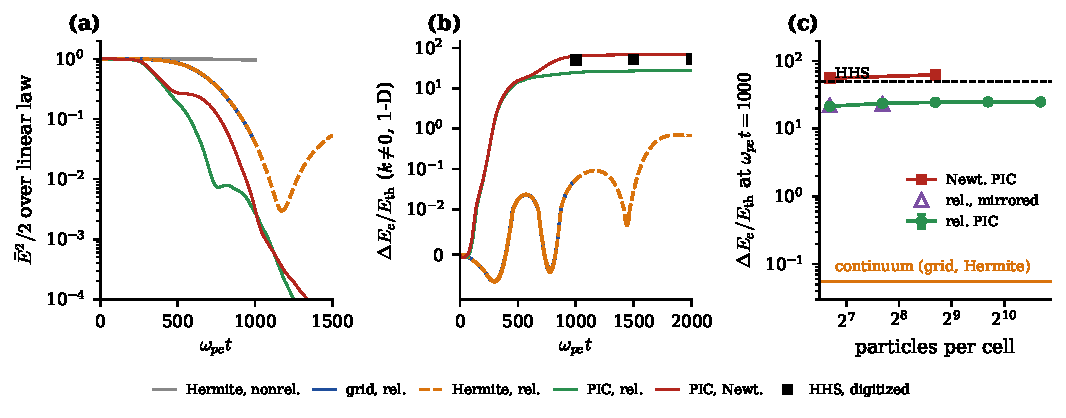
\includegraphics[width=\textwidth]{figures/fig_hhs.pdf}
\caption{Resonant drive $\vq=0.03$ (figure of the paper). (a) Mean-field energy over the exact linear law (trailing $200\,\wpe^{-1}$ mean) for the nonrelativistic Hermite model, the relativistic grid, the relativistic Hermite model and the relativistic and Newtonian PIC. (b) HHS measure of the $k\ne0$ electron energy change over $\Eth$ (symmetric logarithmic scale); squares: HHS Fig.~2 re-digitized. The continuum curves coincide to $\wpe t=1000$ and remain below $\sim1\,\Eth$ to $2000$. (c) Heating at $\wpe t=1000$ against particles per cell, with the relativistic plateau, the Newtonian PIC, mirrored loading, the HHS value and the continuum value.}\label{fig:c10-hhs}
\end{figure}

\chapter{Analysis and discussion}\label{ch:discussion}

The preceding chapters are written in the order in which the work was done, which is also the order in which its premises were found wanting. This chapter reverses the perspective. It sets out what the records establish and what they do not, gives a physical picture that is consistent with all of them without claiming more than they support, discusses what can and cannot be said about the cosmological bounds, draws the methodological lessons we would apply again, and ends with the open questions and a concrete plan for answering them.

\section{What is established and what is not}

Four statements are, in our judgement, established, each by at least two independent calculations and each with its checks declared before the runs.

The first is that in the nonrelativistic Hermite model the work done by a resonant uniform drive follows the exact linear law within the certified windows of Table~\ref{tab:c9-win}, to $0.7\,\%$ at $\vq=0.07$ and a corresponding or smaller deficit at $0.03$ and $0.05$, with no resolved frequency shift. The residual is a seed back-reaction that scales as the square of the imposed fluctuation level and not as a property of the drive. The windows are a property of the instrument, not of the plasma. This statement is about a model whose coherent speed reaches $0.47$--$0.87c$ at the window end, and it holds for the model only.

The second is that relativity alone detunes the uniform resonance, and does so on a time scale that agrees with the loss of the resonance in HHS. The exact homogeneous relativistic kinetic equation, the relativistic grid with deterministic seeds and the relativistic Hermite model with deterministic seeds give a $10\,\%$ departure of the work from the linear law at $\wpe t=392$, $392$ and $392.5$ for $\vq=0.03$, and the grid and the exact equation give $1309.5$ and $1429$ at $\vq=10^{-3}$; the nonrelativistic grid with the same noise gives $770$--$870$ at $0.03$ and no departure at $10^{-3}$ to $3000$. The coherent mass increase of Eq.~\eqref{eq:duffing} accounts for the strong-drive number at the level of an estimate, and the thermal shift of the plasma frequency accounts for the weak-drive one, as the slow-flow model of Section~\ref{sec:relativistic} shows by giving no collapse for the weak drive without it. In the PIC the departure is earlier ($273$--$311$) because it is noise-assisted, and the Newtonian PIC shows that noise alone suffices for a $10\,\%$ departure.

The third is that an independent relativistic PIC converges, in particle number from 103 to 1648 per cell, in cell size from $0.04$ to $0.01\,c/\wpe$, in time step and in shape order, to a heating of $\simeq25\,\Eth$ at $\wpe t=1000$ in the HHS measure, and that a Newtonian pusher with the same code gives $2.5$ times more. The re-digitized HHS curve is $50.1\,\Eth$, so the plateau is half of it.

The fourth is that deterministic continuum models, with a ledger closing to $10^{-8}$ in the Hermite case, give $0.056\,\Eth$ at $\wpe t=1000$ whatever the discretization, and remain below $0.7\,\Eth$ to $2000$, a factor $445$ below the PIC plateau; and that continuum models given PIC-like noise lose positivity before the heating can develop.

Five things are not established. We do not know why our PIC plateau is a half of the HHS value. We do not know what seeds the PIC heating, beyond the exclusion of long-wavelength current noise by the mirrored loading and of a $1/N_{\rm ppc}$ noise law by the plateau. We do not know whether a positive, converged continuum initial condition with fluctuation spectrum equal to the PIC's would produce the same heating; our attempts failed on positivity, which is a property of the discretization and not a physical finding. We do not know whether the heating survives in two or three dimensions, where the instabilities that HHS invoke are not confined to the axis of the drive. And we do not know the consequence for the cosmological bounds, since no calculation here had cosmological parameters. The deterministic nonrelativistic nonlinear cascade, which the nonrelativistic windows end just before, was not resolved.

\section{A physical picture}

The picture that fits the records has two parts, which should be separated because they have different status.

The first part is established. A uniform resonant drive accelerates the electrons coherently, with speed growing as $v_q\,t/2$. Because the mass increases with the speed, the plasma frequency falls and the drive, held at the cold frequency, moves out of phase with the response. The mean-field response switches off when the accumulated phase mismatch of Eq.~\eqref{eq:slowflow}, $v_q^2t^3/64$ for a cold plasma, reaches order unity, that is at a time that scales as $v_q^{-2/3}$ and is of the order of $400$ plasma periods for $\vq=0.03$. This is a statement about a single coherent degree of freedom, it requires no fluctuations and no instability, and it explains why the physical mean field collapses at the time at which HHS see it. It is in this sense that detuning switches off the coherent pump. It is not an attractive mechanism for cosmological conclusions because it leaves the electron energy where it is: the work done by the drive up to the collapse sits in the coherent quiver and remains there, in a state in which each electron carries a large coherent momentum. Relativistic detuning alone would therefore limit the \emph{coherent} transfer without thermalizing it.

The second part is a hypothesis. The coherent state is not stable against the fluctuations present in any real plasma. Once the quiver is large the plasma is subject to the oscillating-two-stream and modulational instabilities that HHS describe, whose growth requires seeds. The PIC has a broadband seed from the finite number of particles, the continuum codes have none beyond the smooth one we gave them, and what separates the two is a factor $445$ in the heating. If the heating is seeded by fluctuations near the cell scale, as the mirrored loading and the plateau suggest and cannot prove, then the energy from the coherent quiver reaches the thermal distribution through a cascade of the kind HHS propose, in which noise at high $k$ grows fastest and the nonlinear state is dominated by it. The question that this raises is not whether such a cascade exists, since both PICs show it, but how its outcome depends on the seed spectrum. In a real early-universe plasma the seed spectrum is that of thermal fluctuations of the actual plasma, with a physical particle number per Debye volume enormously larger than a PIC can afford, so the fluctuation level at any $k$ is much smaller than a PIC's. The PIC plateau being independent of particle number over a factor of 16 would then be reassuring if the plateau had a physical cause; and worrying if it only means that a floor set by the cell is being hit, which the statement ``near the cell scale'' would imply. It is the central ambiguity of the whole study.

\section{Implications for the cosmological bounds}

A cautious reading is required. HHS conclude that the bounds from resonant conversion fail because the transfer saturates at roughly the thermal energy. What we found does not contradict the possibility that the coherent transfer is cut off, and the cut-off by relativistic detuning is robust within the one-dimensional, uniform, collisionless model. What we found does not demonstrate that the energy deposited is limited to the thermal energy either, since three further statements need to be true and none is established here.

The first is that the mean-field collapse limits the \emph{total} energy transferred, which assumes that no further energy is delivered once the coherent response is gone. In the deterministic relativistic models the energy delivered up to the collapse stays in the coherent quiver, and the model is silent about what happens to it afterwards. In the PIC the heating reaches $25\,\Eth$ and stays there to $2000$ ($28\pm3.7$), so the energy sits at the level of tens of thermal energies, and the question of the late deposition rate is not answered by a run of $2000$ plasma periods when the resonance lasts, in HHS' estimate, $10^{10}$.

The second is that the inhomogeneity needed for conversion in the early universe (the Landau--Zener passage) behaves like a uniform drive in a box. Our inhomogeneous calculations are linear and relativistic in $k$, and say that the transverse transmitted fraction follows a Landau--Zener exponent corrected by a factor $1-4.5s^2$ with $s=\eta n_c/\bar k^2$ (the notation of Section~\ref{sec:c9-r3}); in the cosmological regime the dark-photon momentum is tiny and the parameter $s$ is not necessarily small, so the standard exponent may be out of its domain. We did not test this regime.

The third is the collision frequency. Equation~\eqref{eq:c9-pss} gives a steady absorbed power inversely proportional to $\nu_{\rm eff}$ at resonance, and the numbers in HHS' Eqs.~(6) and~(7) set $\nu_{ei}\propto T_e^{-3/2}$ and an energy-exchange time $\tau_{ei}\propto T_e^{3/2}$ that grow strongly with temperature. An electron temperature $10^{2}$ times the initial one reduces $\nu_{ei}$ by $10^{3}$, and in the steady state the resonant absorption grows with the inverse of $\nu_{ei}$, which means the heating would raise the deposited power; but the amplitude transient has a time $4/\nu_{ei}$ that grows by the same factor, so the steady state would never be reached. The competition between the two is a matter of the actual Spitzer law and the actual cosmic expansion time, which our constant-$\nu$ runs cannot decide. The relativistic correction to the collision operator is also not available.

The conditional statement we are prepared to make is therefore the following. In the model of one dimension, uniform prescribed drive, constant collision rate and no cosmology, the resonant coherent transfer is cut off by relativistic mass increase at a time much shorter than the resonance time of any cosmological crossing, and the energy that reaches the thermal distribution in a relativistic PIC is of the order of tens of initial thermal energies at $\wpe t=2000$. Whether this implies that the bounds are weakened by the factors that HHS state depends on the late-time deposition, the actual collision law and the dimensionality, and the calculations here do not decide it. We have not computed, and do not give, any revised bound.

\section{Methodological lessons}

Several practices proved their value and are worth stating plainly, since they shaped what could be concluded.

The first is the certified window. A Hermite run that ends in a NaN is easy to detect; a run that stays finite and produces a plausible curve for 200 time units after it should have been abandoned is not. Defining the window in advance as the smallest of four times (refinement pairs agreeing to $10\,\%$, positivity, reaching the time, ledger closure) removed the temptation to plot until the curve looked wrong. The windows of Chapter~\ref{ch:nonrel} are short of $1000$ for the stronger drives, and the relativistic Hermite horizon of F1 fell short of its declared $2000$; both facts are in the tables, not in the discussion of the figures.

The second is declaring the gates before running and not amending them. The repository contains many failures that would have been invisible otherwise: the realized phase variance of the first coherence study, the ledger gates D and D2 of the grid, the spectrum check c of the relativistic Hermite model, which was wrong because a truncated Hermite matrix has an undamped discrete spectrum, the zero-collision rerun that differed from an old record by $6\times10^{-6}$ because the restart chunk was 200 and not 240, and the PIC convergence gates G4 and G5. In each case the failure was reported, a follow-up was declared in a new commit before it was run, and the claim was changed to what the follow-up supported. The cost is a long list of failed checks. The benefit is that a reader can see which numbers were tested against what.

The third is the independent reference. Every pair of agreeing calculations in the note (the Hermite and the grid at $392$ and $392.5$; the Landau roots from the relativistic grid against the kinetic roots; the two collision operators against one another and against the exact driven oscillator with drag; the cold-fluid and kinetic transverse conversion) is a protection against a common error, and the one place at which no independent reference exists, the heating, is where we are least sure what we know. The mistake over the HHS digitization was of the same kind from the other side: a single reading of a single curve was relied on as if it were an independent reference, and it was not.

The fourth is that agreement of a resolved calculation with a theory is silent about what happens beyond the window. The bound of Chapter~\ref{ch:nonrel} says that no saturation appears before the cascade starts, and it says nothing of the cascade. The corresponding sentences are written into each section and into the abstract of the paper, and we would keep them even if they weaken the statements.

\section{Open questions and a research plan}

The questions follow from the five items above. The plan below orders them by what each would settle and by cost. None of it has been run.

The first and cheapest step is a scan of the cell-scale noise. The PIC at 412 particles per cell and $\Delta x=0.02$ is the missing combined point, and it would directly test whether the combination of the two refinements adds to the $15\,\%$ or counts the same effect twice, as we argue. A broader scan would add a controlled injection of noise at a chosen $k$ in a PIC with a quiet start: a quiet start (mirrored velocities and regularly spaced positions) with a seed of known spectrum, amplitude and cutoff, so that one can read off the heating as a function of the seed at $k\lambda_{De}$ from $0.1$ to the cell Nyquist. If the plateau persists at a seed amplitude that is physical, the heating is robust; if it scales with the amplitude at the cell scale it is a numerical floor. The scan needs a PIC only, and the cost per run is that of the ladder above (hours on a few cores).

The second step is the shape function. The HHS code uses fifth-order splines in deposition and force interpolation; our quintic test showed a $4\,\%$ change at 412 particles per cell, but at one particle number and with a different pusher, and a combined test of fifth order with 1648 particles per cell and a smaller cell would remove the main code-level candidate for the factor of two. This is a parameter of the code we already have.

The third step is the relativistic Hermite model with a stabilised closure. The model is certified to about $1530$ and the shot-noise runs fail at once for the PIC particle number. A path to the noisy regime requires a method that preserves positivity or that damps the top of the ladder without changing the lowest moments; the options tested in the nonrelativistic case (Dai, symmetric weight, square-root form) fail their nonlinear gates at $\vq=0.1$ and have not been tried in the relativistic code. We regard the matter as unsettled, with the Hermite route not closed. A closure scaling with the local field, as in the nonrelativistic code, together with a hypercollision of the type that passed the $1\mathrm{D}2\mathrm{V}$ test, is the nearest candidate.

The fourth step is two dimensions. The instabilities invoked by HHS for the transfer of energy have a direction, the drift, and the argument for one dimension is that the fastest modes are aligned with it. A two-dimensional PIC with a mixed field would test whether the heating is the same, larger or smaller, and whether the $k=0$ resonance is detuned in the same way. The relativistic grid and Hermite models have the cost structure to do one dimension in $x$ and two in $u$ only for small $N_x$.

The fifth step is cosmological deposition. The collision law needs the Spitzer frequency $\nu_{ei}(T_e)\propto T_e^{-3/2}$ in the absorption equation, a relativistic correction, an expansion rate and cooling. With these the question becomes a closed, zero-dimensional or one-dimensional model whose deposited energy can be computed as a function of $\vq$ and $\omega_{pe}/H$ and compared with the bound; it uses Eq.~\eqref{eq:c9-drude} with a temperature-dependent $\nu$ and the heating of the PIC as an energy input, and it is the calculation that turns the present study into a statement about cosmology. It needs the answer to the heating questions first, because the input is the heating.

The remaining items, none large, are: a record of the thermal relativistic shift of the plasma frequency to confirm the weak-drive collapse time; a direct comparison of the Vay and Boris pushers in the resonant case; the Gaussian line and the combined reservoir and coherence run of Chapter~\ref{ch:nonrel}; and the missing seed levels in the back-reaction study.

\appendix
\chapter{Reproducibility}\label{app:repro}

This appendix says where the code and the records are, which versions of which repositories produced them, how each study is rerun, and where the unmerged parent pull requests stand. Paths are relative to the repository root. No record contains a machine path, and none of the commands needs one. The statements about pins are those of the paper's data-availability section and of \texttt{docs/status.md} at commit \texttt{3d9eb3a}, the head of \texttt{main} when this chapter was written.

\section{Repositories and pins}

The work is spread over four repositories, and the dependence between them is part of what a reader needs to reproduce a number.

\emph{Dark-SPECTRAX} (\texttt{uwplasma/Dark-SPECTRAX}) holds the dark-photon extension, all the study scripts and records, \texttt{docs/results.md} (generated from the records by \texttt{docs/make\_results.py}), \texttt{docs/status.md}, and the paper in \texttt{paper/} whose figures, numbers and tables are generated by \texttt{paper/make\_figures.py}. No release or tag has been made. The records and scripts of the paper are those of commit \texttt{eb36319}; the relativistic grid records carry \texttt{a5aab9f}, the relativistic Hermite records \texttt{0873d10} and the nonrelativistic studies \texttt{a3ef7a6}.

\emph{SPECTRAX} (\texttt{uwplasma/SPECTRAX}) is the parent Hermite--Fourier solver. Dark-SPECTRAX does not run against its \texttt{main}: it is pinned to an integration branch that merges the open pull requests of the author that the studies need. Three pins appear in the records. The reservoir and coherence study used \texttt{3de6b2b}, the strong-drive study \texttt{4090fbe}, and the collision studies \texttt{35231ab}, all on \texttt{integration/dark-baseline}. The relativistic Hermite studies used \texttt{6a6606b} on \texttt{integration/dark-baseline-2}, which is SPECTRAX main \texttt{32f7d81} with the open pull requests merged, then PR 88 (the relativistic option, \texttt{inv\_c2}), then a commit that makes the pump-frame initial state \texttt{F0} work in the relativistic branch (branch \texttt{feature/relativistic-pump-frame}, fast-forward merged into the integration branch; it has no pull request of its own because it needs \texttt{F0}, which only the integration branch has). The repository records state that the same inputs reproduce bitwise on both integration branches for the checks done. None of these branches is a release.

\emph{JAX-in-Cell} (pin \texttt{2d693cb}) and \emph{Dark-JAX-in-Cell} (pin \texttt{d547579}) hold the PIC. The pusher is a relativistic Boris/Vay-family one in JAX-in-Cell with \texttt{Solver(relativistic=True)} and shape order 2 or 5; Dark-JAX-in-Cell adds the dark-photon drive and the paper-replay example. The grid solver of Chapter~\ref{ch:rel} uses NumPy and SciPy only.

The environment for the production runs was a CPU virtual environment with JAX 0.6.2 and Python 3.10 on the shared compute host for the PIC and the grid, and the laptop (Python 3.13) for the first relativistic Hermite runs. The GPU resolution study used JAX 0.11.2 with CUDA 12 in double precision. The GPU/CPU comparison for one short case differs by $9.7\times10^{-9}$.

\section{Rerunning each study}

Every study follows the same pattern: a script declares its gates and its run list and is committed before any run (\texttt{*\_gates.py}); a driver or batch script runs the cases in chunks that can be resumed from a checkpoint; an analysis script produces a summary record in JSON; and \texttt{docs/make\_results.py} turns the summaries into \texttt{docs/results.md}. The heavy runs take the lock \texttt{/tmp/spectrax-heavy.lock} (a directory created with \texttt{mkdir}) so that at most one runs at a time on a shared machine. The commands below are the entry points, not a transcript; the arguments are in the scripts' docstrings.

The nonrelativistic strong-drive and truncation studies are \texttt{studies/nxconv\_*.py} (Nx convergence against the spectral grid), \texttt{studies/highk\_*.py} (the truncation instability, the closure, the Floquet and eigenvalue checks), \texttt{studies/nxconv/batch11.sh} (the wide-box grid reference), \texttt{studies/gpures\_gates.py} with \texttt{gpures\_batch.sh} (the GPU resolution extension), and \texttt{studies/rclosure\_gates.py} with \texttt{rclosure\_analysis.py} (the closure-strength study). The three rejected alternative bases are in \texttt{studies/dai}, \texttt{studies/sw} and \texttt{studies/antisym}.

The finite reservoir and coherence study is \texttt{studies/r1\_common.py} (gates and linear theory), \texttt{r1\_reservoir.py} and \texttt{r1\_coherence.py}; the strong-drive windows and the seed back-reaction are \texttt{studies/r1nl\_gates.py}, \texttt{r1nl\_run.py} run through \texttt{r1nl\_batch.sh} (200-unit chunks), \texttt{r1nl\_analysis.py} and the follow-up \texttt{r1nl\_followup.py}. Collisions are \texttt{studies/r2\_gates.py}, \texttt{r2\_batch.py WORKERS [filter]} (a worker pool, each case chunked and resumable), \texttt{r2\_analysis.py} and \texttt{r2\_followup.py}, and the LBO-G comparison \texttt{studies/h08\_lbog.py}. Inhomogeneous conversion is \texttt{studies/r3\_gates.py}, \texttt{r3\_ref.py} (the independent cold reference), \texttt{r3\_kin.py} with \texttt{r3\_kin\_batch.sh}, \texttt{r3\_analysis.py}, and the follow-ups declared in \texttt{r3\_followup\_gates.py} with \texttt{r3\_followup\_batch.sh}.

The relativistic grid is \texttt{studies/relgrid.py} with \texttt{relgrid\_gates.py}, \texttt{relgrid\_ref.py} (the exact homogeneous ODE, the cold fluid and the J\"uttner dispersion), \texttt{relgrid\_driver.sh} (gate C2 and the queued parts), \texttt{relgrid\_batch.sh} and \texttt{relgrid\_batch2.sh}, \texttt{relgrid\_office.sh} (the runner used on the shared host) and \texttt{relgrid\_analysis.py}. The relativistic Hermite model is \texttt{studies/relherm/} (gates and the 1D2V checks), \texttt{studies/relhhs\_gates.py}, \texttt{relhhs\_run.py} through \texttt{relhhs\_batch.sh NX NN C} with \texttt{SPECTRAX\_SRC} pointing to a checkout at \texttt{6a6606b}, and \texttt{relhhs\_analysis.py}; its design note is \texttt{docs/design/relativistic-hermite.md}. The $k$-range study is \texttt{studies/hkr\_gates.py}, \texttt{hkr\_grid.py}, \texttt{hkr\_hermite.sh}, \texttt{hkr\_par.sh} and \texttt{hkr\_analysis.py}.

The PIC studies are \texttt{studies/relpic/gates.py}, \texttt{relpic\_run.py}, \texttt{batch.sh} and \texttt{batch\_parallel.sh} (the first twelve runs and the Newtonian controls), then \texttt{conv\_gates.py}, \texttt{conv\_followup\_gates.py}, \texttt{batch\_conv.sh TAG CORES LOGDIR} (one tag of the ladder per call, with the environment variables \texttt{DJIC}, \texttt{JIC} and \texttt{PY} naming the Dark-JAX-in-Cell checkout, the JAX-in-Cell checkout and the interpreter) and \texttt{conv\_analysis.py}. The digitization of the HHS figure is in \texttt{studies/relpic/digitization/}. The single-particle pusher checks are in \texttt{studies/relpic/single\_particle.json}. The paper figures and numbers regenerate with \texttt{python paper/make\_figures.py} from the repository root.

The tests (\texttt{tests/}) run with \texttt{pytest -n 2}, 91 tests locally at the last relativistic commit, and the continuous-integration workflow runs them on two Python versions. Heavy PIC and grid runs are not part of the tests.

\section{Record index}

Table~\ref{tab:a-index} maps the chapters of this part to their records.

\begin{table}[t]
\centering
\caption{Records behind the chapters (paths relative to the repository root).}\label{tab:a-index}
\small
\begin{tabular}{@{}p{3.6cm}p{9.6cm}@{}}\toprule
Topic & Records\\\midrule
Windows, truncation instability & \texttt{studies/nxconv/summary.json}, \texttt{studies/highk/eig.json}, \texttt{studies/gpures/summary.json}, \texttt{studies/rclosure/stagef.json}, \texttt{studies/r1nl/stage1\_summary.json}\\
Seed back-reaction, reservoir, coherence & \texttt{studies/r1nl/stage2\_summary.json}, \texttt{followup\_summary.json}, \texttt{studies/r1/reservoir\_summary.json}, \texttt{coherence2\_summary.json}\\
Collisions, LBO-EM and LBO-G & \texttt{studies/r2/summary.json}, \texttt{studies/h08/summary.json}, \texttt{studies/h08\_lbog/}\\
Conversion at a ramp & \texttt{studies/r3/} (reference and kinetic records, follow-ups F and G)\\
Relativistic grid & \texttt{studies/relgrid/summary.json}, \texttt{homog.json}, \texttt{gates\_*.json}, \texttt{runs/}\\
Relativistic Hermite & \texttt{studies/relherm/gates\_*.json}, \texttt{studies/relhhs/summary.json}, \texttt{gates\_*.json}, \texttt{runs/}\\
$k$-range grid & \texttt{studies/hkr/summary\_grid.json}, \texttt{studies/hkr/validation*.json}\\
PIC and HHS digitization & \texttt{studies/relpic/conv\_summary.json}, \texttt{records/}, \texttt{digitization/hhs\_fig2.json}, \texttt{single\_particle.json}\\
Status and failed checks & \texttt{docs/status.md}, \texttt{docs/results.md}, Table~II of the paper\\\bottomrule
\end{tabular}
\end{table}

\section{Parent pull requests}

The pull requests of SPECTRAX that the studies depend on were all opened by the author and none, at the time of writing, is merged except as noted. The list is from \texttt{docs/upstream-review.md}, updated at the resync of 2026-10-25, when main was at \texttt{32f7d81}. Merged into main by the owner since the first review: 46, 48, 12, 13, 50 (at \texttt{b668d87}) and 86 (Python 3.10 support, which supersedes the \texttt{requires-python >=3.11} set by 48). Open and carried on the integration branch: 9, 55, 44, 18, 51, 21, 34, 62, 63, 64, 65 (output, state, configuration and input features), the adaptive-stepping base and 56 to 61 (remapping and pump frame), 66 (field-scaled closure, used by every strong-drive study), 72 (its magnetic option), 68 to 70, 71 (the Dougherty collision operator, LBO-EM), 73 (LBO-G, $\beta=0$) and 88 (relativistic Hermite). PR 21 still conflicts with PR 18, which both implement a midpoint integrator. The PR 88 code has no syntax that requires Python 3.11. A full test run of the merged integration branch gave 247 passed and one expected failure under Python 3.12; under Python 3.10 with JAX 0.6.2 one test segfaults inside XLA compilation, and it does so on a clean \texttt{main} too. The records of the studies stay valid across the repins because the repins only add features that are off by default; the check of bitwise equality for a seeded pump-frame run before and after the repin of 2026-10-16 is in \texttt{docs/status.md}. Nothing was merged into SPECTRAX main by the studies, and no pull request was closed.

\bibliographystyle{unsrtnat}
\bibliography{refs}
\addcontentsline{toc}{chapter}{Bibliography}
\end{document}
